\documentclass[titlepage,letterpaper,final]{scrartcl}

\usepackage{scrindex}           % multiple index support using the "index" package
\usepackage{index}

% This file contains macros included in manual.tex and forcing.tex, in the preamble.
% This way we have all the URLs and such in one place.

%% THE FOLLOWING SHOULD CHANGE FOR A STABLE RELEASE:
\newcommand{\PISMREV}{revision \texttt{@Pism_REVISION_TAG@}}
\newcommand{\PETSCREL}{3.2}
\newcommand{\PISMDOWNLOADMSG}{Get development branch source code:
  \quad \texttt{git clone -b dev git@github.com:pism/pism.git pism-dev} \quad}
\newcommand{\PISMBROWSERURL}{http://www.pism-docs.org/wiki/doku.php?id=browser}
\newcommand{\PISMEMAIL}{\href{mailto:help@pism-docs.org}{\texttt{help@pism-docs.org}}}

\newcommand{\normalspacing}{\renewcommand{\baselinestretch}{1.1}\tiny\normalsize}
\newcommand{\tablespacing}{\renewcommand{\baselinestretch}{1.0}\tiny\normalsize}
\normalspacing

\usepackage[usenames]{xcolor}

\usepackage{bm,url,xspace,verbatim}
\usepackage{amssymb,amsmath}
\usepackage[pdftex]{graphicx}

\usepackage{booktabs}           % better rules in tables
\usepackage[nohyphen]{underscore}

\newcommand{\ddt}[1]{\ensuremath{\frac{\partial #1}{\partial t}}}
\newcommand{\ddx}[1]{\ensuremath{\frac{\partial #1}{\partial x}}}
\newcommand{\ddy}[1]{\ensuremath{\frac{\partial #1}{\partial y}}}
\renewcommand{\t}[1]{\texttt{#1}}
\newcommand{\Matlab}{\textsc{Matlab}\xspace}
\newcommand{\bq}{\mathbf{q}}
\newcommand{\bU}{\mathbf{U}}
\newcommand{\eps}{\epsilon}
\newcommand{\grad}{\nabla}
\newcommand{\Div}{\nabla\cdot}

%% macros having to do with documentation for options; note these appear in the index

\newindex{default}{idx}{ind}{General Index}
\newindex{options}{odx}{ond}{PISM Command-line options}

\def\optsection#1{%
  \def\optindex##1{\index[options]{#1!##1}}
  \def\optseealso##1{\index[options]{#1|see{##1}}}
}

\optsection{FIXME}

% Use this to index option definitions:
\newcommand{\intextoption}[1]{\texttt{-#1}\optindex{\texttt{-#1}}}

\newcommand{\txtopt}[2]{\texttt{-#1} #2\optindex{\texttt{-#1} #2}}

\newcommand{\listopt}[1]{\txtopt{#1}{\emph{comma-separated list}}}
\newcommand{\fileopt}[1]{\txtopt{#1}{\emph{filename}}}
\newcommand{\timeopt}[1]{\txtopt{#1}{\emph{range or list}}}

\def\variable#1{\texttt{#1}\index{NetCDF variables!\texttt{#1}}}
\def\config#1{\texttt{#1}\index{Configuration flags and parameters!\texttt{#1}}}
\def\class#1{\texttt{#1}\index{C++ classes!\texttt{#1}}}


%\addtolength\topmargin{-.1in}
\addtolength\textheight{0.75in}
\addtolength{\oddsidemargin}{-.4in}
\addtolength{\evensidemargin}{-.4in}
\addtolength{\textwidth}{0.9in}

%% uncomment to see locations of index entries
% \proofmodetrue

% this lets us avoid the scrartcl/hyperref conflict...
\let\ifvtex\relax

% hyperref should be the last package we load
\usepackage[pdftex,
colorlinks=true,
plainpages=false, % only if colorlinks=true
linkcolor=blue,   % only if colorlinks=true
citecolor=blue,   % only if colorlinks=true
urlcolor=blue     % only if colorlinks=true
]{hyperref}

\pdfinfo{
/Title (PISM User's Manual)
/Author (the PISM authors)
/Subject (Using PISM, a Parallel Ice-Sheet Model)
/Keywords (PISM ice sheet modeling)
}

\begin{document}
\graphicspath{{figs/}}

\begin{titlepage}

  \begin{center}
    {\huge\usekomafont{title} \emph{PISM}, a Parallel Ice Sheet Model:\\\medskip User's Manual}
    \vspace{0.5cm}

    {\Large The PISM Authors}
    \vspace{1cm}

    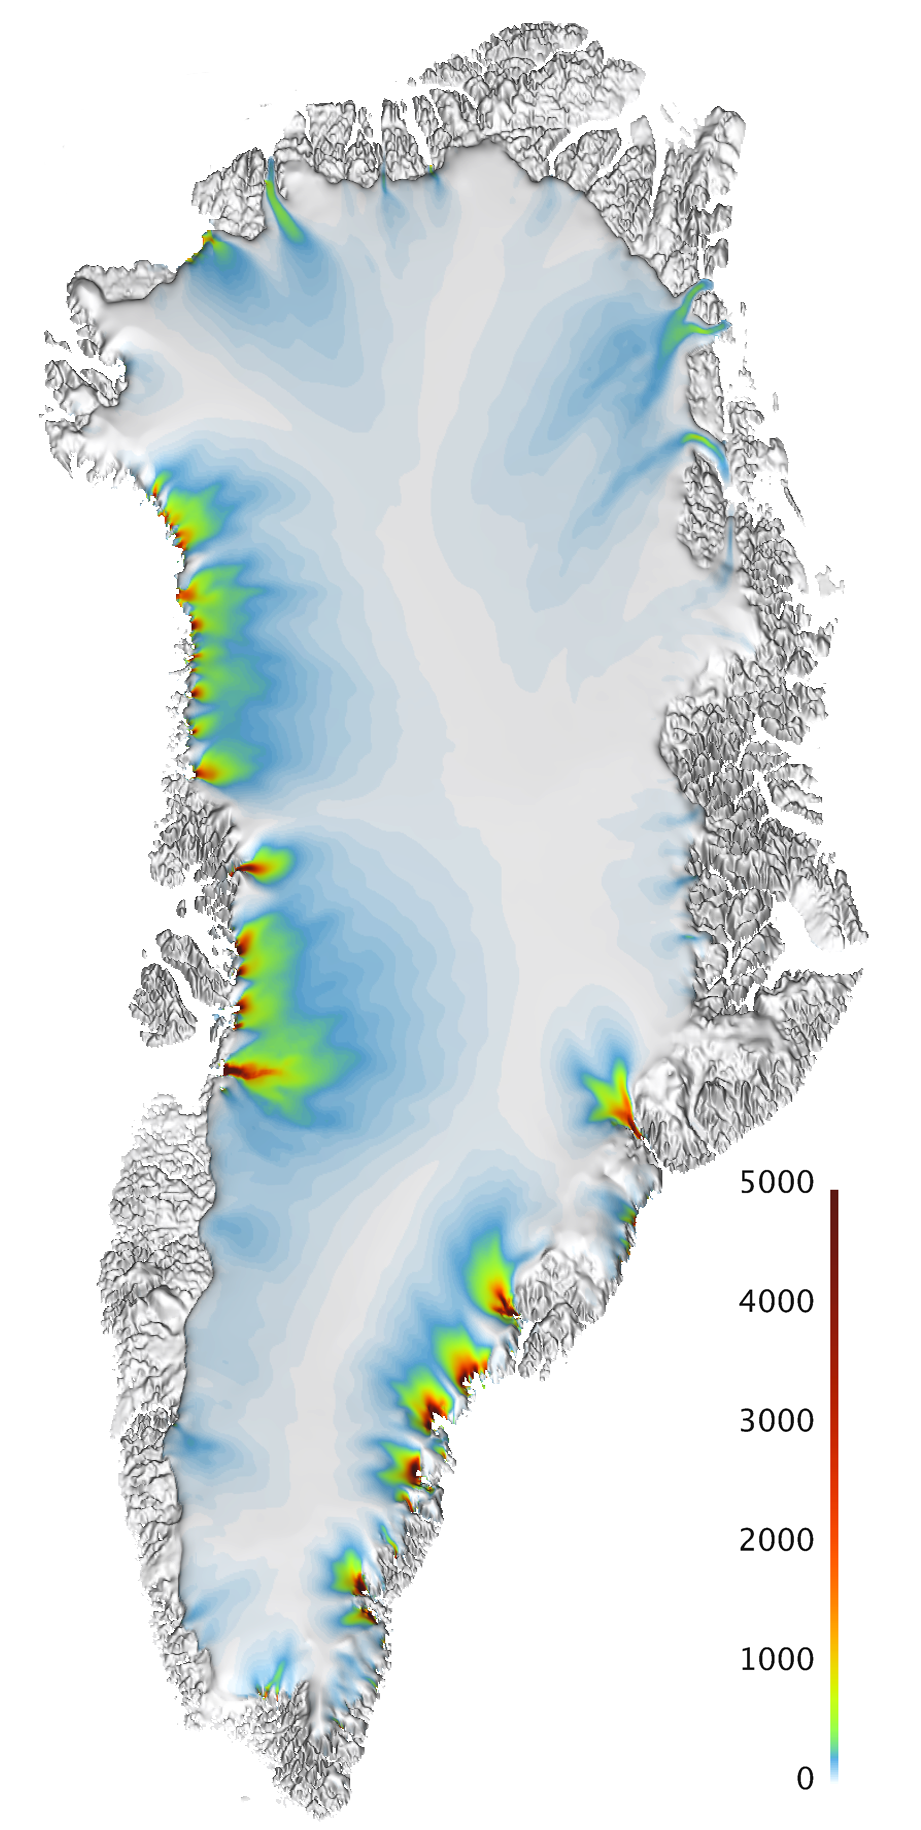
\includegraphics[width=3.3in,keepaspectratio=true]{grn-1km-csurf}
    \vfill

    \small Support by email: \PISMEMAIL.
    \medskip

    Manual date \today. Based on PISM \PISMREV.
    \medskip

    \PISMDOWNLOADMSG
  \end{center}
\end{titlepage}

\newpage
\phantom{bob}

\centerline{\textsc{Authorship}}
\bigskip

\normalspacing
PISM is a joint project between developers in the ice sheet modeling group at the University of Alaska (UAF) and at the Potsdam Institute for Climate Impact Research (PIK).  The number of source code authors, documentation authors, and script contributors is large. Perhaps the best description is this alphabetical list.
\bigskip
\normalspacing

\renewcommand{\arraystretch}{1.3}
\begin{tabular}{ll}
\textbf{Torsten Albrecht} & ice shelf physics and numerics \\
\textbf{\underline{Andy Aschwanden}} & \begin{minipage}[t]{4in} scripts, visualization, thermodynamics, SeaRISE-Greenland, Storglaci\"aren  \end{minipage}  \\
\textbf{Jed Brown} & source code original author, SSA numerics, PETSc underpinnings \\
\textbf{\underline{Ed Bueler}} & \begin{minipage}[t]{4in} principal investigator, verification, earth deformation, SIA, thermodynamics, documentation  \end{minipage} \\
\textbf{Dani DellaGiustina} & regional tools and modeling \\
\textbf{Marijke Habermann} & inversion\\
\textbf{Marianne Haselhoff} & ice streams: physics and numerics\\
\textbf{Regine Hock} & surface mass and energy balance \\
\textbf{\underline{Constantine Khroulev}} & \begin{minipage}[t]{4in} source code primary author, input/output, software design, climate couplers, parallelization, testing, user support, most documentation, most bug fixes, regional tools \end{minipage} \\
\textbf{Craig Lingle}\index{People!Lingle, Craig} & original modeling choices, earth deformation, modeled-it-before-you-did \\
\textbf{Maria Martin} & SeaRISE-Antarctica, Antarctica processes \\
\textbf{Mattias Mengel} & marine ice sheet processes \\
\textbf{David Maxwell} & inversion, SSA finite elements, python bindings \\
\textbf{Ward van Pelt} & hydrology analysis and design \\
\textbf{Nathan Shemonski} & EISMINT-Greenland example \\
\textbf{Ricarda Winkelmann} & Antarctica processes, coupling, and modeling  \\
\textbf{Florian Ziemen} & bug fixes, sliding \\
\end{tabular}

\bigskip\bigskip
Users will reach the \underline{underlined} UAF-based developers listed above by using the email address

\centerline{ \PISMEMAIL.  }

\bigskip\bigskip
\noindent \textsc{Front page}:  Magnitude of horizontal surface velocity from PISM run on a horizontal grid resolution of 1\,km.  Visualization by IDV.

\vfill

\newpage
\vspace{0.2in}
\begin{quote}
\textsl{Copyright (C) 2004--2012 The PISM Authors}
\medskip

\noindent \textsl{This file is part of PISM.  PISM is free software; you can redistribute it and/or modify it under the terms of the GNU General Public License as published by the Free Software Foundation; either version 2 of the License, or (at your option) any later version.  PISM is distributed in the hope that it will be useful, but WITHOUT ANY WARRANTY; without even the implied warranty of MERCHANTABILITY or FITNESS FOR A PARTICULAR PURPOSE.  See the GNU General Public License for more details.  You should have received a copy of the GNU General Public License\index{GPL (\emph{GNU Public License})} along with PISM; see \emph{\texttt{COPYING}}.  If not, write to the Free Software Foundation, Inc., 51 Franklin St, Fifth Floor, Boston, MA  02110-1301 USA}
\end{quote}
\vspace{0.5in}

\centerline{\textsc{Acknowledgements}}
\bigskip

\small
The NASA Modeling, Analysis, and Prediction program\index{Organizations!NASA!Modeling, Analysis, and Prediction Program} (grant \# NNX09AJ38G) supports the development of PISM from 2009 to 2013.  Development from 2002 to 2008 was supported by the NASA Cryospheric Sciences Program\index{Organizations!NASA!Cryospheric Sciences Program}.  The Snow, Ice, and Permafrost (SIP) group\index{Organizations!Geophysical Institute!Snow, Ice, and Permafrost group} at the Geophysical Institute is the home for the University of Alaska PISM developers; find us in Elvey 410D.  The Arctic Region Supercomputing Center\index{Organizations!Arctic Region Supercomputing Center (ARSC)} has provided significant computational resources and technical help in the development of PISM.

Thanks for comments/questions from many PISM users around the world, including

\begin{quote}
Tolly Adalgeirsdottir, Antje Fitzner, Nick Golledge, Tore Hattermann, Marianne Madsen, Malou Maris, Art Mahoney, Kent Overstreet, Sebastian Simonsen, Anne Solgaard, Ben Sperisen, Martin Truffer, Shuting Yang, Ryan Woodard
\end{quote}

\noindent for helpful comments and questions on PISM and this \emph{Manual}.  Dave Covey, Don Bahls, and Greg Newby have supported our hardware, software, and computations.  Bob Bindshadler, Sophie Nowicki, Jesse Johnson, and others in the SeaRISE group have motivated and assisted PISM development in many ways.  

\normalsize



\newpage
\setcounter{tocdepth}{3}
\small
\tableofcontents
\normalsize

\newpage


\section{Introduction}\label{sec:intro}

Welcome!  All information about PISM is online at the home page
\begin{center}
  \url{http://www.pism-docs.org}
\end{center}
Please see the extensive lists of PISM applications and user projects at the home page.

This User's Manual gives examples of how to run PISM using publicly-available data for: the whole Greenland ice sheet, the Jakobshavn outlet glacier in Greenland, the Ross ice shelf in Antarctica, and the St\"orglaciaren mountain glacier in Sweden.  It documents all the PISM options.  It summarizes the continuum models used by PISM, and it illustrates how PISM's numerical approximations are verified.

See the PISM Installation Manual\footnote{PDF for latest stable release at \url{http://www.pism-docs.org/wiki/lib/exe/fetch.php?media=installation.pdf}.}
for how to download\index{PISM!download source code} the PISM source code and install
it\index{PISM!install}, along with needed libraries.  The PISM Climate Forcing Manual
\footnote{PDF for latest stable release at \url{http://www.pism-docs.org/wiki/lib/exe/fetch.php?media=forcing.pdf}.}
extends the User's Manual to cover additional couplings to atmosphere and ocean
models and data.

Users who want to understand more deeply how PISM is designed, or who want to extend it,  will need to go beyond what is described here.  For such users there is a \emph{Source Code Browser}\index{PISM!\emph{Source Code Browser (HTML)}} which can also be found online.  It gives a complete view of the class/object structure of the PISM source code.


\vspace{.3in}
  
\begin{center}
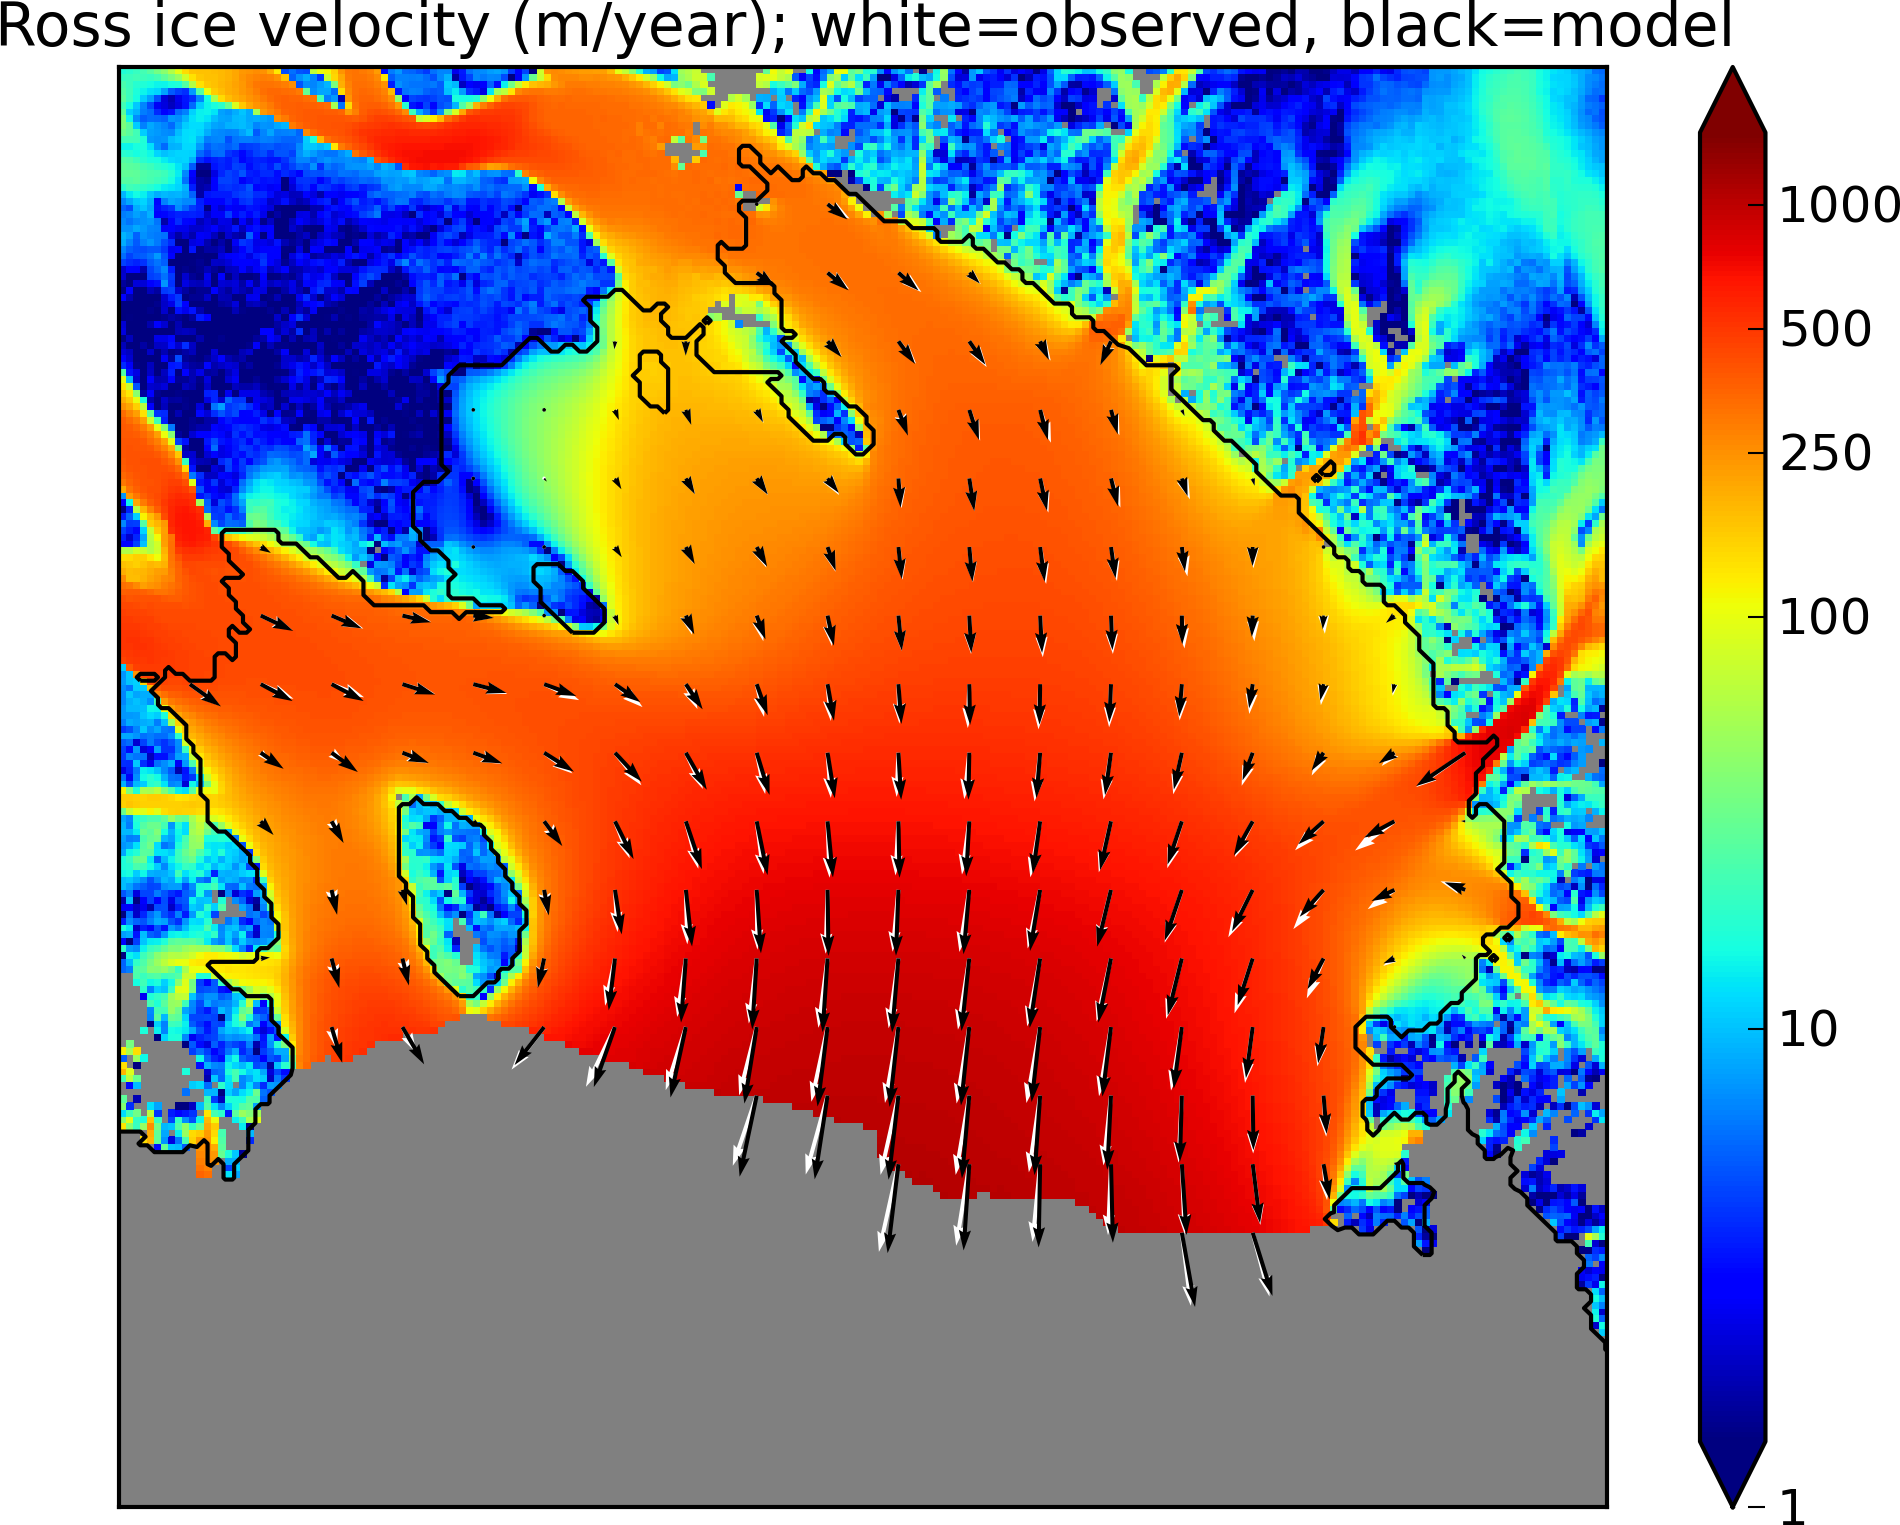
\includegraphics[width=3.5in,keepaspectratio=true]{rossquiver}
\end{center}

\vspace{.2in}

\begin{center}
\framebox{\parbox{5.0in}{ \emph{WARNING}:\index{PISM!warning}  PISM is an ongoing project.  Ice sheet modeling requires many choices.  Please don't trust the results of PISM or any other ice sheet model without a fair amount of exploration.  Also, please don't expect all your questions to be answered here.  Write to us with questions at \PISMEMAIL.} }
\end{center}


\clearpage\newpage

\section{Getting started}\label{sec:start}\index{PISM!getting started}

We get started with an extended example.  It applies PISM to model the Greenland ice sheet using data assembled by the \href{http://websrv.cs.umt.edu/isis/index.php/SeaRISE_Assessment}{Sea-level Response to Ice Sheet Evolution (SeaRISE)} group.  SeaRISE is a community-organized assessment process providing an upper bound on ice sheet contributions to sea level in the next 100--200 years, especially for the IPCC AR5 report in 2013.

The example in this section is a hands-on first look at PISM.  It is not an in-depth tutorial, and some details of what is happening will only be explained later.  Other sections list PISM options, discuss and help user's evaluate modeling choices, and explain the ways users will need to preprocess input data.

Some of the PISM output figures in this section were produced using a supercomputer.  But the basic run here can be done on a typical workstation or capable laptop.  That is why a rather coarse $20\,\textrm{km}$ grid is used in the main example in this section.  Of course PISM makes much higher spatial resolution possible by exploiting large-scale parallel processing.


To install PISM, see the Installation Manual at \href{http://www.pism-docs.org}{\texttt{www.pism-docs.org}}.
Once installed, executables \texttt{pismr} and \texttt{pclimate} should be available (i.e.~on your system's ``path''; confirm with ``\texttt{which pismr}'').  The instructions below also assume you are using a \texttt{bash} shell or one that accepts \texttt{bash} syntax.


\subsection{SeaRISE input data for the Greenland ice sheet}

The NetCDF data file which we use for input is freely-available online.  Descriptions of the data it contains, and a link to the file itself, are on this web page: 
\medskip

\centerline{\protect{\textbf{\url{http://websrv.cs.umt.edu/isis/index.php/Present_Day_Greenland}}}}
\medskip

\noindent The quickest way to get the file is to do
\begin{verbatim}
$ cd examples/searise-greenland
$ ./preprocess.sh
\end{verbatim}
\noindent The script \texttt{preprocess.sh}\footnote{\protect{This script requires \texttt{wget} and also NCO (NetCDF Operators; \url{http://nco.sourceforge.net/})}.} downloads the version 1.1 SeaRISE ``master'' present-day data set.  It adjusts the metadata in this file to make it PISM-readable.  In fact it creates several new NetCDF files which can be read by PISM; use \texttt{ncdump -h} to see their metadata.  Two of the new files contain famous time-dependent paleo-climate records from ice core and seabed core records; \texttt{pism_dT.nc} has GRIP while \texttt{pism_dSL.nc} has SPECMAP.

Also the preprocess script downloads the SeaRISE summary versions of IPCC AR4 (2007) climate projections, namely \texttt{ar4_precip_anomaly.nc} and \texttt{ar4_temp_anomaly.nc}.  These files are downloaded from \href{http://www.pism-docs.org/}{\texttt{www.pism-docs.org}}, but they are versions of the data at the SeaRISE page \url{http://websrv.cs.umt.edu/isis/index.php/Future_Climate_Data}.  These surface temperature and precipitation scenarios are used in the script \texttt{experiments.sh} to demonstrate offline coupling (forcing) in subsection \ref{subsect:forecastcaution} below.

Any of these NetCDF files can be viewed with \texttt{ncview} or other NetCDF visualization tools; see Table \ref{tab:NetCDFview} below.  An application of IDV to the master data set produced Figure \ref{fig:sr-input}, for example.

\begin{figure}[ht]
\centering
\mbox{\includegraphics[width=2.0in,keepaspectratio=true]{sr-greenland-thk}
  \qquad
  \includegraphics[width=2.0in,keepaspectratio=true]{sr-greenland-topg}
  \qquad
  \includegraphics[width=2.0in,keepaspectratio=true]{sr-greenland-prcp}}
\caption{The input present-day ice thickness (left; m), bedrock elevation (center; m), and present-day precipitation (right; m $\text{a}^{-1}$ ice equivalent) for SeaRISE-Greenland.  These are fields \texttt{thk}, \texttt{topg}, and \texttt{precipitation}, respectively, in file \texttt{pism_Greenland_5km_v1.1.nc} produced by running \texttt{preprocess.sh}.}
\label{fig:sr-input}
\end{figure}


\subsection{Run PISM}   \label{subsect:runscript}  We are ready to run PISM.  Like many Unix programs, PISM allows many command-line options.  Furthermore there are configuration parameters that get read from a file---see \mbox{\texttt{src/pism_config.cdl}} in the PISM source code.  Because PISM handles many different ice sheet, shelf, and glacier configurations, the list of user-configurable flags and parameters is quite long; for a complete list see \url{\PISMBROWSERURL}.  Therefore in practice we often build scripts to run PISM with the correct options, and we have done this for \mbox{SeaRISE-Greenland}.

Modeling ice sheets can be done by integrating paleo-climatic and long-time-scale information to build a model for the present state of the ice sheet, so our main script is called ``\texttt{spinup.sh}''.  The spin-up stage is the one which generally requires the most processor-hours, compared to a follow-on ``forecast'' stage.  To see what is done during spin-up, do this:
\begin{verbatim}
$ PISM_DO=echo ./spinup.sh |less
\end{verbatim}
Setting the environment variable \texttt{PISM_DO} in this way tells \texttt{spinup.sh} just to print out the commands it is about to run, not do them.\footnote{The script outputs more than a page so we pipe to \texttt{less}.  If you don't have \texttt{less}, try \texttt{more}.}

Note that ``\texttt{mpiexec -n 2 pismr}'' appears in the PISM runs done by \texttt{spinup.sh}.  This means that, by default in this script, the PISM executable \texttt{pismr} is run in parallel on two processes (e.g.~cores).  The executable name ``\texttt{pismr}'' stands for the standard ``run'' mode of PISM, in contrast to other, specialized modes described later.

For the rest of this example, we assume you have a workstation with 8 cores, but this example will work with 1 to 500 processes, with good scaling in speed.  The script takes the number of processes as its first argument (illustrated below).

The script \texttt{spinup.sh} starts by ``bootstrapping.''  This term describes the creation, by heuristics and simplified models, of the kind of full initial conditions needed for the evolving, time-dependent ice dynamics model.  In fact the first 100 model year run commanded by \texttt{spinup.sh} is this:
\small
\begin{verbatim}
mpiexec -n 8 pismr -config_override searise_config.nc -acab_cumulative \
  -skip -skip_max 10 -boot_file pism_Greenland_5km_v1.1.nc -Mx 76 -My 141 \
  -Lz 4000 -Lbz 2000 -Mz 101 -Mbz 11 -z_spacing equal \
  -atmosphere searise_greenland -surface pdd -ocean_kill \
  -y 100 -o g20km_pre100.nc
\end{verbatim}
\normalsize
The options describe a $76\times 141$ point grid in the horizontal, which gives 20 km grid spacing in both directions.  There are also important choices about the vertical extent and resolution of the computational grid; more on those later. 

Now, let's actually get the run going:
\begin{verbatim}
$ ./spinup.sh 8 >> out.spin20km &
\end{verbatim}
\noindent Because we have re-directed the text output, PISM will show what it is doing in the text file \texttt{out.spin20km} as it runs in the background.  Using \texttt{less} is a good way to watch such a growing text file.  Quickly the run will produce an early flow result in \texttt{g20km_pre100.nc}.

Soon after that some climatic boundary conditions sample results will appear in \texttt{g20km_climate-500a.nc}.  Such output from executable \texttt{pclimate} is effectively a movie of the stored and modeled climatic inputs provided to our ice dynamics model, including the results from surface models like the above-mentioned PDD model for surface mass balance.  This is a convenient way to, early in the modeling process, look at the critical surface mass balance and surface temperature inputs to the ice dynamics.


\subsection{Watching the spin-up}  \label{subsect:spinupsketch}  The next paragraphs describe what happens and what files are produced by the run which is underway.  We believe that the modeling choices represented here are reasonable, but they are not the only way to do it.  The user is encouraged to experiment; that is the point of a model!

After the completion of the first 100 model year run (\texttt{g20km_pre100.nc}), we then work to generate a more-physical enthalpy (i.e.~temperature and liquid fraction) field in which the modeled ice internal energy, its temperature, its softness, its stored basal water, and its basal melt rate are all in better balance with the ice sheet geometry and the simultaneously evolving flow velocity field.  Note the velocity advects the ice properties, especially enthalpy and thus ice softness.

The upper and lower surfaces of this modeled ice are held fixed at this stage.  The upper surface is held fixed by the option \texttt{-no_mass}, while the lower surface is held fixed in the sense that we do not yet apply a bed deformation model.  The resulting enthalpy field is in approximate equilibrium with a velocity field for which the surface kinematical equation \cite{Fowler} is unfortunately \emph{not} satisfied.  Also there is no sliding at this stage because good sliding requires good basal strength which requires good basal melt rates; these improve significantly as this no-sliding run evolves.

We sometimes call this early stage ``pre-spin-up'', a stage which follows on ``bootstrapping'' and comes before the classical paleo-climatic data-using ``spin-up''.  This ``pre-spin-up'' stage goes for 50,000 model years and yields the file \texttt{g20km_steady.nc} at the end.  Along the way the file \texttt{ex_g20km_steady.nc} is updated at every 500 model years, and it can be used to evaluate the degree to which we have reached a thermomechanically-coupled steady state.


\begin{figure}[ht]
\centering
%  temppabase from last time in ex_g10km_steady.nc and driving stress taud from g10km_SIA.nc
\mbox{\includegraphics[width=2.0in,keepaspectratio=true]{temppabase}
  \qquad \includegraphics[width=2.1in,keepaspectratio=true]{taud}}
\caption{Part of the model state at the beginning of paleo-climate-modeling ice sheet spin-up, in file \texttt{g20km_steady.nc} from running \texttt{spinup.sh}.  Left: pressure-adjusted basal temperature ($\phantom{|}^\circ$C; field \texttt{temp_pa}).  Right: driving stress magnitude $\rho g H |\grad h|$ (Pa; field \texttt{taud_mag}).}
\label{fig:sr-spinstart}
\end{figure}

The resulting model state in \texttt{g20km_steady.nc} is our model for the state of the Greenland ice sheet at the beginning of the paleo-climate record provided in the SeaRISE data set, namely 125,000 B.P.  There is, obviously, great uncertainty in this model for the distant past of the Greenland ice sheet.  Two views of the 10\,km model grid version of this state are in Figure \ref{fig:sr-spinstart}.

\begin{figure}[ht]
\centering
%  thk, cbase, csurf from g10km_0.nc
\mbox{\includegraphics[width=2.in,keepaspectratio=true]{thk}
  \qquad \includegraphics[width=2.in,keepaspectratio=true]{cbase}
  \qquad \includegraphics[width=2.in,keepaspectratio=true]{csurf}}
\caption{Model for the present-day Greenland ice sheet, based on spin-up over 125,000 model years using paleo-climate forcing.  Left: ice thickness (m).  Center: basal sliding speed (m/a).  Right: surface speed (m/a).  These are fields \texttt{thk}, \texttt{cbase}, and \texttt{csurf} from file \texttt{g10km_0.nc}.}
\label{fig:sr-spindone-map}
\end{figure}

The actual paleo-climate-driven spin-up starts from model state \texttt{g20km_steady.nc}.  We turn on three new mechanisms, climatic forcing, bed deformation, and improved stress balance.  There are two forms of climatic forcing. First, temperature offsets from GRIP core data affect the snow energy balance and thus rates of melting and runoff; the model is a simple temperature-index scheme described at the SeaRISE website.  Thereby the surface mass balance varies over time; in warm periods there is more marginal ablation.  Additionally, sea levels from the SPECMAP cores affects which ice is floating.

Significantly, we start using a more complete ice dynamics model with sliding controlled by a membrane stress balance, the SIA+SSA hybrid model described in section \ref{sec:dynamics}.  This is turned on with option ``\texttt{-ssa_sliding}''.  Also, we turn on a bed deformation model; the option is ``\texttt{-bed_def lc}''.  These options are discussed in section \ref{sec:modeling-choices}.  The command itself (do \verb|PISM_DO=echo ./spinup.sh 8| to see) is
\small
\begin{verbatim}
mpiexec -n 8 pismr -config_override searise_config.nc -acab_cumulative -skip -skip_max 10 \
  -i g20km_steady.nc -ssa_sliding -thk_eff -topg_to_phi 5.0,20.0,-300.0,700.0 -bed_def lc \
  -atmosphere searise_greenland,delta_T -surface pdd -paleo_precip pism_dT.nc \
  -atmosphere_delta_T_file pism_dT.nc \
  -ocean constant,delta_SL -ocean_delta_SL_file pism_dSL.nc -ocean_kill pism_Greenland_5km_v1.1.nc \
  -ts_file ts_g20km_m5000a.nc -ts_times -125000:yearly:-5000 -extra_file ex_g20km_m5000a.nc \
  -extra_vars ... -extra_times -125000:500:-5000 -ys -125000 -ye -5000 -o g20km_m5000a.nc
\end{verbatim}
\normalsize
but where the full list \verb|-extra_vars| is suppressed.  It uses option \verb|-i| for its input file \verb|g20km_steady.nc|, which is a PISM output file containing the grid information; contrast this with the earlier run which had options \verb|-boot_file| and specified a grid.   (A grid specification uses options \verb|-Mx|, \verb|-My|, \verb|-Mz|, etc.; see subsection \ref{subsect:grid}.)  This run command illustrates that PISM allows a great deal of command-line control, which is a desirable feature, but it also means in practice that most PISM modeling is done using shell scripts to run executables, as here.

This run goes from the SeaRISE-Greenland start time of -125,000 years to -5,000 years.  In this period, diagnostic outputs are written into \texttt{ex_g20km_m5000a.nc} at every 500 model years, and scalar time series including total ice volume are written into \texttt{ts_g20km_m5000a.nc} at every model year.  At the end of this period of the spinup we get the model state file \texttt{g20km_m5000a.nc}.  After that, a final run continues on the same grid from -5,000 years to present day, producing \texttt{g20km_0.nc}.  A variation on this last 5,000 model years run is put in \texttt{g20km_0_ftt.nc}.



The spun-up states \texttt{g20km_0.nc} or \texttt{g20km_0_ftt.nc} is intended to be a model for the Greenland ice sheet at the present day, and thus a basis on which to explore future ice sheet behavior.  If you run \texttt{./spinup N 2} then all of this is done on a 10\,km grid.  Figure \ref{fig:sr-spindone-map} shows some fields from the 10\,km model grid version of this present-day state.  The ice sheet thickness and surface velocity can be compared to present-day observations \cite{BKAJS}, and parameter dependences in the spin-up process should be explored.

Over the course of the spin-up we have saved the modeled ice volume in ``time-series'' NetCDF files.  This important model output can be viewed by
\begin{verbatim}
$ ncview ts_g20km_m5000a.nc ts_g20km_0.nc
\end{verbatim}
\noindent Figure \ref{fig:sr-spindone-ivolboth} shows this ice volume time series for the whole spin-up.  We see the modeled volatility of ice volume in the late ``Eemian'' period, between -120,000 and -115,000 BPE in the SeaRISE version of the GRIP temperature data.  We also see that the result \emph{does} depend on resolution.  Higher resolution grids allow the model to better resolve the flux through outlet glaciers especially, which are topographically-controlled, and such an effect explains the greater Eemian volume loss in the above 10\,km time series.  See the later examples in this manual for more on high resolution modeling.

\begin{figure}[ht]
\centering
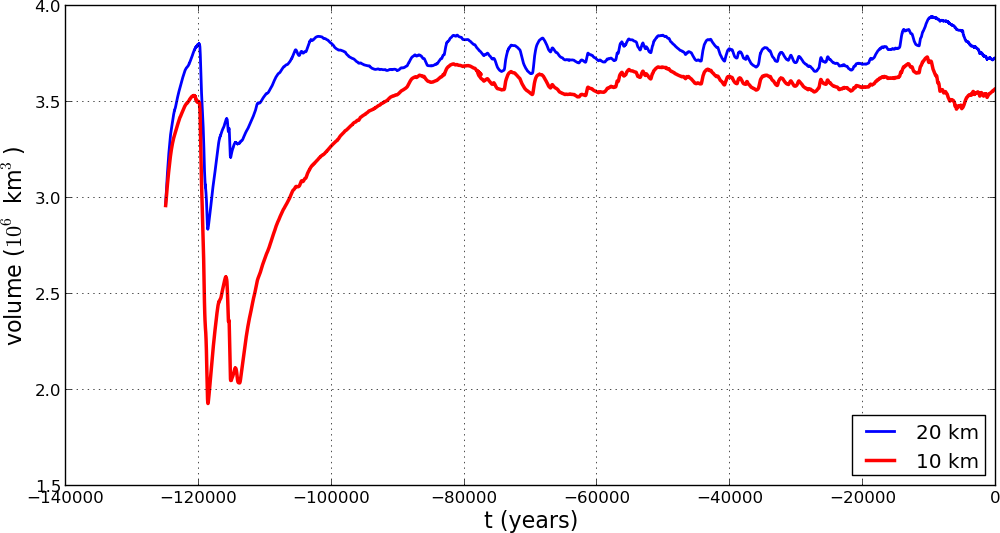
\includegraphics[width=4.5in,keepaspectratio=true]{ivolboth}
\caption{Time series of modeled ice sheet volume on 20km and 10km grids.}
\label{fig:sr-spindone-ivolboth}
\end{figure}

%from PISM0.4:  On an 8 core workstation the total run time for the complete 20\,km spin-up, which models 125,000 model years with ``full physics'' of the polythermal SIA+SSA hybrid type (section \ref{sec:dynamics}) is about 5 wall clock hours or 40 processor-hours.  For the same machine, the complete 10\,km spin-up used about 660 processor-hours, thus several wall-clock days.

On an the total run time for the complete 20\,km spin-up, which models 125,000 model years with ``full physics'' of the polythermal SIA+SSA hybrid type (section \ref{sec:dynamics}) is about 290 processor-hours.  The complete 10\,km spin-up used about 6131 processor-hours.

If done without membrane stresses (i.e.~non-sliding SIA only) these computational times are significantly reduced.  The polythermal versus ``cold'' energy-conservation choice corresponds to no performance difference of consequence.


\subsection{Going forward}  \label{subsect:forecastcaution}  In the same \verb|examples/searise-greenland| directory is a script \verb|experiments.sh|.  This does a suite of runs for 500 years into the future for the SeaRISE assessment, initializing from the above-computed modeled present-day state.  The first run is a ``control''  run assuming steady climate for the entire period.  Other runs perform the experiments described at \url{http://websrv.cs.umt.edu/isis/index.php/Category_1:_Whole_Ice_Sheet}.  Some runs use the AR4 climate forcing files which were produced when you ran \texttt{preprocess.sh}.  Once these runs are completed there are postprocessing scripts which primarily adjust metadata to match the standardizations used for the SeaRISE assessment.

Please run \verb|experiments.sh| and the postprocessing scripts, play with them, and modify them, but remember that we include these scripts for demonstration purposes.

Because real ice sheets, and ice sheet models too, have a ``memory'' of past climates, the results strongly depend on the nature of the spin-up process which preceded this ``forecast'' run.  Therefore, as already noted, it is critical to evaluate the quality of the spunup state, for example using present-day observations of surface velocity \cite{AschwandenAdalgeirsdottirKhroulev}, and other observations including ice temperature in ice bore-holes.  Critical thinking about a broad range of modeling hypotheses is prerequisite to building models of future behavior.


\subsection{Handling NetCDF files}\label{subsect:nctoolsintro}  At a superficial level, PISM is just a program which takes one or more NetCDF files as input, does some computation, and produces one or more NetCDF files as output.  As a result, the user needs tools to extract some meaning from the NetCDF output files and also, in the general case, more tools to create NetCDF files for input to PISM.\footnote{Regarding the creation of input files, see the section \ref{sec:bootstrapping-format} and table \ref{tab:modelhierarchy} for ideas about the data necessary for modeling.}

The most basic tools for converting NetCDF files to and from a standard text representation are called \texttt{ncdump} and \texttt{ncgen}.  A glance at Unix \texttt{man} pages for these tools might be wise at this time.

We most-regularly use \texttt{ncview} to look at NetCDF files.  Table \ref{tab:NetCDFview} lists NetCDF tools that can be useful for visualizing and post-processing PISM output files, as well as for preparing input data.  We find \texttt{ncview}, NCO, IDV and PyNGL especially useful.

\newcommand{\netcdftool}[1]{#1\index{NetCDF!tools!#1}}
\begin{table}[ht]
\centering
\small
\begin{tabular}{llp{0.4\linewidth}}
  \toprule
  \textbf{Tool} & \textbf{Site} & \textbf{Function} \\
  \midrule
  \netcdftool{\texttt{ncdump}} & \emph{included with any NetCDF distribution} & dump binary NetCDF as \texttt{.cdl} (text) file \\
  \netcdftool{\texttt{ncgen}} & \emph{included with any NetCDF distribution} & convert \texttt{.cdl} file to binary NetCDF \\
  \netcdftool{\texttt{ncview}} & \href{http://meteora.ucsd.edu/~pierce/ncview_home_page.html}{\texttt{meteora.ucsd.edu/~pierce/ncview_home_page.html}} & quick graphical view \\
  \netcdftool{IDV} & \url{http://www.unidata.ucar.edu/software/idv/} & more complete visualization \\
  % \netcdftool{Paraview} & \href{http://www.paraview.org}{\texttt{www.paraview.org}} & powerful open-source parallel visualization \\
  \netcdftool{NCL} &  \url{http://www.ncl.ucar.edu} & NCAR Command Language\\
  \netcdftool{PyNGL} &  \url{http://www.pyngl.ucar.edu} & Python version of NCL\\
  % \netcdftool{VisIt} & \href{http://visit.llnl.gov}{\texttt{visit.llnl.gov}} & advanced parallel visualization \\
  \netcdftool{NCO}\index{NCO (NetCDF Operators)} & \url{http://nco.sourceforge.net/} & NetCDF Operators; command-line tools\\
  \netcdftool{CDO} & \url{http://code.zmaw.de/projects/cdo} & Climate Data Operators; more command-line tools, including conservative re-mapping \\
  & \url{www.unidata.ucar.edu/software/netcdf/} & root for NetCDF information \\
  \bottomrule
\end{tabular}
\normalsize
\label{tab:NetCDFview}
\caption{Tools for viewing and modifying NetCDF files.}
\end{table}


%%% Local Variables: 
%%% mode: latex
%%% TeX-master: "manual"
%%% End: 


% LocalWords:  metadata SPECMAP paleo html IDV



\clearpage
\newpage
\section{Ice dynamics, the PISM view}\label{sec:dynamics}

\subsection{PISM design principles}\index{PISM!principles}  This section gives an overview of ice dynamics models in PISM.  First, some organizing principles:
\begin{enumerate}
\item source code should be open, free, and work well with other free software tools,
\item science is better with publicly-available data,
\item numerical methods should be verifiable (comparable to exact solutions of the equations),
\item shallow models are the most effective at whole ice sheet scale,
\item everything computed diagnostically (instantaneously) should be available prognostically (can evolve in time), and
\item climate inputs should affect ice dynamics by a well-defined interface.
\end{enumerate}

\noindent We do not claim to follow these principles perfectly, but principle 1 is illustrated by our existence and principle 2 by examples in sections \ref{sec:start}, and \ref{sec:ross}.  Principle 3 is addressed in section \ref{sec:verif}.  Principles 4, 5, and 6 are addressed next.


\subsection{Two main shallow models, SIA and SSA}\index{PISM!SIA}\index{PISM!SSA}  At each time-step of a typical PISM run, the geometry, temperature, and basal strength of the ice sheet are included into stress (momentum) balance equations to determine the velocity of the flowing ice.   The ``full'' stress balance equations, namely the (non-Newtonian) Stokes model for slowly-flowing fluids \cite{Fowler}, are themselves an inertia-free approximation of the conservation of momentum equations.  Even though PISM does not solve this ``full'' model, it can numerically solve two different shallow approximations which are suited to the situations in large ice sheet and ice shelf systems:
\begin{itemize}
\item the non-sliding shallow ice approximation (SIA)\index{SIA (shallow ice approximation)} \cite{Hutter}, also called the ``lubrication approximation'' \cite{Fowler}, which describes ice as flowing by shear in planes parallel to the geoid, with a strong contact of ice base to bedrock, and
\item the shallow shelf approximation (SSA)\index{SSA (shallow shelf approximation)} \cite{WeisGreveHutter}, which describes a membrane-type flow of floating ice \cite{Morland}, or grounded ice which is sliding over a weak base \cite{MacAyeal,SchoofStream}.
\end{itemize}
PISM solves both the SIA and SSA equations in parallel.  Time-stepping solutions of the mass continuity and energy conservation equations are possible when using each model.

The SIA\index{SIA (shallow ice approximation)!applicability} equations are, as a rule, easier and quicker to numerically solve than the SSA, and they are also easier to parallelize.\index{parallelization!relative ease of, between SIA and SSA}  They describe the shear as a local function of the driving stress of classical glaciology \cite{Paterson}.  They can confidently be applied to those grounded parts of ice sheets for which the basal ice is frozen to the bedrock, or minimally sliding, and for which the bed topography is relatively slowly-varying in the map-plane \cite{Fowler}.  These characteristics apply to the majority \emph{by area} of the Greenland and Antarctic ice sheets.  We recommend solving the SIA with a completely \emph{non-sliding} base because the ad~hoc addition of ``sliding laws''\index{SIA (shallow ice approximation)!sliding laws} into the SIA stress balance, and especially schemes which ``switch on'' at the pressure-melting temperature \cite{EISMINT00}, have bad continuum and numerical modeling consequences \cite[appendix B]{BBssasliding}.

The SSA\index{SSA (shallow shelf approximation)!applicability} equations, by contrast, can confidently be applied to large floating ice shelves, which have small depth-to-width ratio and negligible basal resistance \cite{Morland,MorlandZainuddin}.  The flow speeds in ice shelves are frequently an order-of-magnitude higher than in the non-sliding, grounded parts of ice sheets, and this speed contrast is easily seen in comparing the solutions of SIA and SSA models.

Terrestrial ice sheets also have fast-flowing grounded parts, however, called ``ice streams'' or ``outlet glaciers'' \cite{TrufferEchelmeyer}.  Such features appear at the margin of, and sometimes well into the interior of, the Greenland \cite{Joughinetal2001}\index{Ice Sheets!Greenland ice sheet} and Antarctic \cite{BamberVaughanJoughin}\index{Ice Sheets!Antarctic ice sheet} ice sheets.  Describing these faster-flowing grounded parts of ice sheets requires, at least, something more than the non-sliding SIA because adjacent columns of ice which have different amounts of basal resistance exert strong ``longitudinal'' or ``membrane'' stresses \cite{SchoofStream} on each other.  One might use the full Stokes equations, or a ``higher-order'' model (which still uses some shallow approximations \cite{Blatter,Pattyn03}), but this immediately leads to a resolution-versus-stress-inclusion tradeoff because the amount of computation per map-plane grid location is so much higher in these models.  Also, with any stress balance model one must still specify an appropriate sliding boundary condition, and uncertainty in this boundary condition may (and usually does) dominate the modeling error made by not including higher-order stresses in the balance.

If the fast-flowing grounded ice is sufficiently shallow, in the usual aspect-ratio sense, then the SSA model can be applied.  The best-known combination of the SSA model with a choice of basal resistance model is the Siple Coast (Antarctica) ice stream model by MacAyeal\index{People!MacAyeal, Doug} \cite{MacAyeal}, who used a linearly-viscous model for the underlying till.  A free boundary problem with the same (SSA) balance equations is the Schoof\index{People!Schoof, Christian} \cite{SchoofStream} model of ice streams, using a plastic (Coulomb) sliding relation.  In this model ice streams appear where there is ``till failure'' \cite{Paterson}---the basal shear stress exceeds the yield stress imposed as a boundary condition---and the location of ice streams is not imposed in advance.

As noted, both the SIA and SSA models are \emph{shallow} approximations.  More precisely, these model equations are derived from the Stokes equations by different small-parameter arguments, both based on a small depth-to-width ratio for the ice sheet.  Both models, and ``higher order'' models as well, approximate the pressure as hydrostatic.  For the small-parameter argument in the SIA case see \cite{Fowler}.  For the corresponding SSA argument, see \cite{WeisGreveHutter} or the appendices of \cite{SchoofStream}.  Schoof and Hindmarsh \cite{SchoofHindmarsh} have analyzed the connections between these shallowest models and ``higher order'' models, while \cite{GreveBlatter2009} discusses ice dynamics and stress balances comprehensively.

In PISM the SSA may be used as a ``sliding law'' for grounded ice which is already modeled everywhere by the non-sliding SIA \cite{BBssasliding}.  In brief, our concept for grounded ice is that, in addition to including shear in planes parallel to the geiod, we must balance the membrane stresses which become important anywhere there is significant sliding, and this inclusion is especially important when there are changes in basal strength, both spatial and temporal.  The more traditional use of ``sliding laws'' in pure-SIA models does not incorporate this basic physical truth \cite{Fowler01}.

The resulting ``SIA+SSA hybrid'' model is recommended by the PISM developers for most whole ice sheet modeling purposes because it seems to be a good compromise given currently available data and computational power (see \cite{BKAJS,Martinetal2011,Winkelmannetal2011}, for example).  This ``sliding law'' role for the SSA is in addition to its more obvious role in ice \emph{shelf} modeling, and so the SSA plays both roles in a PISM whole ice sheet model if there are large floating ice shelves--- as in Antarctica \cite{Martinetal2011,Winkelmannetal2011}.

By default, PISM does not numerically solve the SSA because any such solution must go with a conscious user choice about basal strength.  The user must both use a command-line option to turn on the SSA (section \ref{subsect:ssacontrol}) and also make choices in input files and runtime options about basal strength (section \ref{subsect:basestrength}).


\subsection{A hierarchy of simplifying assumptions for grounded ice flow}
\label{sec:model-hierarchy}\index{PISM!hierarchy of simplifying assumptions}

Table \ref{tab:modelhierarchy} describes a hierarchy of models, listed in order of increasing effectiveness in modeling grounded ice sheets with fast flow features.  This is also the order of increasing need for data to serve as boundary and initial conditions, an important consideration for the scientific user.

As an additional row for such a table, one might list ``full Stokes''.  That stress balance is \emph{not} planned for PISM at any time, however, as its numerical solution requires a fundamentally different computational architecture.

It makes sense to also talk about an \emph{ice shelf} model hierarchy, and even about a special hierarchy of models for the transition from grounded to floating ice \cite{SchoofMarine1}, but this would take us too far afield.  Currently, ice shelves should always be modeled by the SSA equations in PISM.  See section \ref{sec:ross}.

Although it begins to expose the internals of PISM, we think it is also helpful to see the implemented stress balances as PISM software components (C++ classes).  Figure \ref{fig:stressbalance} shows that the sequence of actions taken by SIA-only, SSA-only, and SIA+SSA hybrid models is, in some sense, the same: a membrane stress solution first, a distribution of vertical shear in the column of ice second, and a use of incompressibility to compute the vertical component of the velocity third.  The nonsliding SIA-only model has a degenerate first step and the SSA-only model has a degenerate second step.  The hybrid model described by Pollard and deConto \cite{PollardDeConto}, for another example, would add the shear in the column in a different manner (than in the current implementation, following \cite{BBssasliding,Winkelmannetal2011}).

\newenvironment{tightlist}{\begin{itemize}  \vspace{-0.15in}\addtolength{\itemsep}{-0.5\baselineskip} } {\vspace{-0.1in} \end{itemize}}

%\newcommand{\nolist}[1]{\begin{tightlist} \item[] [\emph{#1}] \end{tightlist}}
\newcommand{\nolist}[1]{[\emph{#1}] \vspace{0.1in}}

\begin{table}[ht]
\small\medskip
\begin{tabular}{p{0.22\linewidth}p{0.40\linewidth}p{0.32\linewidth}}
\toprule
\textbf{Model} & \textbf{Assumptions} & \textbf{Required data} \\
\midrule
\vspace{2mm}  \emph{perfectly-plastic ice} \small & \vspace{2mm}\emph{steady state}; ice has shear stresses at or below a pre-determined ``yield stress''; requires location of ice sheet margin  \vspace{2mm} & \vspace{2mm} \begin{tightlist} \item bed elevation\end{tightlist} \\
\emph{balance velocities} \small & \emph{steady state}; ice flows down surface gradient \cite{JoughinetalGrBal97} & \nolist{same as above, plus:}  \begin{tightlist} \item surface mass balance \item initial ice thickness \end{tightlist} \\
\textsc{isothermal SIA} & non-sliding lubrication flow, fixed softness \cite{BLKCB,EISMINT96} & \nolist{same as above, but time-dependence is allowed} \\
\textsc{thermo-coupled SIA} & non-sliding lubrication flow, temperature-dependent softness \cite{BBL,EISMINT00} & \nolist{same as above, plus:} \begin{tightlist} \item surface temperature \item geothermal flux \end{tightlist} \\
\textsc{polythermal SIA} & same, but allowing $>0$ liquid water in temperate ice; conserves energy better \cite{AschwandenBuelerKhroulevBlatter,Greve} \vspace{2mm} & \nolist{same as above} \\
\textsc{SIA + SSA hybrid} & SSA as a sliding law for thermo-coupled SIA \cite{BBssasliding}; polythermal is the default & \nolist{same as above, plus:} \begin{tightlist} \item basal layer (``till'') strength \end{tightlist} \\
\emph{Blatter-Pattyn} \small & ``higher-order'', bridging stresses \cite{Blatter,Pattyn03,SchoofCoulombBlatter} & \nolist{same as above} \\
\bottomrule
\end{tabular}
\normalsize
\label{tab:modelhierarchy}
\caption{Hierarchy of current and planned flow models in PISM, for the grounded
  parts of ice sheets, from most to fewest simplifying assumptions \emph{and}
  from least to greatest need for boundary data.  The \emph{italicized} models
  are planned for future versions of PISM but are not implemented so far..}
\end{table}


\subsection{Evolutionary and diagnostic modeling} \label{subsect:basicmodes}\index{PISM!evolution run}\index{PISM!diagnostic run}    The main goal of a numerical ice sheet model like PISM is to be a dynamical system which evolves over time as similarly as possible to the modeled ice sheet.  Such a goal assumes one has the right climate inputs and parameter choices at each time step.  For predictive purposes, it also assumes one has the right initial conditions, adequately describing the present state of the ice sheet.  This last assumption is rarely satisfied.  Instead, heuristics must be used to minimally-initialize an ice sheet model, before a possible stage of paleo-climate driven spin-up; see section \ref{sec:boot}.

Underlying an ice sheet model like PISM are evolution-in-time partial differential equations.  PISM solves these by taking small time steps.  ``Small'' time steps vary from hundredths to many model years, depending primarily on grid resolution and modeled ice flow speed.  Time steps are chosen adaptively in PISM, according to the stability criteria of the several numerical methods.

However, much ice flow modeling, especially of streams and shelves, uses only instantaneous ``diagnostic'' solution of the partial differential equations which determine the velocity field.  The models in PISM can produce such ``instantaneous'' velocity fields because of the slowness of the ice, in the sense that inertia can be neglected in the stress balance \cite{Fowler}.  The goal of a ``diagnostic run'' is usually to compute this velocity field, especially its observable surface values.  For example, a diagnostic run might be the ``forward model'' step in inverting surface velocities for basal strength\dots but that is beyond the scope of this \emph{Manual}.

Sections \ref{sec:start} and \ref{sec:ross} are examples illustrating evolutionary and diagnostic modeling modes of PISM.  The first of these describes time-stepping evolution models for the Greenland ice sheet, while the second describes a diagnostic SSA model for the Ross ice shelf.


\begin{figure}
  \centering
  \includegraphics[width=6in]{stressbalance}
  \caption{The SIA-only, SSA-only, and SIA+SSA hybrid models represent different ``routes'' through stress balance PISM components.  In each case the inputs are ice geometry and boundary stresses, and the final output is a three-dimensional velocity field within the ice.}
  \label{fig:stressbalance}
\end{figure}


\subsection{Climate inputs, and their interface with ice dynamics}
\label{sec:climate-inputs}  

Because PISM's job is to approximate ice flow, its ``world view'' is centered around ice dynamics.  The discussion of boundary conditions, in this \emph{Manual} is necessarily ``ice-centric'' in our description here, but there is no constraint on the nature of, or completeness of, climate models which could be coupled to PISM.  This section applies the PISM organizing principle above (section \ref{sec:dynamics}): \emph{climate inputs affect ice dynamics by a well-defined interface}.

Figure~\ref{fig:climate-inputs} illustrates that any PISM ice sheet model has an interface (green) to a surface processes layer containing snow, firn, and liquid (or refrozen) runoff, and to the ocean (blue) if there is floating ice.  The surface processes layer might be very simple.  If it is ``owned'' by the PISM model then there is an additional interface (red) to the atmosphere above.  The interface to the surface layer is assumed in PISM to cover the whole surface of the ice, including ablation areas and even ice-free land.  Table \ref{tab:ice-dynamics-bc} lists fields which are needed as boundary conditions at the interfaces.

\begin{figure}
  \centering
  \includegraphics[width=6in]{figs/climate-cartoon.pdf}
  \caption{PISM's view of interfaces between an ice sheet and the outside world}
  \label{fig:climate-inputs}
\end{figure}

\begin{table}[h]
  \centering
 \begin{tabular}{p{0.35\linewidth}p{0.55\linewidth}}
    \toprule
    \textbf{Boundary} & \textbf{Necessary conditions}\\
    \midrule
    Top ice surface (below firn) (\textcolor{green}{green})& Ice temperature (or enthalpy) and mass flux into the ice\\
    Bottom surface of the thermal bed layer (not shown) & Geothermal flux\\
    Ice shelf basal surface (\textcolor{blue}{blue})& Mass flux into the ocean and ice boundary temperature\\
   \bottomrule
  \end{tabular}
\caption{Boundary conditions required by PISM's ice dynamics core; see figure \ref{fig:climate-inputs}}
\label{tab:ice-dynamics-bc}
\end{table}

Regarding the base of the ice, as described in section \ref{subsect:beddef} PISM also includes an optional bed deformation component approximating the movement of the Earth's crust and upper mantle in response to changing ice load.   Furthermore the temperature of the layer of bedrock in contact with grounded ice is included in the conservation of energy model.  In this sense everything below the black dashed line (i.e.~ice and bedrock) is ``owned'' by PISM.  This fact adds two more boundary interfaces for the ice dynamics core: sub-ice-shelf/ocean (shown in blue) and the bottom of the bedrock thermal layer (not shown).

The PISM ice dynamics core would like to be able to get fields listed in Table
\ref{tab:ice-dynamics-bc} directly from observations or measurements, or directly from a GCM.  In many realistic modeling situations, however, PISM code must be used for all or part of the surface processes modeling necessary to provide the ice-dynamics core with the ``right'' fields.  Due to differences in model resolutions and required down-scaling, this need for some PISM-based boundary-processes modeling includes cases where PISM is coupled to a GCM.  In the kind of ``offline'' runs described in this \emph{Manual}, boundary processes are modeled, even if trivially.

Thus, to be able to use the data that \emph{is} available, an ice-sheet model has to
have additional components that are responsible for modeling surface (snow)
processes or sub-shelf/ocean interaction.  These components might be very minimal, merely turning data that we already have into data in the right units and with the right metadata, so that PISM knows what to do with it, for example.

Thus we have PISM's design: the ice-dynamics-and-earth-deformation PISM
core does not contain any parameterization or other model for boundary mass or
energy balance.  These boundary parameterizations and models are present in the PISM source code, however, as instances of \emph{PISMComponent} classes.  This simplifies customizing and debugging PISM's climate
inputs, promotes code reuse.  Moreover, it isolates the code that needs to be changed to
couple PISM to a climate model.

Users wishing to customize PISM's climate inputs should see the \emph{PISM
  Source Browser} at
\begin{quote}
  \url{\PISMBROWSERURL}
\end{quote}
 and the documentation
of \mbox{\emph{PISMSurfaceModel}}, \mbox{\emph{PISMAtmosphereModel}}, and
\mbox{\emph{PISMOceanModel}} therein.  Also, section \ref{sec:start} describes a
modeling example using a non-standard air temperature parameterization. Looking
at the file
\begin{quote}
\texttt{src/coupler/atmosphere/PAEismintGreenland.cc}
\end{quote}
may be a reasonable start.

Note that figure~\ref{fig:climate-inputs} includes an interface between the surface layer and the air (red dashed line).
Unlike the ones listed in table~\ref{tab:ice-dynamics-bc}, this interface
\emph{may not even be present in some PISM configurations:} the ice dynamics
core of PISM only ``knows'' about mediums bordering ice and bedrock. A pair
consisting of a \emph{PISMSurfaceModel} and a \emph{PISMOceanModel} may be
hiding anything from a nearly trivial parameterization of ice surface
temperature plus surface and sub-shelf mass fluxes to a GCM of great
complexity.

Figure~\ref{fig:climate-input-data-flow} illustrates the corresponding data
flow \emph{into} the PISM core; the data flow in the other direction depends on
particular modeling choices.

This figure requires an explanation: a ``modifier'' in this context is an
adjustment of climate inputs that can be used with different climate
choices.  Using ice-core-derived air temperature offsets to model the
space-time distribution of paleo surface temperature is an example.  Note that
PISM has a generic ``forcing'' mechanism that can be paired with another model.
Please see the \emph{PISM's climate forcing components} document for
a list of climate components included in PISM source code and other details.

\begin{figure}
  \centering
  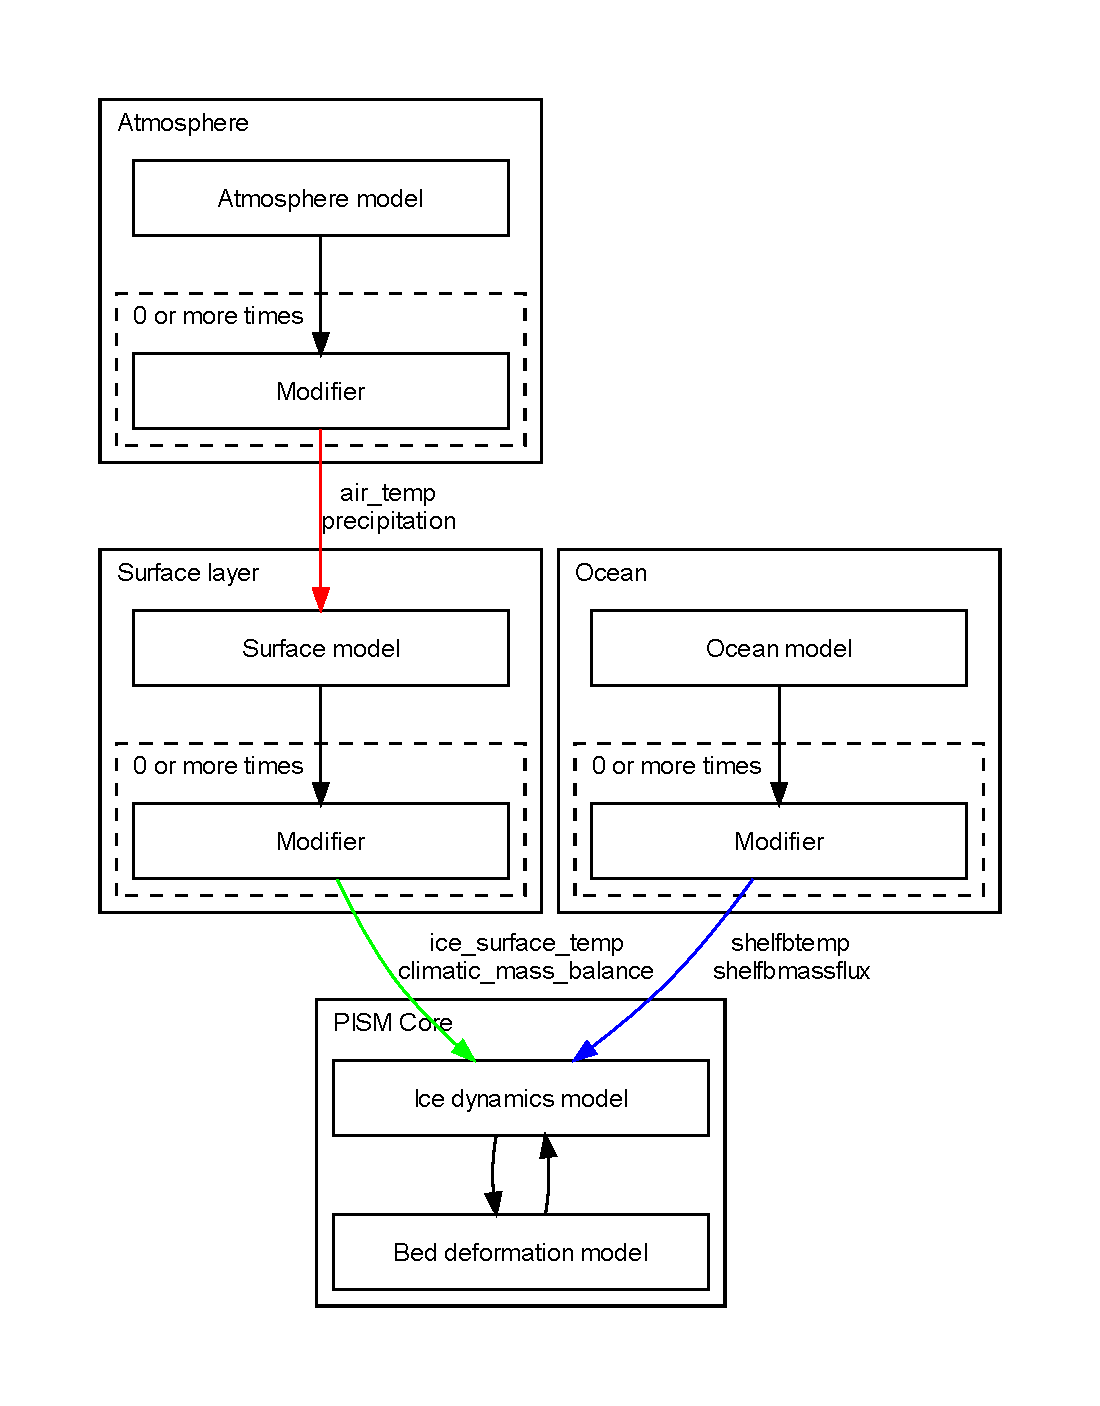
\includegraphics[width=5in]{figs/data-flow.pdf}
  \caption{PISM climate input data flow. Colored arrows correspond to interfaces in
    figure \ref{fig:climate-inputs}.}
  \label{fig:climate-input-data-flow}
\end{figure}

Why describe this structure here? On the one hand, some users may be interested
in coupling PISM to other models. On the other hand, the PISM authors do not
claim expertise in modeling atmosphere, ocean, or even snow processes.   So the
separation has a code-reliability purpose. Indeed PISM users need to know that
they are ultimately responsible for providing the climate inputs they intend.
The auxiliary tool \texttt{pclimate}, also described in \emph{PISM's climate
  forcing components}, is intended to help users observe the climate inputs
they have chosen, without involving ice dynamics at all.


\clearpage
\newpage
\section{Initialization and bootstrapping}
\label{sec:boot}

There are three ways to start PISM,\begin{itemize}
\item the executables \texttt{pisms} and \texttt{pismv} initialize simplified-geometry experiments and verification tests, respectively, from formulas in the source code,
\item \texttt{-i} reads a previously-saved PISM model state, a NetCDF file, and
\item \texttt{-boot_file} reads an ``incomplete'' NetCDF file and uses heuristics to fill in needed fields.
\end{itemize}
Realistic modeling usually starts with the \texttt{-boot_file} option because real ice sheet observations are never complete initial conditions for ice sheet models.

\subsection{Initialization from a saved model state}  ``Initialization''\index{initialization!from saved model state} has a specific, simple meaning in PISM.  If a previous PISM run has saved a NetCDF file using ``\texttt{-o}'' then that file will contain complete initial conditions for continuing the run.  The output file from the last run can be loaded with ``\texttt{-i}'': \index{executables!\texttt{pisms}}

\begin{verbatim}
$ pisms -eisII A -y 100 -o foo.nc
$ pisms -eisII A -i foo.nc -y 100 -o bar.nc
\end{verbatim}
\smallskip

Note that simplified-geometry experiments (section \ref{sec:simp}) and verification tests (section \ref{sec:verif}) do not need input files at all because they initialize from formulas in the source code.  They can be continued from saved model states using \texttt{-i}.  As in the above example, however, specifying the simplified geometry experiment or verification test \emph{is} necessary, so that the run can continue with the climate inputs for that experiment or test.  For example, based on the above \texttt{pisms} runs, it is valid to do
\begin{verbatim}
$ pismr -i foo.nc -y 100 -o bar.nc ...
\end{verbatim}
but the climate and other parameters use PISM default values, and thus are not (necessarily) the values specified in EISMINT II.

As a technical but important note about saved states, a PISM run with \texttt{-ssa_floating_only} or \texttt{-ssa_sliding}
also saves the last SSA velocities to the output file, in variables 
\texttt{u_ssa} and \texttt{v_ssa}. The presence
of these velocities adds efficiency in restarting.  If you want a PISM restart to
ignore these velocities use \texttt{-dontreadSSAvels}.

\subsubsection*{\texttt{-i} file format}
\label{sec:i-format}
PISM produces\footnote{Or, more accurately, attempts to produce; please let us know about violations you come across.} CF-1.5 compliant NetCDF\index{PISM!NetCDF file format}\index{NetCDF} files.  The easiest way to learn the output format \emph{and} the \texttt{-i} format is to do a simple run and then look at the metadata in the resulting file, like this:
\begin{verbatim}
$ pisms -eisII A -y 10 -o foo.nc
$ ncdump -h foo.nc | less
\end{verbatim}

Note that variables have a \texttt{pism_intent}\index{PISM!\texttt{pism_intent} attribute} attribute.  When that attribute is \texttt{diagnostic}, the variable can be deleted from the file without affecting whether PISM can use it as a \texttt{-i} input file.  Variables with \texttt{pism_intent} = \texttt{model_state}, by contrast, must be present for use with \texttt{-i}.

Regarding the automatically produced time variable, which has a \texttt{units} attribute like \texttt{"seconds since 1-1-1"}, note that CF metadata conventions require using a reference date in the units string of a time (\texttt{time}) variable. By default PISM ignores this reference date.


\subsection{Bootstrapping}
\label{sec:bootstrapping}
\optsection{Bootstrapping}
\optseealso{Grid}

``Bootstrapping''\index{bootstrapping}\index{initialization!by bootstrapping} in PISM means starting a modeling run with less than sufficient data, and letting the model fill in needed values according to heuristics.  These heuristics are applied before the first time step is taken, so they are part of an initialization process.  Bootstrapping uses the option \fileopt{boot_file}.

The need for an identified stage like ``bootstrapping'' comes from the fact that initial conditions, for the evolution equations describing an ice sheet, are not typically observable.  As a principal example of this problem, these equations require the temperature within the ice at the time the run is started.  Glaciological observations, specifically remote-sensed observations which cover a large fraction or all of an ice sheet, never include this temperature field in practice.

Instead, evolutionary ice sheet modeling necessarily does something like this
to get ``reasonable'' initial fields within the ice:
\begin{enumerate}
\item start only with observable quantities like surface elevation, ice thickness, and ice surface temperature,
\item ``bootstrap'' as defined here, using heuristics to fill in temperatures at depth and to give a preliminary estimate of the basal sliding condition, and thus of the three-dimensional velocity field, and
\item \emph{either} do a long run holding the current geometry and surface temperature steady,  to evolve toward a ``more physical'' steady state which will have compatible temperature field, velocities, and age field,
\item \emph{or} do a long run using an additional spatially-imprecise historical record from an ice core or a sea bed core (or both), to apply forcing to the surface temperature or sea level (for instance), but with the same functional result of filling in a temperature, velocity, and age.
\end{enumerate}

The heuristics used by PISM are, for now, only documented in the source code file \texttt{src/base/iMbootstrap.cc}.

When using \fileopt{boot_file} you will need to specify both grid dimensions (using \texttt{-Mx}, \texttt{-My} and \texttt{-Mz}) and the height of the computational box for the ice with \texttt{-Lz}.  The data read from the file can determine the horizontal extent of the model, if options \texttt{-Lx}, \texttt{-Ly} are not set.  The additional specification of vertical extent by \texttt{-Lz} is reasonably natural because realistic data used in ``bootstrapping'' are two-dimensional.  Not specifying all four options \texttt{-Mx}, \texttt{-My}, \texttt{-Mz}, \texttt{-Lz} \emph{when bootstrapping with} \texttt{-boot_file} is an error.

If \texttt{-Lx} and \texttt{-Ly} specify horizontal grid dimensions smaller than in the bootstrapping file, PISM will cut out the \emph{center} portion of the domain. Options \intextoption{x_range} and \intextoption{y_range} each take a list of two numbers, a list of minimum and maximum $x$ and $y$ coordinates, respectively (in meters). This makes it possible to select a subset that is not in the center of a bootstrapping file grid.

\subsubsection*{\texttt{-boot_file} file format}
\label{sec:bootstrapping-format}

Allowed formats for a bootstrapping file are relatively simple to describe. 
\begin{enumerate}
\item NetCDF variables should have the \texttt{units} containing a
  UDUNITS-compatible string. If this attribute is missing, PISM will assume
  that a field uses MKS units.\footnote{PISM uses a library called UDUNITS\index{PISM!uses UDUNITS when reading NetCDF files}\index{UDUNITS} to convert data present in an input file to MKS.   This means that having ice thickness in feet or kilometers, or temperature in Celsius for example, is allowed.}
\item NetCDF coordinate variables should have \texttt{standard_name} or
  \texttt{axis} attributes. These are used to
  determine which \emph{spatial} dimension a NetCDF dimension corresponds to;
  please see a \texttt{ncdump -h} output from a file produced by PISM for an example. (This implies
  that \texttt{x} and \texttt{y} dimensions need not be called ``\texttt{x}''
  and ``\texttt{y}''.
\item Coordinate variables have to be strictly increasing.
\item All three-dimensional variables will be ignored in bootstrapping.
\item The \texttt{standard_name} attribute is used to identify a variable, so
  the variable names need not match corresponding variables in a
  PISM output file. Please see \url{\PISMBROWSERURL} for a list of CF standard
  names used in PISM.
\item Any two-dimensional variable except bed topography and ice thickness may
  be missing. For those missing variables some heuristic will be applied. See
  table \ref{tab:modelhierarchy} for a sketch of the data necessary for
  bootstrapping, and \texttt{src/base/iMbootstrap.cc} for all further details.
\item Surface elevation is ignored if present. Users with surface elevation and
  bed elevation data should produce an ice thickness variable, with
  \texttt{standard_name} = \texttt{land_ice_thickness} for bootstrapping. The
  bed elevation (topography) is read by \texttt{standard_name} =
  \texttt{bedrock_altitude}.
\end{enumerate}


\clearpage\newpage

\section{Making Modeling Choices}
\label{sec:modeling-choices}

\subsection{Computational box} \label{subsect:coords}
\optsection{Computational box}
\optseealso{Grid}

PISM does all simulations in a computational box\index{PISM!computational box} which is rectangular in the PISM coordinates.

The coordinate system has horizontal coordinates $x,y$ and a vertical coordinate $z$.  The $z$ coordinate is measured positive upward from the base of the ice and it is exactly opposite to the vector of gravity.  The surface $z=0$ is the base of the ice, however, and thus is usually not horizontal in the sense of being parallel to the geoid.   The surface $z=0$ is the base of the ice both when the ice is grounded and when the ice is floating.

Bed topography is, of course, allowed.  In fact, when the ice is grounded, the true physical vertical coordinate $z'$, namely the coordinate measure relative to a reference geoid, is given by $z'=z+b(x,y)$ where $b(x,y)$ is the bed topography.  The surface $z'=h(x,y)$ is the surface of the ice.

In the grounded case the equation $h(x,y)=H(x,y)+b(x,y)$ always applies if $H(x,y)$ is the thickness of the ice.  In the floating case, the physical vertical coordinate is $z'=z-(\rho_i/\rho_s) H(x,y)$ where $\rho_i$ is the density of ice and $\rho_s$ the density of sea water.  Again $z=0$ is the base of the ice, which is the surface $z' = -(\rho_i/\rho_s) H(x,y)$.  The surface of the ice is $h(x,y) = (1-\rho_i/\rho_s) H(x,y)$.  All we know about the bed elevations is that they are below the base of the ice when the ice is floating.  That is, the \emph{flotation criterion} $-(\rho_i/\rho_s) H(x,y) > b(x,y)$ applies.

The computational box can extend downward into the bedrock.  As $z=0$ is the base of the ice, the bedrock corresponds to negative $z$ values regardless of the sign of its true (i.e.~$z'$) elevation.

The extent of the computational box, along with its bedrock extension downward, is determined by four numbers \texttt{Lx}, \texttt{Ly}, \texttt{Lz}, and \texttt{Lbz} (see Figure \ref{fig:rectilinearbox}.).  The first two of these are half-widths and have units of kilometers when set by options or displayed.  The extent of the computational box for the ice and bedrock is directly controlled by the following options. 

\begin{center}
  \begin{tabular}{llp{0.7\linewidth}}
    \toprule
    \textbf{Option} & \textbf{Meaning}
    \\\midrule
    \txtopt{Lx}{(km)} & Half-width of the computational domain (in the $x$-direction) \\
    \txtopt{Ly}{(km)} & Half-width of the computational domain (in the $y$-direction) \\
    \txtopt{Lz}{(meters)} & Height of the computational domain in the ice \\
    \txtopt{Lbz}{(meters)} & Depth of the computational domain in the bedrock thermal layer
    \\\bottomrule
  \end{tabular}
\end{center}

\begin{figure}[ht]
\centering
\includegraphics[width=4.0in,keepaspectratio=true]{rectilinearbox}
\caption{PISM's computational box.}
\label{fig:rectilinearbox}
\end{figure}


\subsection{Spatial grid}
\label{subsect:grid}
\optsection{Grid!space}

The PISM grid\index{PISM!grid} covering the computational box is equally spaced in horizontal ($x$ and $y$) directions.  Vertical spacing in the ice is quadratic by default (see below) but optionally a different spacing scheme can be chosen.  (Choose with options \txtopt{z_spacing}{[quadratic, equal]}.) The bedrock thermal layer model always uses equal vertical spacing.

The grid is described by four numbers, namely the number of grid points \texttt{Mx} in the $x$ direction, the number \texttt{My} in the $y$ direction, the number \texttt{Mz} in the $z$ direction within the ice, and the number \texttt{Mbz} in the $z$ direction within the bedrock thermal layer.  These are specified by options \intextoption{Mx}, \intextoption{My}, \intextoption{Mz}, and \intextoption{Mbz}, respectively. The defaults are 61, 61, 31, and 1, respectively.

Note that \texttt{Mx}, \texttt{My}, \texttt{Mz}, and \texttt{Mbz} all indicate the number of grid \emph{points}.  The numbers of grid \emph{spaces} are one less, thus 60, 60, 30, and 0 in the default case.  The lowest grid point in a column of ice, at $z=0$, coincides with the highest grid point in the bedrock, so \texttt{Mbz} must always be at least one and \texttt{Mbz}$>1$ is required to use the bedrock thermal model.  Note that this option is unrelated to the bed deformation model (glacial isostasy model); see option \texttt{-bed_def} (section \ref{subsect:beddef}) for that.

In the quadratic case, the spacing near the ice/bedrock interface is about four times finer than it would be with equal spacing for the same value of \texttt{Mz}, while the spacing near the top is correspondingly coarser. For a detailed description of the spacing of the grid, see the documentation on \texttt{IceGrid::compute_vertical_levels()} in the PISM class browser.

When a thermal bedrock layer is used, the distance \texttt{Lbz} is controlled by the \texttt{-Lbz} option.

If one initializes PISM from a saved model state using \texttt{-i} then the input model state controls all computational grid parameters.  For instance, the command

\begin{verbatim}
$  pismr -i foo.nc -y 100
\end{verbatim}

\noindent should work fine if \texttt{foo.nc} was a valid PISM model file.  The command

\begin{verbatim}
$  pismr -i foo.nc -Mz 201 -y 100
\end{verbatim}

\noindent will give a warning that ``\texttt{PISM WARNING: ignoring command-line option '-Mz'}'' because \texttt{-i} input files take precedence.

Otherwise, one is allowed to specify the grid when PISM is started.  In particular, the user should specify the grid when using \texttt{-boot_file} or when initializing a simplified-geometry experiment or a verification test, though defaults are generally present in the latter cases.  See sections \ref{sec:start} and \ref{sec:boot} for examples and explanation.


\subsection{Model time}
\label{sec:time}
\optsection{Grid!time}

The following command-line options control PISM time:

\begin{tabular}{lp{0.8\linewidth}}\\
\toprule
\textbf{Option} & \textbf{Meaning}\\
\midrule
\txtopt{y}{(years)} & Number of model years to run.\\
\txtopt{ys}{(years)} & Model year at which to start the run.  Also resets the model time, ignoring any time in the input file.\\
\txtopt{ye}{(years)} & Model year at which to end the run.\\
\bottomrule
\end{tabular}
\\[2em]
\noindent The default value for the end year is the start year (\texttt{-ys} or initialized model time from file) plus the default or given (\texttt{-y}) run length.  If both \texttt{-ys} and \texttt{-ye} are used then the run length is set to the difference.  Using all three of \texttt{-ys}, \texttt{-y} and \texttt{-ys} is not allowed.

Most of PISM (and its ice dynamics core in particular) only needs to know the length of the current time-step. This explains the unsophisticated interface described here. Careful application of climate data and model validation requires well-organized management of model time, though. Please see the \emph{PISM's climate forcing components} manual for an alternative, calendar-aware, time-management interface.

\subsection{Diagnostic computations}
\label{sec:diagnostic-computations}

 As a diagnostic example, consider the second of these two runs:
\begin{verbatim}
pisms -y 6000 -o foo.nc
pismr -i foo.nc -y 0 -o bar.nc -o_size big
\end{verbatim}

\noindent The result of this zero-length, ``\texttt{-y 0}'', run is a NetCDF file \texttt{bar.nc} which contains the full three-dimensional velocity field in the scalar NetCDF variables \texttt{uvel}, \texttt{vvel}, and \texttt{wvel}, as well as many other variables.  The file \texttt{foo.nc} does not contain many of these fields because it was written with the default output size of \texttt{medium}.  The ``\texttt{-y 0}'' run has diagnostically ``filled-in'' the fields which PISM can model at a time step, but the model state has not evolved.

In fact, during such a run PISM performs one short time-step to compute ``rates of change'' of ice thickness, surface elevation and other fields, but the model state \emph{is reset} after this step, so re-starting from \texttt{foo.nc} above would give the same result as re-starting from \texttt{bar.nc}.

This diagnostic mode is most frequently associated to the modeling of ice shelves and ice streams.  Subsection \ref{sec:ross} describes using \texttt{pross} to model the Ross ice shelf \cite{MacAyealetal}.  Verification tests I and J, section \ref{sec:verif}, are diagnostic calculations using the SSA.

Note that the NetCDF model state saved by PISM at the end of an \emph{evolution} run does not, by default, contain the three-dimensional velocity field.  Instead, it contains just a bit more than the variables which are needed to restart the run.  One can  force PISM to save all the supported diagnostic quantities at the end of a time-stepping run using the option \texttt{-o_size big}.  Or one can go back and do a ``\texttt{-y 0}'' diagnostic run.


\subsection{Computing ice age} \label{subsect:age}
\optsection{Computing ice age}

By default, PISM does not compute the age of the ice\index{PISM!modeling the age of the ice} because it does not directly impact ice flow when using the default flow laws. It is very easy to turn on.  Just set \intextoption{age}.

  
\subsection{Flotation criterion and mask} \label{subsect:floatmask}  The most basic decision about ice dynamics made internally by PISM is whether to apply the ``flotation criterion'' to determine whether the ice is floating on the ocean or not.  In an evolution run this decision is made at each time step and the result is stored in the \texttt{mask}.

The possible values of the \texttt{mask}\index{mask} are given in Table \ref{tab:maskvals}.  The mask does not by itself determine ice dynamics.  For instance, when ice is floating (either value \texttt{MASK_FLOATING} or \texttt{MASK_FLOATING_AT_TIME_0}) the usual choice for ice dynamics is SSA, but the user can choose not to apply that model by not using either option \texttt{-ssa_floating_only} or \texttt{-ssa_sliding}.

\begin{table}[ht]
  \centering
 \small
  \begin{tabular}{p{0.25\linewidth}p{0.65\linewidth}}
    \toprule
    \textbf{Mask value} & \textbf{Meaning}\\
    \midrule
    -1=\texttt{MASK_UNKNOWN} & not set, does not appear in PISM output files \\
    0=\texttt{MASK_ICE_FREE_BEDROCK} & ice free bedrock \\
    2=\texttt{MASK_GROUNDED}& ice is grounded (and the SIA is always applied, while the SSA is also applied if \texttt{-ssa_sliding} is given) \\
    3=\texttt{MASK_FLOATING} & ice is floating (and the SSA is applied if one of \texttt{-ssa_sliding} or \texttt{-ssa_floating_only} is given) \\
    4=\texttt{MASK_ICE_FREE_OCEAN} & ice-free ocean \\
    \\\bottomrule
  \end{tabular}
  \normalsize
  \label{tab:maskvals} 
  \caption{The PISM mask\index{mask}, in combination with user options, determines the dynamical model.}
\end{table}

Assuming the geometry of the ice evolves (which can be turned off by option \texttt{-no_mass}), and assuming an ocean exists (which can be turned off by option \texttt{-dry}), then at each time step the mask changes by the flotation criterion.  Ice which becomes floating is marked as \texttt{MASK_FLOATING} while ice which becomes grounded is marked as \texttt{MASK_GROUNDED}.

\subsection{Rheology}
\label{sec:rheology}
\optsection{Rheology}

In the polythermal (default) mode of PISM there is only one choice of the flow law: the Glen-Paterson-Budd-Lliboutry-Duval \cite{AschwandenBlatter,LliboutryDuval1985,PatersonBudd}. This law is the only one which we know of in the literature that parameterizes the (observed) softening of pressure-melting-temperature ice, as its liquid fraction increases.

Note that a ``flow law'' here means the function $F(\sigma,T,\omega,P,d)$ in the relation
	$$\dot \eps_{ij} = F(\sigma,T,\omega,P,d)\, \sigma_{ij}'$$
where $\dot \eps_{ij}$ is the strain rate tensor, $\sigma_{ij}'$ is the stress deviator tensor, $T$ is the ice temperature, $\omega$ is the liquid water fraction in the ice, $\sigma^2 = \frac{1}{2} \|\sigma_{ij}'\|_F$, so $\sigma$ is the second invariant of the stress deviator tensor, $P$ is the pressure, and $d$ is the grain size. For example, $F = A \sigma^{n-1}$ is the isothermal Glen law. That is, we are addressing isotropic flow laws only.  In PISM one can choose the scalar function $F$ reasonably arbitrarily by modifying source code,\footnote{See source files \texttt{flowlaws.hh}, \texttt{flowlaws.cc} in \texttt{src/base/rheology/}.} or use the single polythermal law (above), or choose among a number of ``cold ice'' laws listed in table \ref{tab:flowlaw}.

Note that the inverse form of such a flow law in needed for ice shelves and ice streams:
	$$\sigma_{ij}' = 2 \nu(\dot\eps,T,\omega,P,d)\,\dot \eps_{ij} $$
Here $\nu(\dot \eps,T,\omega,P,d)$ is the effective viscosity.

The command-line options \intextoption{sia_e} and \intextoption{ssa_e} set flow enhancement factors for the SIA and SSA respectively. These options can be used with any flow law.  (The enhancement factor $e$ alters the SIA flow law to be ``$\dot \eps_{ij} = e\, F(\sigma,T,\omega,P,d)\, \sigma_{ij}'.$'')

Command-line options \intextoption{sia_flow_law} and \intextoption{ssa_flow_law} control SIA and SSA the flow laws in the \texttt{-cold} mode.  Allowed arguments are listed in table \ref{tab:flowlaw} below.

Flow law parameters such as ice softness can be changed using configuration parameters (see section \ref{sec:pism-defaults} and the implementation of flow laws in the \emph{Source Code Browser}).

\begin{table}[ht]
\centering
\index{rheology}\index{flow law}
\small
\begin{tabular}{p{0.15\linewidth}p{0.2\linewidth}p{0.6\linewidth}}\toprule
\textbf{Type} & C++ Class & \textbf{Comments and Reference} \\ \midrule
\texttt{pb} &\texttt{ThermoGlenIce}  & Paterson-Budd law, the cold-mode default.  Fixed Glen exponent $n=3$.  There is a split ``Arrhenius'' term $A(T) = A \exp(-Q/RT^*)$ where \mbox{$A = 3.615 \times 10^{-13}\, \text{s}^{-1}\, \text{Pa}^{-3}$}, \mbox{$Q = 6.0 \times 10^4\, \text{J}\, \text{mol}^{-1}$} if $T^* < 263$ K and
 \mbox{$A = 1.733 \times 10^{3}\, \text{s}^{-1}\, \text{Pa}^{-3}$}, \mbox{$Q = 13.9 \times 10^4\, \text{J}\, \text{mol}^{-1}$} if $T^* > 263$ K and where $T^*$ is the pressure-adjusted temperature \cite{PatersonBudd}. \\
\texttt{arr} &  \texttt{ThermoGlenArrIce} & \emph{Cold} part of Paterson-Budd.  Regardless of temperature, the $A$ and $Q$ values for $T^*<263$ K in  the Paterson-Budd law apply.  This is the flow law used in the thermomechanically coupled exact solutions Tests \textbf{F} and \textbf{G} described in \cite{BBL,BB} and run by \texttt{pismv -test F} and \texttt{pismv -test G}. \\
\texttt{arrwarm} & \texttt{ThermoGlenArrIceWarm} & \emph{Warm} part of Paterson-Budd.  Regardless of temperature, the $A$ and $Q$ values for $T^*>263$ K in Paterson-Budd apply.\\
\texttt{hooke} & \texttt{HookeIce} & Hooke law.  Fixed Glen exponent $n=3$.  Here  \mbox{$A(T) = A \exp(-Q/(RT^*) + 3C (T_r - T^*)^\kappa)$;} values of  constants as in \cite{Hooke,PayneBaldwin}.\\
\texttt{gk} & \texttt{GoldsbyKohlstedtIce} & The  Goldsby-Kohlstedt flow law.  This law has a combination of exponents  from $n=1.8$ to $n=4$ \cite{GoldsbyKohlstedt}. It does not have a viscosity form and can only be used by the SIA stress balance. \\
\texttt{isothermal_glen} &  \texttt{IsothermalGlenIce} &The isothermal Glen flow law. \\
\bottomrule
\normalsize	
\end{tabular}
\label{tab:flowlaw}
\caption{\emph{For} \texttt{-cold} \emph{mode only:} Choosing the rheology using \texttt{-sia_flow_law} and \texttt{-ssa_flow_law}.}
\end{table}

\subsection{Choosing the stress balance}  \label{subsect:ssacontrol}
\optsection{SSA as a sliding law}

The basic stress balance used for all grounded ice in PISM is the non-sliding, thermomechanically-coupled SIA \cite{BBL}.  For the vast majority of most ice sheets, as measured by area or volume, this is an appropriate model which is an $O(\eps^2)$ approximation to the Stokes model \cite{Fowler}.

The shallow shelf approximation (SSA)\index{SSA (shallow shelf approximation)} stress balance is applied to floating ice.  It is also used in PISM to describe the sliding of grounded ice and the formation of ice streams \cite{BBssasliding}.  Specifically for the SSA with ``plastic'' (Coulomb friction) basal resistance, the locations of ice streams are determined as part of a free boundary problem of Schoof \cite{SchoofStream}, a model for emergent ice streams within a ice sheet and ice shelf system which explains ice streams by a combination of plastic till failure and SSA stress balance.  Schoof's model is one way to understand how PISM uses the SSA.

This SSA description of ice streams is a preferred ``sliding law'' for the SIA \cite{BBssasliding}.\index{SIA (shallow ice approximation)!sliding laws}  It should be used instead of classical SIA sliding laws which make ice basal velocity a local function of the basal value of the driving stress, a quantity quite different from the basal shear stress at sliding locations.  This combination of SIA+SSA is a ``hybrid'' approximation of the Stokes model \cite{BBssasliding,Winkelmannetal2011}.

Option \texttt{-ssa_sliding} turns on the use of the plastic till SSA as a sliding law.  At all grounded points a yield stress, or pseudo-yield-stress  in the case of power law sliding (subsection \ref{subsect:basestrength}), is computed from the amount of stored basal water and from a (generally) spatially-varying till strength.  The amount of stored basal water is thermodynamically determined (subsection \ref{subsect:basestrength}).  Table \ref{tab:stressbalchoice} describes the basic choice of stress balance, while Table \ref{tab:ssausage} describes additional controls on the manner of solution.

\begin{table}[ht]
\centering
\small
\begin{tabular}{p{0.25\linewidth}p{0.65\linewidth}}
\toprule
\textbf{Option} & \textbf{Semantics}\\ \midrule
    (\emph{NO OPTION}) & Grounded ice flows by the non-sliding SIA.  (Floating ice essentially doesn't flow, so this model is not recommended for marine ice sheets.) \\
    \intextoption{ssa_floating_only} & Only floating ice uses SSA.  Grounded ice marked by mask value \texttt{SHEET} uses the (by default) nonsliding SIA. \\
\intextoption{ssa_sliding} & The recommended default sliding law, which gives the SIA+SSA hybrid stress balance.  Combines SSA-computed velocity, using pseudo-plastic till, with SIA-computed velocity according to the combination in \cite{BBssasliding}.  Floating ice uses SSA only. \\
\bottomrule
\end{tabular}
\normalsize
\label{tab:stressbalchoice} 
\caption{The basic choice of stress balance.}
\end{table}


\begin{table}
  \centering
  \begin{tabular}{p{0.25\linewidth}p{0.75\linewidth}}
     \toprule
     \textbf{Option} & \textbf{Description}\\\midrule
     \intextoption{ssa_method} [\texttt{fd}$\big|$\texttt{fem}] & Both finite difference (\texttt{fd}) and finite element (\texttt{fem}) versions of the SSA numerical solver are implemented in PISM.  They behave similarly for runs without PIK options (section \ref{sec:pism-pik}), but the \texttt{fd} solver is the only one which allows PIK options.  \texttt{fd} uses Picard iteration \cite{BBssasliding}, while \texttt{fem} uses a Newton method.  The \texttt{fem} solver has in-development surface velocity inversion capability \cite{Habermannetal2012}.  \\
     \intextoption{ssa_eps} (1.0e13) & The numerical scheme for the SSA computes an effective viscosity $\nu$ which which depends on strain rates and ice hardness (thus on temperature).  The value of, and the minimum of, the effective viscosity times the thickess (i.e.~$\nu H$) is important to ease of solving the numerical SSA.  This constant is added ($\nu H \to \nu H + \text{\texttt{ssa_eps}}$) to keep this quantity bounded away from zero.  The units of \texttt{ssa_eps} are $\text{Pa}\,\text{m}\,\text{s}$.  Turn off this lower bound mechanism by \texttt{-ssa_eps 0.0}.  Use option \texttt{-ssa_view_nuh} to view the product $\nu H$ for your simulation, to evaluate the relative importance of this \texttt{ssa_eps} regularization.  Note that a typical Greenland run might see a wide range of values for $\nu H$ from $\sim 10^{14}$ to $\sim 10^{20}$ $\text{Pa}\,\text{m}\,\text{s}$ for $\nu H$. \\
     \intextoption{ssa_maxi} (300) & (\emph{Only active with} \texttt{-ssa_method fd}, \emph{the default}.)  Set the maximum allowed number of Picard (nonlinear) iterations in solving the shallow shelf approximation.\\
     \intextoption{ssa_rtol} (1.0e-4) & (\emph{Only active with} \texttt{-ssa_method fd}, \emph{the default}.)  The numerical scheme for the SSA does a nonlinear iteration wherein velocities (and temperatures) are used to compute a vertically-averaged effective viscosity which is used to solve the equations for horizontal velocity.  Then the new velocities are used to recompute an effective viscosity, and so on.  This option sets the relative change tolerance for the effective viscosity.
In particular, the nonlinear part of the iteration requires that successive values $\nu^{(k)}$ of the vertically-averaged effective viscosity satisfy
	$\|(\nu^{(k)} - \nu^{(k-1)}) H\|_1 \le \text{\texttt{ssa_rtol}} \|\nu^{(k)} H\|_1$
in order to end the iteration with $\nu = \nu^{(k)}$.  (See also PETSc option \texttt{-ksp_rtol} to control relative tolerance for the iteration inside the linear solver.)\\
\bottomrule
\end{tabular}
\caption{Controlling the numerical SSA stress balance in PISM}
\label{tab:ssausage}
\end{table}


\subsection{Surface gradient method}
\label{subsect:gradient}
\optsection{Driving stress computation}

PISM computes surface gradients to determine the ``driving stress''
	$$(\tau_{d,x},\tau_{d,y}) = - \rho g H \grad h,$$
where $H$ is the ice thickness, and $h = H+b$ is the ice surface elevation.  The driving stress enters into both the SIA and SSA stress balances, but in the former the driving stress is needed on a staggered grid, while in the latter the driving stress is needed on the regular grid.

Surface gradients are computed by finite differences in several slightly-different ways.  There are options for choosing which method to use, but to the best of our knowledge there is no theoretical advice on the best, most robust mechanism.  There are three \intextoption{gradient} methods in PISM:

\noindent\texttt{-gradient mahaffy}\quad  This most ``standard'' way computes the surface slope onto the staggered grid for the SIA \cite{Mahaffy}.  It makes $O(\Delta x^2,\Delta y^2)$ errors.  For computations of driving stress on the regular grid, centered differencing is used instead.

\noindent\texttt{-gradient haseloff}\quad  This is the default method, but it only differs from the Mahaffy method at ice-margin locations.  It alters the \texttt{mahaffy} formula for the slope in those cases where an adjacent ice-free bedrock surface elevation is above the ice elevation.

\noindent\texttt{-gradient eta}\quad  In this method we first transform the thickness $H$ by $\eta = H^{(2n+2)/n}$ and then differentiate the sum of the thickness and the bed using centered differences:
	$$\grad h = \grad H + \grad b = \frac{n}{(2n+2)} \eta^{(-n-2)/(2n+2)} \nabla \eta + \nabla b.$$
Here $b$ is the bed elevation and $h$ is the surface elevation.  This transformation sometimes has the benefits that the surface values of the horizontal velocity and vertical velocity, and the driving stress, are better behaved near the margin.  See \cite{BLKCB,CDDSV} for technical explanation of this transformation and compare \cite{SaitoMargin}.  The actual finite difference schemes applied to compute the surface slope are similar to option \texttt{mahaffy}.


\subsection{Parameterization of bed roughness in the SIA} \label{subsect:bedsmooth} \index{Parameterization of bed roughness}
\optsection{Parameterization of bed roughness}

Schoof \cite{Schoofbasaltopg2003} describes how to alter the SIA stress balance to model ice flow over significant subglacial bedrock topgraphy.  One uses a smoothed (spatially-averaged) bed, but one also lowers the SIA diffusivity, in a precise way, related to how much the topography was smoothed-away.  As a practical matter for PISM, this theory improves the SIA's ability to handle bed roughness because it parameterizes the effects of "higher-order" stresses which act on the ice as it flows over bed topography.  There is also a mild performance boost because of the reduction of diffusivity.  For additional technical description of PISM's implementation, see the \emph{Browser} page ``Using Schoof's (2003) parameterized bed roughness technique in PISM''.

There is only one associated option: \intextoption{bed_smoother_range} gives the half-width of the square smoothing domain in meters.  If zero is given, \texttt{-bed_smoother_range 0} then the mechanism is turned off.  The mechanism is on by default using executable \texttt{pismr}, with the half-width set to 5 km (\texttt{-bed_smoother_range 5.0e3}), giving the recommended smoothing size of 10 km \cite{Schoofbasaltopg2003}.  This mechanism is turned off by default in executables \texttt{pisms} and \texttt{pismv}.

PISM writes fields \texttt{topgsmooth}, \texttt{schoofs_theta}, \texttt{thksmooth} from this mechanism.  (Regarding the last, the thickness is never actually smoothed.  However, the thickness relative to the smoothed bedrock elevation, i.e.~the difference between the unsmoothed surface elevation and the smoothed bedrock elevation, is used internally in the mechanism.)


\subsection{Earth deformation models} \label{subsect:beddef} \index{earth deformation} \index{PISM!earth deformation models, using}
\optsection{Earth deformation models}

The option \txtopt{bed_def}{[none, iso, lc]} turns on bed deformation models.

The first model \verb|-bed_def iso|, is instantaneous pointwise isostasy.  This model assumes that the bed at the starting time is in equilibrium with the load.  Then, as the ice geometry evolves, the bed elevation is equal to the starting bed elevation minus a multiple of the increase in ice thickness from the starting time: $b(t,x,y) = b(0,x,y) - f [H(t,x,y) - H(0,x,y)]$.  Here $f$ is the density of ice divided by the density of the mantle, so its value is determined by setting the values of \verb|lithosphere_density| and \verb|ice_density| in the configuration file; see subsection \ref{sec:pism-defaults}.  For an example and verification, see Test H in Verification section. 

The second model \verb|-bed_def lc| is much more effective.  It is based on papers by Lingle and Clark \cite{LingleClark}\index{People!Lingle, Craig} \index{People!Clark, J.} and Bueler and others \cite{BLKfastearth}.  It generalizes and improves the most widely-used earth deformation model in ice sheet modeling, the flat earth Elastic Lithosphere Relaxing Asthenosphere (ELRA) model \cite{Greve2001}.  It imposes  essentially no computational burden because the Fast Fourier Transform is used to solve the linear differential equation \cite{BLKfastearth}.  When using this model in PISM, the rate of bed movement (uplift) is stored in the PISM output file and then is used to initialize the next part of the run.  In fact, if gridded ``observed'' uplift data is available, for instance from a combination of actual point observations and/or paleo ice load modeling, and if that uplift field is put in a NetCDF variable with standard name \verb|tendency_of_bedrock_altitude| in the  \texttt{-boot_file} file, then this model will initialize so that it starts with the given uplift rate.

Minimal example runs to compare these models:
\begin{verbatim}
$ mpiexec -n 4 pisms -eisII A -y 8000 -o eisIIA_nobd.nc
$ mpiexec -n 4 pisms -eisII A -bed_def iso -y 8000 -o eisIIA_bdiso.nc
$ mpiexec -n 4 pisms -eisII A -bed_def lc -y 8000 -o eisIIA_bdlc.nc
\end{verbatim}
Compare the \texttt{topg}, \texttt{usurf}, and \texttt{dbdt} variables in the resulting output files.

Test H in section \ref{sec:verif} can be used to reproduce the comparison done in \cite{BLKfastearth}.

\subsection{Disabling PISM components}
\label{sec:turning-off}
\optsection{Disabling PISM components}

Major model components, unlike ``peripheral'' ones like bed deformation, do not need to be turned ``on'' explicitly.\footnote{It would be a hassle to ask for SIA computations every time you need them, for example.} However, in some cases it is useful to be able to disable particular components (during model spin-up, for example). Currently PISM has the following switches:
\begin{itemize}
\item \intextoption{no_mass} disables the mass-continuity step
\item \intextoption{no_energy} disables the energy balance computation
\item \intextoption{cont} makes PISM use temperature instead of enthalpy in the energy balance code
\item \intextoption{no_sia} disables the SIA stress balance computation (useful for ice-shelf modeling)
\end{itemize}


\subsection{Controlling basal strength}  \label{subsect:basestrength}
\optsection{Basal strength and sliding}

When using option \texttt{-ssa_sliding}, the SIA+SSA hybrid model, a sub-model for basal resistance is required.  That is, a \emph{sliding law} is must be chosen.  Table \ref{tab:basal-strength} describes the options that control how basal resistance is computed.

\begin{table}
  \centering
 \begin{tabular}{lp{0.6\linewidth}}
    \\\toprule
    \textbf{Option} & \textbf{Description}
    \\\midrule
    \intextoption{hold_tauc} &   Keep the current values of the till yield stress $\tau_c$.  That is, do not update them by the default model using the stored basal melt water.  Only effective if \texttt{-ssa_sliding} is also set.  Normally used in combination with \texttt{-tauc}. \\
    \intextoption{pseudo_plastic} & enables the pseudo-plastic till model \\
    \txtopt{plastic_pwfrac}{\emph{pure number}} & Set what fraction of overburden pressure is assumed as the till pore water pressure.  Only relevant at basal points where there is a positive amount of basal water.\\
    \intextoption{plastic_c0} & Set the value of the till cohesion ($c_{0}$) in the plastic till model.  The value is a pressure, given in kPa.\\
    \txtopt{plastic_reg}{(m/a)} & Set the value of $\eps$ regularization of plastic till; this is the second ``$\eps$'' in formula (4.1) in \cite{SchoofStream}. The default is $0.01$.\\
    \txtopt{plastic_phi}{(degrees)} & Use a constant till friction angle. The default is $30^{\circ}$.\\
    \intextoption{pseudo_plastic_q} & Set the exponent $q$.\\
    \txtopt{pseudo_plastic_uthreshold}{(m/a)} & Set $u_{\text{threshold}}$. The default is $100$ m/a.\\
    \txtopt{topg_to_phi}{\emph{list of 4 numbers}} & Compute $\phi$ using equation \eqref{eq:2}.\\
    \intextoption{tauc} &   Directly set the till yield stress $\tau_c$ in units of Pa.  Only effective if used with \texttt{-hold_tauc}, because otherwise $\tau_c$ is updated dynamically.
   \\ \bottomrule
  \end{tabular}
\caption{Basal strength command-line options}
\label{tab:basal-strength}
\end{table}

In PISM the strength value is always a till yield stress $\tau_c$, which necessarily represents the strength of the aggregate material at the base of an ice sheet, a poorly observed mixture of liquid water, ice, granular till, and bedrock bumps.  However, this yield stress concept is extended to the power law form, so all the standard sliding laws can be chosen (below).  One reason that the yield stress is so useful is that is can be compared, when looking at PISM output files, to the driving stress.  Specifically, where \verb|tauc| $<$ \verb|taud_mag| you are likely to see sliding if option \verb|ssa_sliding| is used.

The value of $\tau_c$ is determined in part by a basal water model, including the modeled basal water pressure $p_w$, and in part by a stored basal till material property $\phi=$\texttt{tillphi}, the till friction angle \cite{Paterson}.  These quantities are related by the Mohr-Coulomb criterion \cite[Chapter 8]{Paterson}, 
\begin{equation*}
   \tau_c = c_{0} + (\tan\phi)\,(\rho g H - p_w).
\end{equation*}
Here $H$ is the ice thickness, $\rho$ the ice density, $g$ the acceleration of gravity, and $c_0$ is called the ``till cohesion''.  The produce $\rho g H$ is the overburden pressure.  The difference $(\rho g H - p_w)$ is the modeled value of the effective pressure on the material till.  Note Schoof \cite{SchoofStream} formula (2.4) uses a till cohesion value $c_0 = 0$ and that is the default value in PISM.

The yield stress $\tau_c$ can also be part of a power law model, the optional user-configurable ``pseudo-plastic'' power law.  In this case stress is a power of basal sliding velocity $\mathbf{u}$:
\begin{equation}
\tau_b = \tau_c \frac{|\mathbf{u}|^{q-1}}{u_{\text{threshold}}^q}\, \mathbf{u}.
\label{eq:pseudopower}
\end{equation}
Here $\tau_c$ corresponds to the variable \texttt{tauc} in PISM output files, $q$ is the power controlled by \texttt{-pseudo_plastic_q}, and the threshold velocity $u_{\text{threshold}}$ is controlled by \texttt{-pseudo_plastic_uthreshold}.

\begin{quote}
  \textbf{WARNING!} Options \texttt{-pseudo_plastic_q} and \texttt{-pseudo_plastic_uthreshold} have no effect if \texttt{-pseudo_plastic} is not set.
\end{quote}

The purely plastic case is $q=0$ \cite{SchoofStream}, and it is the default, so just use \verb|-ssa_sliding| to turn on this model.  Options \verb|-hold_tauc| and \verb|-tauc| can be used to fix the yield stress, but that would be an unusual usage case because normally variations in yield stress are part of the explanation of the locations of ice streams \cite{SchoofStream}.

Equation \eqref{eq:pseudopower} is a very flexible power law form.  The linear case is $q=1$, giving a law of the form
    $$\tau_b = \beta \mathbf{u}$$
if $\beta=\tau_c/u_{\text{threshold}}$; the coefficient is also called $\beta^2$ \cite{MacAyeal}.  If you want such a linear sliding law, and you have a value $\beta=$\verb|beta| in $\text{Pa}\,\text{s}\,\text{m}^{-1}$, then you should use this option combination:
\begin{verbatim}
-pseudo_plastic -pseudo_plastic_q 1.0 -pseudo_plastic_uthreshold 3.1556926e7 \
  -hold_tauc -tauc beta
\end{verbatim}
\noindent (You are setting $u_{\text{threshold}}$ to 1 $\text{m}\,\text{s}^{-1}$ but using units $\text{m}\,\text{a}^{-1}$.)  More generally, it is common in the literature to see power-law sliding relations in the form
    $$\tau_b = C |\mathbf{u}|^{m-1} \mathbf{u},$$
as, for example, in section \ref{subsect:MISMIP}.  In that case, use this option combination:
\begin{verbatim}
-pseudo_plastic -pseudo_plastic_q m -pseudo_plastic_uthreshold 3.1556926e7 \
  -hold_tauc -tauc C
\end{verbatim}

Option \texttt{-plastic_pwfrac} determines $\alpha$, the quantity controlling how $p_w$ is determined from the effective thickness of basal water, the quantity $w=\mathtt{bwat}$; see the next subsection.  The formula is $p_w = \alpha\, w \rho g H$.  See \cite{BKAJS}.

We find that an effective, though heuristic, way to determine \texttt{tillphi} is to make it a function of bed elevation \cite{BKAJS}.  This heuristic is motivated by hypothesis that basal material with a marine history should be weak \cite{HuybrechtsdeWolde}.  Thus PISM has a mechanism setting $\phi$=\texttt{tillphi} to a \emph{piecewise-linear} function of bed elevation.  The option is
\begin{verbatim}
-topg_to_phi phimin,phimax,bmin,bmax
\end{verbatim}
which supplies 4 parameters: $\phi_{\mathrm{min}}$, $\phi_{\mathrm{max}}$, $b_{\mathrm{min}}$, $b_{\mathrm{max}}$.  Here $b$ stands for the bed elevation.  To explain these, we define the rate $M = (\phi_{\text{max}} - \phi_{\text{min}}) / (b_{\text{max}} - b_{\text{min}})$.  Then
\begin{equation}
  \phi(x,y) = \begin{cases}
    \phi_{\text{min}}, & b(x,y) \le b_{\text{min}}, \\
    \phi_{\text{min}} + (b(x,y) - b_{\text{min}}) \,M,
    &  b_{\text{min}} < b(x,y) < b_{\text{max}}, \\
    \phi_{\text{max}}, & b_{\text{max}} \le b(x,y). \end{cases}\label{eq:2}
\end{equation}

See the \emph{PISM Source Code browser}, source files in \texttt{src/base/basal_resistance}, and \cite{BBssasliding,BKAJS,Martinetal2011,Winkelmannetal2011} for more details on how basal resistance is computed, and how it affects ice dynamics.

The major example of \texttt{-ssa_sliding} usage is in the first section of this manual.  A made-up example, in which sliding happens in the ``trough'', is
\begin{verbatim}
pisms -eisII I -ssa_sliding -Mx 91 -My 91 -Mz 51 \
      -topg_to_phi 5.0,15.0,0.0,1000.0 -y 12000
\end{verbatim}

A final note on basal sliding is in order.  Sliding in the SIA stress balance model has been proposed, where the velocity of sliding is a direct function of the driving stress.  Such a SIA sliding mechanism appears in ISMIP-HEINO \cite{Calovetal2009HEINOfinal} and other places.  This kind of sliding is \emph{not} recommended, as it does not make sense to regard the driving stress as the local generator of flow if the bed is not holding all of that stress.  Within PISM, for historical reasons, there is an implementation of SIA-based sliding for verification test E; see \texttt{SIA_Sliding.cc}.  PISM does \emph{not} support this sliding mode in other contexts.


\subsection{Subglacial hydrology}  \label{subsect:subhydro}
\optsection{Subglacial hydrology}

Currently, only the most minimal possible hydrology model is implemented in PISM.  By default, the energy conservation calculation generates basal melt and that water is stored locally in the ``till'' under the ice sheet.  The output variable \texttt{bwat} is the effective thickness of this layer of liquid water.  This layer of water relates to the basal boundary condition of the conservation of energy scheme, and it is involved in computing basal water pressure and thus the till yield stress; see the previous subsection.

The minimal model which is on by default is that water is added by basal melt rate, subtracted by refreeze onto the base of the ice, and it decays away in the absence of other inputs according to the configuration parameter \texttt{bwat_decay_rate}.  The amount is bounded above by the configuration constant \texttt{bwat_max}, an effective thickness.  Water above that level is lost in an unmodeled manner.

There is also the option of horizontal diffusion of stored basal water in the field \texttt{bwat}.  This mechanism is normally off, but it is turned on by the option \intextoption{diffuse_bwat}.  The configuration parameters \texttt{bwat_diffusion_distance} and \texttt{bwat_diffusion_time} control the diffusivity.  See equation (11) in \cite{BBssasliding}.

% undocumented options/config. parameters
% base/iMoptions.cc:  "thk_eff" : "thk_eff_basal_water_pressure"
% base/iMoptions.cc:  "thk_eff_H_high" : "thk_eff_H_high"
% base/iMoptions.cc:  "thk_eff_H_low" : "thk_eff_H_low"
% base/iMoptions.cc:  "thk_eff_reduced" : "thk_eff_reduced"
% base/iMoptions.cc:  "bmr_enhance" : "bmr_enhance_basal_water_pressure"
% base/iMoptions.cc:  "bmr_enhance_scale" : "bmr_enhance_scale"


\subsection{Dealing with more difficult modeling choices}
\label{subsec:hard-choices}\optsection{Dealing with more difficult modeling choices}

Most uses of an ice sheet model depend on careful modeling choices in situations where there are considerable uncertainties \emph{and} the model results depend strongly on those choices.  There may be, at the present state of knowledge, \emph{no clear default values} that PISM can provide.  In fact, the available PISM options are known to not be sufficient for all users.  Thefe are modeling choices for which we know the user may have to do a great deal more hard work than just choose among PISM runtime options.

Here are example cases where users have worked hard:
\begin{itemize}
\item User made use of available data in order to choose parameters for existing PISM models.  These parameters will then override PISM defaults.
\begin{center} % our UAF current situation with Greenland
\fbox{ \begin{minipage}[t]{5.0in}
\emph{Example}.  Use regional atmosphere model output to identify PDD parameters suitable for modeling surface mass balance on a particular ice sheet.  Then supply these parameters to PISM by a \texttt{-config\_override} file.
\end{minipage} }
\end{center}
\item User wrote code, including code which modified current PISM internals, either to add additional processes or to ``correct'' PISM default process models.
\begin{center} % the ocean coupler-related Potsdam marine ice sheet mods
\fbox{ \begin{minipage}[t]{5.0in}
\emph{Example}.  Add a new sub-ice-shelf melt model by modifying C++ code in the \texttt{src/coupler/} directory.
\end{minipage} }
\end{center}
\item User simplified the model in use, instead of the default which was more elaborate.
\begin{center} % Nick's -hold_tauc choice
\fbox{ \begin{minipage}[t]{5.0in}
\emph{Example}.  Instead of using the PISM default mechanism connecting basal melt rate and basal strength, bypass this mechanism and impose a map of yield stress \texttt{tauc} directly.
\end{minipage} }
\end{center}
\end{itemize}


%%% Local Variables: 
%%% mode: latex
%%% TeX-master: "manual"
%%% End: 

% LocalWords:  intercomparison PDD polythermal Lliboutry Duval pdd html PISM PISM's paleo


\clearpage\newpage


\section{PISM-PIK improvements for marine ice sheet modeling}
\label{sec:pism-pik}
\index{PISM!PISM-PIK}
\optsection{PISM-PIK}

References \cite{Albrechtetal2011} and \cite{Winkelmannetal2011} describe improvements to the grounded, SSA-as-a-sliding law model of \cite{BBssasliding}.  These improvements make PISM an effective Antarctic model, as demonstrated by \cite{Martinetal2011,Levermann2011}.  Because these improvements had a separate existence as the PISM-PIK model from 2009--2010, we call them the ``\emph{PISM-PIK improvements}'' here.

These model improvements all relate to the stress balance and geometry changes that apply at the vertical calving face of floating ice shelves.  The physics at such calving fronts is very different from elsewhere on an ice sheet, because the flow is nothing like the lubrication flow addressed by the SIA, and nor is the physics like the sliding flow in the interior of an ice domain, where sliding alters geometry according to the basic mass continuity equation.  The correct physics at the calving front can be thought of as certain modifications to the mass continuity equation and to the SSA stress balance equation.  The code implementing the PISM-PIK improvements makes these highly-nontrivial modifications of the finite difference/volume equations in PISM.

\subsection{Partially-filled cells at the boundaries of ice shelves}
\label{sec:part-grid}

Albrecht et al \cite{Albrechtetal2011} argue that the correct movement of the ice shelf calving front on a finite-difference grid, assuming for the moment that ice velocities are correctly determined (see below), requires tracking some cells as being partially-filled (option \intextoption{part_grid}). If the calving front is moving forward, for example, it is not correct to add a little mass to the next cell as if that next cell was filled with a thin layer of ice (which would smooth the steep ice front after a couple of time steps).  The PISM-PIK mechanism adds mass to the partially-filled cell which the advancing front enters and determines the coverage ratio according to the ice thickness of neighboring fully-filled ice shelf cells.  If option \texttt{-part_grid} is used then the PISM output file will have field \texttt{Href} which shows the amount of ice in the partially-filled cells as a thickness.  When a cell becomes fully-filled in the sense that the \texttt{Href} thickness equals the average of neighbors then the residual mass is redistributed to neighboring partially-filled or empty grid cells if option \intextoption{part_redist} is set.

The equations determining the velocities are only sensitive to ``fully-filled'' cells. Advection is controlled by values of velocity in fully-filled cells. Adaptive time stepping (CFL criterion) limits the speed of ice front propagation.

A summary of PISM options to turn on these PISM-PIK mechanisms is in Table \ref{tab:pism-pik-part-grid}.

\begin{table}[ht]
  \centering
 \begin{tabular}{lp{0.7\linewidth}}
    \\\toprule
    \textbf{Option} & \textbf{Description}
    \\\midrule
    \intextoption{part_grid} & allows the ice shelf front to advance by a part of a grid cell, avoiding
	the development of unphysically-thinned ice shelves\\
    \intextoption{part_redist} &  scheme which makes the -part_grid mechanism conserve mass\\ 
    \intextoption{cfbc} & applies the stress boundary condition along the ice shelf calving front.\\
    \intextoption{kill_icebergs} & identify and eliminate free-floating icebergs, which cause well-posedness problems for the SSA stress balance solver \\
    \midrule
    \intextoption{pik} & equivalent to option combination ``\texttt{-cfbc -kill_icebergs -part_grid -part_redist}'' \\
    \bottomrule
 \end{tabular}
\caption{Options which turn on PISM-PIK ice shelf front mechanisms.}
\label{tab:pism-pik-part-grid}
\end{table}


\subsection{Stress condition at calving fronts}
\label{sec:cfbc}
The vertically integrated force balance at floating calving fronts has been formulated by \cite{Morland} as
\begin{equation}
\int_{z_s-\frac{\rho}{\rho_w}H}^{z_s+(1-\frac{\rho}{\rho_w})H}\mathbf{\sigma}\cdot\mathbf{n}\;dz = \int_{z_s-\frac{\rho}{\rho_w}H}^{z_s}\rho_w g (z-z_s) \;\mathbf{n}\;dz.
\label{MacAyeal2}
\end{equation}
with $\mathbf{n}$ being the horizontal normal vector pointing from the ice boundary oceanward, $\mathbf{\sigma}$ the \emph{Cauchy} stress tensor, $H$ the ice thickness and $\rho$ and $\rho_{w}$ the densities of ice and seawater, respectively, for a sea level of $z_s$. The integration limits on the right hand side of Eq.~\eqref{MacAyeal2} account for the pressure exerted by the ocean on that part of the shelf, which is below sea level (bending and torque neglected). The limits on the left hand side change for water-terminating outlet glacier or glacier fronts above sea level according to the bed topography. Applying the ice flow law (Sect.~\ref{sec:rheology}) Eq.~\eqref{MacAyeal2} can be written in terms of strain rates (velocity derivatives).

Note that the discretized SSA stress balance, in the default finite difference discretization chosen by \intextoption{ssa_method} \texttt{fd}, is solved with an iterative matrix scheme. During matrix assembly, those grid cells along the ice domain boundary (fully-filled) are replaced according to Eq.~\eqref{MacAyeal2} to apply the correct forces, when option \intextoption{cfbc} is set.  Details can be found in \cite{Winkelmannetal2011} and \cite{Albrechtetal2011}.  

\subsection{Calving}
\label{sec:calving}
\optsection{Calving}
At the start, PISM-PIK included a physically based 2D-calving parameterization, further developed in \cite{Levermannetal2012}. This calving parameterization is turned on by option \intextoption{eigen_calving}.  Average calving rates, $c$, are proportional to the product of principal components of the horizontal strain rates, $\dot{\epsilon}_{_\pm}$, derived from SSA-velocities 
\begin{equation}
\label{eq: calv2}
c = K\; \dot{\epsilon}_{_+}\; \dot{\epsilon}_{_-}\quad\text{and}\quad\dot{\epsilon}_{_\pm}>0\:.
\end{equation}
The constant $K$ incorporating material properties of the ice at the front can be set using the \intextoption{eigen_calving_K} option or a configuration parameter (\texttt{eigen_calving_K} in \texttt{src/pism_config.cdl}).

The actual strain rate pattern strongly depends on the geometry and boundary conditions along the the confinements of an ice shelf (coast, ice rises, front position).  The strain rate pattern provides information in which regions preexisting fractures are likely to propagate, forming rifts (in two directions).  These rifts may ultimately intersect, leading to the release of icebergs. This and other ice shelf model calving models are not intended to resolve individual rifts or calving events. This first-order approach produces structurally-stable calving front positions which agree well with observations.  Calving rates balance terminal SSA velocities on average.

The partially-filled grid cell formulation (subsection \ref{sec:part-grid}) provides a framework suitable to relate the calving rate produced by \intextoption{eigen_calving} to the mass transport scheme at the ice shelf terminus.  Ice shelf front advance and retreat due to calving are limited to a maximum of one grid cell length per (adaptive) time step.

PISM also includes three more basic calving mechanisms (Table \ref{tab:calving}). The option \intextoption{thickness_calving} is based on the observation that ice shelf calving fronts are commonly thicker than about 150--250\,m (even though the physical reasons are not clear yet). Accordingly, any floating ice thinner than $H_{\textrm{cr}}$ is removed along the front, at a rate at most one grid cell per time step. The value of $H_{\mathrm{cr}}$ can be set using the \intextoption{calving_at_thickness} option or the \texttt{calving_at_thickness} configuration parameter.

Option \intextoption{float_kill} removes (calves) any ice that satisfies the flotation criterion; this option means there are no ice shelves in the model at all.

Option \fileopt{ocean_kill} reads in the ice thickness field from a file. Any locations which were ice-free ocean in the provided data set are places where floating ice is removed. By omitting the file name it is possible to use the ice thickness at the beginning of the run. When 

\begin{table}[ht]
  \centering
  \begin{tabular}{lp{0.6\linewidth}}
    \toprule
    \textbf{Option} & \textbf{Description} \\
    \midrule
    \intextoption{eigen_calving} & Physically-based calving parameterization \cite{Levermannetal2012,Winkelmannetal2011}.  Calving proportional to product of principle strain rates, where they are positive. \\
    \intextoption{eigen_calving_K} ($K$) & sets the calving parameter $K$ \\
    \intextoption{thickness_calving} & enables grid-cell wise calving depending on terminal ice thickness \\
    \intextoption{calving_at_thickness ($H_{\textrm{cr}}$)} & sets the terminal thickness threshold \\
    \intextoption{float_kill} & All floating ice is calved off immediately.\\
    \fileopt{ocean_kill} & All ice flowing into grid cells marked as ``ice free ocean'' according to the ice thickness in a provided file \\
    \bottomrule
  \end{tabular}
\caption{Calving options}
\label{tab:calving}
\end{table}


\subsection{Iceberg removal}
\label{sec:kill-icebergs}
The PISM-PIK calving mechanism removes ice along the seaward front of the ice shelf domain. This can lead to isolated grid cells of floating (or partially filled) ice or even a patch of floating ice (iceberg) fully surrounded by ice free ocean neighbors and hence detached from the feeding ice sheet. In such a situation the stress balance solver in SSA is not well-posed \cite{SchoofStream}. Option \intextoption{kill_iceberg} cleans this up.  It identifies such regions by checking iteratively for grid neighbors that are grounded, creating an ``iceberg mask'' showing floating ice that is, and is not (icebergs), attached to grounded ice.  It then eliminates these free-floating icebergs.


%%% Local Variables:
%%% mode: latex
%%% TeX-master: "manual"
%%% End:

% LocalWords:  html PISM PISM's


\clearpage\newpage

\section{Practical usage}
\label{sec:practical-usage}

\subsection{Input and output}
\label{sec:input-output}
\optsection{Input and output}
\optseealso{Bootstrapping}
\optseealso{Regridding}

PISM is a program that reads NetCDF files and then outputs NetCDF files.  Table \ref{tab:input-output-options} summarizes command-line options controlling the most basic input and output of NetCDF files relating to starting and ending PISM runs.

\begin{table}[ht]
  \centering
 \begin{tabular}{lp{0.6\linewidth}}
    \toprule
    \textbf{Option} & \textbf{Description} \\
    \midrule
    \fileopt{i} & Chooses a PISM output file to restart from.  (``Restart'' because normally the first PISM run must come from data by bootstrapping (\intextoption{boot_file}) or using executables \texttt{pisms} or \texttt{pismv}.) \\
    \fileopt{o} & Chooses the output file name.  Default name is \texttt{unnamed.nc} under \texttt{pismr}, \texttt{simp_exper.nc} under \texttt{pisms}, and \texttt{verify.nc} under \texttt{pismv}.\\
    \txtopt{o_size}{[small, medium, big]} & Chooses the ``size'' of the output file to produce.
    Possible options are \texttt{none} (\emph{no} output file at all), \texttt{small} (only variables necessary to restart
    PISM), \texttt{medium} (the default, includes some diagnostic quantities)
    and \texttt{big} (writes all the variables mentioned in tables~\ref{tab:three-d-diagnostics},~\ref{tab:two-d-diagnostics-1},~and~\ref{tab:two-d-diagnostics-2}).  Configuration variables \texttt{output_medium} and \texttt{output_big} list the written variables for those sizes. \\
    \intextoption{dontreadSSAvels} & Turns off reading the \texttt{ubar_ssa}
    and \texttt{vbar_ssa} velocities saved by a previous
    \texttt{-ssa_floating_only} or \texttt{-ssa_sliding} run. \\
    \bottomrule
 \end{tabular}
\caption{Basic NetCDF input and output options}
\label{tab:input-output-options}
\end{table}

Table \ref{tab:stdout} gives a summary of PISM's options controlling
what is printed to the standard output.  This includes the \texttt{-help} and \texttt{-usage} options for getting help at the command line.

\begin{table}[ht]
  \centering
 \begin{tabular}{lp{0.7\linewidth}}
    \toprule
    \textbf{Option} & \textbf{Description} \\
    \midrule
    \intextoption{help} & Gives PISM help message and then a brief description of many PISM and PETSc options.  The run occurs as usual according to the other options, while the option documentation does not get listed if the run didn't get started properly.\\
    \intextoption{info} & Gives almost-always excessive information about PETSc operations during run.  Option \texttt{-verbose} is generally more useful for users. \\
    \intextoption{log_summary}  & At the end of the run gives a performance
    summary and also a synopsis of the PETSc configuration in use.\\
   \intextoption{pismversion} &   Show version number of PISM.\\
   \intextoption{options_left} & Shows an options table which will indicate if
   a user option was not read or was misspelled.\\
   \intextoption{usage} &   Short summary of PISM executable usage, without listing all the options, and without doing the run.\\
   \intextoption{verbose} & Increased verbosity of standard output.  Usually given with an integer level; 0,1,2,3,4,5 are allowed.  At the extremes, \texttt{-verbose 0} produces no stdout at all, \texttt{-verbose 1} prints only warnings and a few high priority messages, and \texttt{-verbose 5} spews a lot of usually-undesirable stuff.  \texttt{-verbose 3} adds a bit more about initialization, especially.  If given without argument (``\texttt{-verbose}'') then sets level 3, while ``\texttt{-verbose 2}'' is the default.\\
   \intextoption{version} &   Show version numbers of PETSc and of PISM.\\
   \bottomrule
  \end{tabular}
\caption{Options controlling PISM's standard output}
\label{tab:stdout}
\end{table}


The following sections describe more input and output options, especially related to saving quantities during a run, or adding to the ``diagnostic'' outputs of PISM.

\subsubsection{PISM file I/O performance}
\label{sec:pism-io-performance}

When working with fine grids\footnote{Resolutions of 2km and higher on the
  whole-Greenland scale is an example.}, the time PISM spends writing output,
spatial time-series or backup files can become significant.

It turns out that it is a lot faster to read and write files using the
\texttt{t,x,y,z} storage order, as opposed to the more convenient
\texttt{t,z,y,x} order.

The reason is that PISM uses the \texttt{x,y,z} order internally\footnote{This
  is not likely to change.} and writing an array in a different order is an
inherently expensive operation.

You can choose one of the three supported output orders using the
\intextoption{o_order} option with one of \texttt{xyz}, \texttt{yxz}, and
\texttt{zyx} as the argument.

To transpose dimensions in an existing file, use the \texttt{ncpdq} (``permute
dimensions quickly'') tool from the NCO (\emph{NetCDF Operators}) suite.

Run
\begin{verbatim}
$ ncpdq -a t,z,zb,y,x bad.nc good.nc
\end{verbatim}%$
to turn \texttt{bad.nc} (with an unspecified inconvenient storage order) into
\texttt{good.nc} using the \texttt{t,z,y,x} order.

PISM also supports NetCDF-4 parallel I/O, which gives better performance in
high-resolution runs and avoids NetCDF-3 file format limitations. (In a
NetCDF-3 file a variable record cannot exceed 4 gigabytes.) Build PISM with
parallel NetCDF-4 and use \txtopt{o_format}{\texttt{netcdf4_parallel}} to
enable this code.

In addition to \texttt{-o_format netcdf4_parallel} and \texttt{netcdf3}
(default) modes, PISM can be built with PnetCDF for best I/O performance. The
option \texttt{-o_format pnetcdf} turns ``on'' PnetCDF I/O code. (PnetCDF seems
to be somewhat fragile, though, so use at your own risk.)

\subsection{Saving time series of scalar diagnostic quantities}
\index{time-series}\index{PISM!saving time-series}
\label{sec:saving-time-series}
\optsection{Saving scalar time-series}

 It is also possible to save time-series of certain scalar diagnostic quantities using a combination of the options \texttt{-ts_file}, \texttt{-ts_times}, and \texttt{-ts_vars}.  For example,
\begin{verbatim}
$ pismr -i foo.nc -y 1e4 -o output.nc -ts_file time-series.nc \
        -ts_times 0:1:1e4 -ts_vars ivol,iareag
\end{verbatim} %$ just to make emacs happy
will run for 10000 years, saving total ice volume and grounded ice area to \texttt{time-series.nc} \emph{yearly}. See tables \ref{tab:time-series-opts} for the list of options and \ref{tab:time-series-1}~and~\ref{tab:time-series-2} for the full list of supported time-series.

Note that, similarly to the snapshot-saving code (section \ref{sec:snapshots}), this mechanism does not affect adaptive time-stepping.  Here, however, PISM will save exactly the number of time-series records requested, \emph{linearly interpolated onto requested times}.

Omitting the \texttt{-ts_vars} option makes PISM save \emph{all} available
variables, as listed in tables
\ref{tab:time-series-1}~and~\ref{tab:time-series-2}.  Because scalar
time-series take minimal storage space, compared to spatially-varying data,
this is usually a reasonable choice. Run PISM with the
\intextoption{list_diagnostics} option to see the list of all available time-series.

If the file \texttt{foo.nc}, specified by \texttt{-ts_file foo.nc}, already exists then by default the existing file will be moved to \texttt{foo.nc~} and the new time series will go into \texttt{foo.nc}.  To append the time series onto the end of the existing file, use option \texttt{-ts_append}.

PISM buffers time-series data and writes it at the end of the run, once 10000
values are stored, or when and \texttt{-extra_file} is saved, whichever comes first. Sending an \texttt{USR1} (or
\texttt{USR2}) signal to a PISM process flushes these buffers, making it
possible to monitor the run. (See section \ref{subsect:signal} for more about
PISM's signal handling.)

\begin{table}[ht]
 \centering
 \begin{tabular}{p{0.35\linewidth}p{0.55\linewidth}}\toprule
    \textbf{Option} & \textbf{Description} \\
    \midrule
    \fileopt{ts_file} & Specifies the file to save to.\\
    \timeopt{ts_times} & Specifies times to save at either as a MATLAB-style range $a:\Delta t:b$ or a comma-separated list. \\
    \listopt{ts_vars} & Comma-separated list of variables, see
    tables~\ref{tab:time-series-1}~and~\ref{tab:time-series-2}. Omitting this
    option is equivalent to listing the \emph{all} variables.\\
    \intextoption{ts_append} & Append time series to file if it already exists.  No effect if file does not yet exist. \\
    \bottomrule
  \end{tabular}
\caption{Command-line options controlling saving scalar time-series}
\label{tab:time-series-opts}
\end{table}

Besides the above information on usage, here are comments on the physical significance of several scalar diagnostics which appear in tables \ref{tab:time-series-1}~and~\ref{tab:time-series-2}:\index{PISM!physical meaning of scalar diagnostics}
\begin{itemize}
  \item For each variable named \dots\texttt{_flux}, positive values mean ice sheet mass gain.
  \item Basic ice volume and area are computed and then split among floating and grounded portions: \texttt{ivol} $\mapsto$ (\texttt{ivolf}, \texttt{ivolg}) while \texttt{iarea} $\mapsto$ (\texttt{iareaf},\texttt{iareag}).
  \item Quantities which are used primarily for diagnosing thermodynamic state, namely amounts of cold or temperate (``\texttt{temp}'') ice, are reported both in absolute and relative terms.  The absolute quantities have units \textsl{$m^3$} for volumes and \textsl{$m^2$} for areas.  The relative quantities have suffix ``\texttt{f}'' for ``fraction'', and dimensionless units.  Here are the \{absolute,relative\} pairs: \texttt{iarea\{cold,coldf\}}, \texttt{iarea\{temp,tempf\}}, \texttt{ivol\{cold,coldf\}},  and \texttt{ivol\{temp,tempf\}}.
  \item If a PISM input file contains the \texttt{mapping} variable which has the
\texttt{proj4} attribute containing a PROJ.4 string defining the projection then PISM computes corrected cell areas
using this information, grid parameters, and the WGS84 reference ellipsoid. This compute areas and volumes more accurately.
  \item The sea-level-relevant ice volume \texttt{slvol} is the total grounded ice volume minus the amount of ice, that, in liquid form, would fill up the regions with bedrock below sea level, if this ice were removed.  That is, \texttt{slvol} is the sea level rise potential of the ice sheet at that time.  The result is reported  in sea-level equivalent, i.e.~meters of sea level rise.
  \item Fields \texttt{max_diffusivity} and \texttt{max_hor_vel} relate to PISM time-stepping, and they appear in per-time-step form in the standard output from PISM (i.e.~at default verbosity).  \texttt{max_diffusivity} determines the length of the mass continuity substeps for the SIA stress balance (sub-)model.  \texttt{max_hor_vel} determines the CFL-type restriction for mass continuity and conservation of energy contributions of the SSA stress balance (i.e.~sliding) velocity.
\end{itemize}

\begin{table}[ht]
  \centering
 \begin{tabular}{p{0.4\linewidth}p{0.1\linewidth}p{0.4\linewidth}}
    \toprule
    \textbf{Name} & \textbf{Units} & \textbf{Description}\\
    \midrule
    \texttt{basal_ice_flux} & \textsl{kg  / s} &  total basal ice flux \\
    \texttt{cumulative_basal_ice_flux} & \textsl{kg} &  cumulative total basal ice flux \\
    \texttt{cumulative_discharge_flux} & \textsl{kg} &  cumulative discharge (calving etc.) flux \\
    \texttt{cumulative_float_kill_flux} & \textsl{kg} &  cumulative \texttt{-float_kill} flux \\
    \texttt{cumulative_nonneg_rule_flux} & \textsl{kg} &  cumulative \emph{numerical} ice flux resulting from enforcing the $\mathrm{thk} \ge 0$ rule \\
    \texttt{cumulative_ocean_kill_flux} & \textsl{kg} &  cumulative \texttt{-ocean_kill} flux \\
    \texttt{cumulative_sub_shelf_ice_flux} & \textsl{kg} &  cumulative total sub-shelf ice flux \\
    \texttt{cumulative_surface_ice_flux} & \textsl{kg} &  cumulative total over ice domain of top surface ice mass flux \\
    \texttt{dimassdt} & \textsl{kg  / s} &  total ice mass rate of change \\
    \texttt{discharge_flux} & \textsl{kg  / s} &  discharge (calving and icebergs) flux \\
    \texttt{divoldt} & \textsl{$m^{3}$  / s} &  total ice volume rate of change \\
    \texttt{dt} & \textsl{second} &  mass continuity time step \\
    \texttt{float_kill_flux} & \textsl{kg  / s} &  \texttt{-float_kill} flux \\
    \texttt{iarea} & \textsl{$m^{2}$} &  total ice area \\
    \texttt{iareacold} & \textsl{$m^{2}$} &  ice-covered area where basal ice is cold \\
    \texttt{iareacoldf} & \textsl{1} &  fraction of ice-covered area where basal ice is cold \\
    \texttt{iareaf} & \textsl{$m^{2}$} &  total floating ice area \\
    \texttt{iareag} & \textsl{$m^{2}$} &  total grounded ice area \\
    \texttt{iareatemp} & \textsl{$m^{2}$} &  ice-covered area where basal ice is temperate \\
    \texttt{iareatempf} & \textsl{1} &  fraction of ice-covered area where basal ice is temperate \\
    \texttt{ienthalpy} & \textsl{J} &  total ice enthalpy \\
    \multicolumn{3}{c}{Continued in Table \ref{tab:time-series-2}}\\
    \bottomrule
  \end{tabular}
\caption{Scalar time-series supported by PISM, part 1}
\label{tab:time-series-1}
\end{table}

\begin{table}[ht]
  \centering
 \begin{tabular}{p{0.4\linewidth}p{0.1\linewidth}p{0.4\linewidth}}
    \toprule
    \textbf{Name} & \textbf{Units} & \textbf{Description}\\
    \midrule
    \multicolumn{3}{c}{Continued from Table \ref{tab:time-series-1}}\\
    \texttt{imass} & \textsl{kg} &  total ice mass \\
    \texttt{ivol} & \textsl{$m^{3}$} &  total ice volume \\
    \texttt{ivolcold} & \textsl{$m^{3}$} &  total volume of cold ice \\
    \texttt{ivolcoldf} & \textsl{1} &  cold ice volume fraction \\
    \texttt{ivolf} & \textsl{$m^{3}$} &  total floating ice volume \\
    \texttt{ivolg} & \textsl{$m^{3}$} &  total grounded ice volume \\
    \texttt{ivoltemp} & \textsl{$m^{3}$} &  total volume of temperate ice \\
    \texttt{ivoltempf} & \textsl{1} &  temperate ice volume fraction \\
    \texttt{max_diffusivity} & \textsl{$m^{2}$  / s} &  maximum diffusivity \\
    \texttt{max_hor_vel} & \textsl{m  / s} &  maximum (absolute) component of horizontal ice velocity over the grid \\
    \texttt{nonneg_rule_flux} & \textsl{kg  / s} &  \emph{numerical} ice flux resulting from enforcing the $\mathrm{thk} \ge 0$ rule \\
    \texttt{ocean_kill_flux} & \textsl{kg  / s} &  \texttt{-ocean_kill} flux \\
    \texttt{slvol} & \textsl{m} &  total sea-level relevant ice \textbf{in sea-level equivalent} \\
    \texttt{sub_shelf_ice_flux} & \textsl{kg  / s} &  total sub-shelf ice flux \\
    \texttt{surface_ice_flux} & \textsl{kg  / s} &  total over ice domain of top surface ice mass flux \\
    \bottomrule
  \end{tabular}
\caption{Scalar time-series supported by PISM, part 2}
\label{tab:time-series-2}
\end{table}


\subsection{Saving time series of spatially-varying diagnostic quantities}
\label{sec:saving-spat-vari}
\optsection{Saving 2D and 3D time-series}
\index{PISM!saving diagnostic quantities regularly}
\index{PISM!diagnostic quantities}

Sometimes it is useful to have PISM save a handful of diagnostic quantities every 10 years (or even every year).  One can use snapshots (section \ref{sec:snapshots}), but doing so can easily fill your hard-drive because snapshots are complete (re-startable) model states.  Sometimes you want a \emph{subset} of model variables saved reasonably-frequently in an output file.

Use options \texttt{-extra_file}, \texttt{-extra_times}, and \texttt{-extra_vars} for this.  For example,
\begin{verbatim}
$ pismr -i foo.nc -y 10000 -o output.nc -extra_file extras.nc \
        -extra_times 0:10:1e4 -extra_vars csurf,cbase
\end{verbatim} %$
will run for 10000 years, saving the magnitude of horizontal velocities at the
ice surface and at the base of ice every 10 years. Times are specified using a
comma-separated list or a MATLAB-style range. Please see table \ref{tab:extras}
for all the options corresponding to this feature;
tables~\ref{tab:three-d-diagnostics},~\ref{tab:two-d-diagnostics-1},~and~\ref{tab:two-d-diagnostics-2}
list all the variable choices.

The list of available diagnostic quantities depends on the model setup. For
example, a run with only one vertical grid level in the bedrock thermal layer
will not be able to save \texttt{litho_temp}, an SIA-only run does not use a
basal yield stress model and so will not provide \texttt{tauc}, etc. To see
which quantities are available in a particular setup, use the
\intextoption{list_diagnostics} option, which prints the list of diagnostics
and stops.

In addition to specifying a constant step in \texttt{-extra_times a:step:b} one can save every day, month, or every year by using \texttt{daily}, \texttt{monthly} or \texttt{yearly} instead of a number; for example
\begin{verbatim}
$ pismr -i foo.nc -y 100 -o output.nc -extra_file extras.nc \
        -extra_times 0:monthly:100 -extra_vars dHdt
\end{verbatim} %$
will save the rate of change of the ice thickness every month for 100 years.
PISM uses the Gregorian calendar to compute lengths of months and years. In
this case the \emph{reference date} mentioned in section \ref{sec:i-format}
\textbf{is} used. Use the \intextoption{reference_date} option or the
configuration parameter with the same name to set it. (And see \emph{PISM's
  climate forcing components} for more details.

Times given using \texttt{-extra_times} are interpreted as endpoints of reporting intervals. This implies that \texttt{0:1:10} will produce 10 records and \emph{not} 11.

If the file \texttt{foo.nc}, specified by \texttt{-extra_file foo.nc}, already exists then by default the existing file will be moved to \texttt{foo.nc\~} and the new time series will go into \texttt{foo.nc}.  To append the time series onto the end of the existing file, use option \texttt{-extra_append}.

Note that this mechanism modifies PISM's adaptive time-stepping scheme to save
\emph{exactly} at the times requested (instead of using linear interpolation).

\begin{table}[ht]
 \centering
 \begin{tabular}{p{0.35\linewidth}p{0.55\linewidth}}\toprule
    \textbf{Option} & \textbf{Description}\\
    \midrule
    \fileopt{extra_file} & Specifies the file to save to; should be different from the output \texttt{o} file.\\
    \timeopt{extra_times} & Specifies times to save at either as a MATLAB-style range $a:\Delta t:b$ or a comma-separated list.\\
    \listopt{extra_vars} & Comma-separated list of variables, see
    tables~\ref{tab:three-d-diagnostics},~\ref{tab:two-d-diagnostics-1},~and~\ref{tab:two-d-diagnostics-2}\\
    \intextoption{extra_split} & Save to separate files, similar to \texttt{-save_split}\\
    \intextoption{extra_append} & Append variables to file if it already exists.  No effect if file does not yet exist, and no effect if \intextoption{extra_split} is set. \\
    \bottomrule
  \end{tabular}
\caption{Command-line options controlling extra diagnostic output}
\label{tab:extras}
\end{table}

\begin{table}[ht]
  \centering
  \begin{tabular}{p{0.15\linewidth}p{0.15\linewidth}p{0.6\linewidth}}
    \toprule
    \textbf{Name} & \textbf{Units} & \textbf{Description} \\
    \midrule
    \texttt{age} & \textsl{s} & age of ice \\
    \texttt{enthalpy} & \textsl{J $\mathrm{kg}^{-1}$} & ice enthalpy (includes sensible heat, latent heat, pressure) \\
    \texttt{temp} & \textsl{K} & ice temperature \\
    \texttt{cts} & \textsl{none} &  $\mathrm{cts} = E/E_s(p)$, so cold-temperate transition surface is at $\mathrm{cts} = 1$ \\
    \texttt{liqfrac} & \textsl{1} &  liquid water fraction in ice (between $0$ and $1$) \\
    \texttt{litho_temp} & \textsl{K} & lithosphere (bedrock) temperature, in \texttt{PISMBedThermalUnit} \\
    \texttt{temp} & \textsl{K} &  ice temperature \\
    \texttt{temp_pa} & \textsl{degrees Celsius} &  pressure-adjusted ice temperature (degrees above pressure-melting point) \\
    \texttt{uvel} & \textsl{m / year} &  horizontal velocity of ice in the X direction \\
    \texttt{vvel} & \textsl{m / year} &  horizontal velocity of ice in the Y direction \\
    \texttt{wvel} & \textsl{m / year} &  vertical velocity of ice, relative to geoid \\
    \texttt{wvel_rel} & \textsl{m / year} &  vertical velocity of ice, relative to base of ice directly below \\
    \bottomrule
  \end{tabular}
\caption{3D diagnostic quantities}
\label{tab:three-d-diagnostics}
\end{table}

\begin{table}[ht]
  \centering
  \begin{tabular}{p{0.15\linewidth}p{0.15\linewidth}p{0.6\linewidth}}
    \toprule
    \textbf{Name} & \textbf{Units} & \textbf{Description} \\
    \midrule
    \texttt{climatic_mass_balance} & \textsl{m / year} & ice-equivalent surface mass balance (accumulation/ablation) rate \\
    \texttt{ice_surface_temp} & \textsl{K} & annual average ice surface temperature, below firn processes \\
    \texttt{bedtoptemp} & \textsl{K} & temperature of top of bedrock thermal layer \\
    \texttt{bfrict} & \textsl{W  / $m^2$} &  basal frictional heating \\
    \texttt{bheatflx} & \textsl{W  / $m^2$} & upward geothermal flux at bedrock surface \\
    \texttt{bmelt} & \textsl{m / year} & ice basal melt rate in ice thickness per time \\
    \texttt{bwat} & \textsl{m} & effective thickness of subglacial melt water \\
    \texttt{bwp} & \textsl{Pa} & subglacial (pore) water pressure \\
    \texttt{cbar} & \textsl{m / year} &  magnitude of vertically-integrated horizontal velocity of ice \\
    \texttt{cbase} & \textsl{m / year} &  magnitude of horizontal velocity of ice at base of ice \\
    \texttt{cell_area} & \textsl{$m^{2}$} & cell areas \\
    \texttt{cflx} & \textsl{$m^{2}$ / year} &  magnitude of vertically-integrated horizontal flux of ice \\
    \texttt{csurf} & \textsl{m / year} &  magnitude of horizontal velocity of ice at ice surface \\
    \texttt{dHdt} & \textsl{m / year} &  ice thickness rate of change \\
    \texttt{dbdt} & \textsl{m / year} & bedrock uplift rate \\
    \texttt{diffusivity} & \textsl{$m^{2}$  / s} &  diffusivity of SIA mass continuity equation \\
    \texttt{enthalpybase} & \textsl{J  / kg} &  ice enthalpy at the base of ice \\
    \texttt{enthalpysurf} & \textsl{J  / kg} &  ice enthalpy at 1m below the ice surface \\
    \texttt{h_x} & \textsl{none} &  the x-component of the surface gradient, on the staggered grid\\
    \texttt{h_y} & \textsl{none} &  the y-component of the surface gradient, on the staggered grid\\
    \texttt{hardav} & $Pa\, s^{1/n}$ &  vertical average of ice hardness \\
    \texttt{lat} & \textsl{degrees north} & latitude \\
    \texttt{lon} & \textsl{degrees east} & longitude \\
    \texttt{mask} & \textsl{none} & grounded/dragging/floating integer mask \\
    \texttt{proc_ice_area} & \textsl{none} &  number of cells containing ice in a processor's domain \\
    \texttt{rank} & \textsl{none} &  processor rank \\
   \multicolumn{3}{c}{Continued in Table \ref{tab:two-d-diagnostics-2}}\\
  \bottomrule
  \end{tabular}
  \caption{2D diagnostic quantities, part 1}
  \label{tab:two-d-diagnostics-1}
\end{table}

\begin{table}[ht]
  \centering
  \begin{tabular}{p{0.15\linewidth}p{0.15\linewidth}p{0.6\linewidth}}
    \toprule
    \textbf{Name} & \textbf{Units} & \textbf{Description} \\
    \midrule
    \multicolumn{3}{c}{Continued from Table \ref{tab:two-d-diagnostics-1}}\\
    \texttt{schoofs_theta} & \textsl{1} &  multiplier $\theta$ in \cite{Schoofbasaltopg2003} \\
    \texttt{shelfbmassflux} & \textsl{m / year} & ice mass flux from ice shelf base (positive flux is loss from ice shelf) \\
    \texttt{shelfbtemp} & \textsl{Kelvin} & absolute temperature at ice shelf base \\
    \texttt{tauc} & \textsl{Pa} & yield stress for basal till (plastic or pseudo-plastic model) \\
    \texttt{taud} & \textsl{Pa} & driving shear stress at the base of ice, X and Y components \\
    \texttt{taud_mag} & \textsl{Pa} &  magnitude of the driving shear stress at the base of ice \\
    \texttt{tempbase} & \textsl{K} &  ice temperature at the base of ice \\
    \texttt{tempicethk_basal} & \textsl{m} &  thickness of the basal layer of temperate ice \\
    \texttt{tempicethk} & \textsl{m} &  temperate ice thickness (total column content) \\
    \texttt{temppabase} & \textsl{Celsius} &  pressure-adjusted ice temperature at the base of ice \\
    \texttt{tempsurf} & \textsl{K} &  ice temperature at 1m below the ice surface \\
    \texttt{thksmooth} & \textsl{m} &  thickness relative to smoothed bed elevation in \cite{Schoofbasaltopg2003} \\
    \texttt{thk} & \textsl{m} & land ice thickness \\
    \texttt{tillphi} & \textsl{degrees} & friction angle for till under grounded ice sheet \\
    \texttt{topgsmooth} & \textsl{m} &  smoothed bed elevation in \cite{Schoofbasaltopg2003}\\
    \texttt{topg} & \textsl{m} & bedrock surface elevation \\
    \texttt{usurf} & \textsl{m} & ice upper surface elevation \\
    \texttt{velbar} & \textsl{m / year} &  vertical mean of horizontal ice velocity in the X and Y directions \\
    \texttt{velbase} & \textsl{m / year} &  horizontal velocity of ice at the base of ice in the X and Y directions\\
    \texttt{velsurf} & \textsl{m / year} &  horizontal velocity of ice at ice surface in the X and Y directions\\
    \texttt{wvelbase} & \textsl{m / year} &  vertical velocity of ice at the base of ice, relative to the geoid \\
    \texttt{wvelsurf} & \textsl{m / year} &  vertical velocity of ice at ice surface, relative to the geoid \\
  \bottomrule
  \end{tabular}
  \caption{2D diagnostic quantities, part 2}
  \label{tab:two-d-diagnostics-2}
\end{table}


\subsection{Saving re-startable snapshots of the model state}\index{snapshots of the model state}\index{PISM!saving snapshots of the model state}
\label{sec:snapshots}
\optsection{Saving snapshots}
Sometimes you want to check the model state every 1000 years, for example.  One possible solution is to run PISM for a thousand years, have it save all the fields at the end of the run, then restart and run for another thousand, and etc.  This forces the adaptive time-stepping mechanism to stop \emph{exactly} at multiples of 1000 years, which may be desirable in some cases.

If saving exactly at specified times is not critical, then use the \texttt{-save_file} and \texttt{-save_times} options.  For example,
\begin{verbatim}
$ pismr -i foo.nc -y 10000 -o output.nc -save_file snapshots.nc \
        -save_times 1000:1000:10000
\end{verbatim}
starts a PISM evolution run, initializing from \texttt{foo.nc}, running for
10000 years and saving snapshots to \texttt{snapshots.nc} at the first time-step
after each of the years 1000, 2000, \dots, 10000.

We use a MATLAB-style range specification, $a:\Delta t:b$, where $a,\Delta t,b$ are in years.  The time-stepping scheme is not affected, but as a consequence we do not guarantee producing the exact number of snapshots requested if the requested save times have spacing comparable to the model time-steps.  This is not a problem in the typical case in which snapshot spacing is much greater than the length of a typical timestep.

It is also possible to save snapshots at intervals that are not equally-spaced
by giving the \texttt{-save_times} option a comma-separated list. For example,
\begin{verbatim}
$ pismr -i foo.nc -y 10000 -o output.nc -save_file snapshots.nc \
        -save_times 1000,1500,2000,5000
\end{verbatim}
will save snapshots on the first time-step after years 1000, 1500, 2000 and 5000.
The comma-separated list given to the \texttt{-save_times} option can be at most 200 numbers long.

If \texttt{snapshots.nc} was created by the command above, running
\begin{verbatim}
$ pismr -i snapshots.nc -y 1000 -o output_2.nc
\end{verbatim}
will initialize using the last record in the file, at about $5000$ years.  By contrast, to restart from $1500$ years (for example) it is necessary to extract the corresponding record using \texttt{ncks}\index{NCO (NetCDF Operators)!ncks}
\begin{verbatim}
$ ncks -d t,1500years snapshots.nc foo.nc
\end{verbatim}
and then restart from \texttt{foo.nc}.  Note that \texttt{-d t,N} means ``extract the $N$-th record'' (counting from zero).  So, this command is equivalent to
\begin{verbatim}
$ ncks -d t,1 snapshots.nc foo.nc
\end{verbatim}
Also note that the second snapshot will probably be \emph{around} $1500$ years and \texttt{ncks} handles this correctly: it takes the record closest to $1500$ years.

By default re-startable snapshots contain only the variables needed for
restarting PISM. Use the command-line option \texttt{-save_size} to change what is saved.

Another possible use of snapshots is for restarting runs on a batch system which kills jobs which go over their allotted time.  Running PISM with options \texttt{-y 1500} \texttt{-save_times 1000:100:1400} would mean that if the job is killed before completing the whole 1500 year run, we can restart from near the last multiple of $100$ years.  Restarting with option \texttt{-ye} would finish the run on the desired year.

When running PISM on such a batch system it is also possible to save
re-startable snapshots at equal wall-clock time (as opposed to model time)
intervals by adding the ``\txtopt{backup_interval}{hours}'' option.

\textbf{A note of caution:} if the wall-clock limit is equal to $N$ times backup
interval for a whole number $N$ PISM will likely get killed while writing the
last backup.

It is also possible to save snapshots to separate files using the
\texttt{-save_split} option.  For example, the run above can be changed to
\begin{verbatim}
$ pismr -i foo.nc -y 10000 -o output.nc -save_file snapshots \
        -save_times 1000,1500,2000,5000 -save_split
\end{verbatim}
for this purpose.  This will produce files called
\texttt{snapshots-}year\texttt{.nc}.  This option is generally faster if many
snapshots are needed, apparently because of the time necessary to reopen a
large file at each snapshot when \texttt{-save_split} is not used.  Note
that tools like NCO\index{NCO (NetCDF Operators)!wildcards} and
\texttt{ncview}\index{NetCDF!tools!work with wildcards} usually behave as desired with wildcards like ``\texttt{snapshots-*.nc}''.

Table \ref{tab:snapshot-opts} lists the options related to saving snapshots of the model state.

\begin{table}[ht]
  \centering
 \begin{tabular}{p{0.35\linewidth}p{0.55\linewidth}}\toprule
    \textbf{Option} & \textbf{Description} \\
    \midrule
    \fileopt{save_file} & Specifies the file to save to.\\
    \timeopt{save_times} & Specifies times at which to save snapshots, by either a MATLAB-style range $a:\Delta t:b$ or a comma-separated list. \\
    \intextoption{save_split} & Separate the snapshot output into files
    named \texttt{snapshots-}year\texttt{.nc}.  Faster if you are saving more
    than a dozen or so snapshots. \\
    \txtopt{save_size}{[none,small,medium,big]} & similar to \texttt{o_size},
    changes the ``size'' of the file (or files) written; the default is ``small''\\
    \bottomrule
  \end{tabular}
\caption{Command-line options controlling saving snapshots of the model state.}
\label{tab:snapshot-opts}
\end{table}


\subsection{Run-time diagnostic viewers}
\label{sec:diagnostic-viewers}
\optsection{Run-time diagnostic viewers}
Basic graphical views of the changing state of a PISM ice model are available at the command line by using options listed in table \ref{tab:diag-viewers}.  All the quantities listed in tables~\ref{tab:three-d-diagnostics},~\ref{tab:two-d-diagnostics-1},~and~\ref{tab:two-d-diagnostics-2} are available.  Additionally, a couple of diagnostic quantities are \emph{only} available as run-time viewers; these are shown in table \ref{tab:special-diag-viewers}.

Note that (for performance and implementation reasons) map viewers
are transposed.

\begin{table}[ht]
 \centering
  \begin{tabular}{p{0.4\linewidth}p{0.5\linewidth}}\toprule
    \small
    \textbf{Option} & \textbf{Description}\\
    \midrule
    \listopt{view_map} & Turns on map-plane views of one or several variables, see tables~\ref{tab:three-d-diagnostics},~\ref{tab:two-d-diagnostics-1},~and~\ref{tab:two-d-diagnostics-2}  \\
    \txtopt{view_size}{number} & desired viewer size, in pixels\\
    \listopt{view_sounding} &Turns on sounding viewers showing values in a column\\
    \txtopt{id}{row} & Sounding row-index\\
    \txtopt{jd}{column} & Sounding column-index\\
    \intextoption{display} & The option \texttt{-display :0} seems to
    frequently be needed to let PETSc use Xwindows when running multiple
    processes.  \emph{It must be given as a \emph{final} option, after all the
      others.}\\
   \bottomrule
    \normalsize
  \end{tabular}
\caption{Options controlling run-time diagnostic viewers}
\label{tab:diag-viewers}
\end{table}
The option \texttt{-view_map} shows map-plane views of 2D fields and surface
and basal views of 3D fields (see tables~\ref{tab:three-d-diagnostics},~\ref{tab:two-d-diagnostics-1},~and~\ref{tab:two-d-diagnostics-2}); for example:
\begin{verbatim}
$ pismr -i input.nc -y 1000 -o output.nc -view_map thk,tempsurf
\end{verbatim}
shows ice thickness and ice temperature at the surface.

The option \texttt{-view_sounding} allows viewing a \emph{sounding} of a variable at a given grid point:
\begin{verbatim}
$ pismr -i input.nc -y 1000 -o output.nc -view_sounding temp
\end{verbatim}
shows the dependence of the ice temperature on $z$ (more precisely, on the
number of the vertical grid layer) at the center of the domain. One can use options \texttt{-id} and \texttt{-jd} to choose a different point.

Related to soundings, one can expose all the linear systems being solved in ice columns by using \texttt{-view_sys} along with the sounding location (\texttt{-id XX} and \texttt{-jd YY}).  For example, if the enthalpy formulation is in use then a \Matlab-format text file \texttt{enth_iXX_jYY.m} will be generated at each time step.  % FIXME:  add year to file name?
This text file can be run as a script in \Matlab.  The linear system will be stored in a matrix, a right-hand-side vector, and the solution in a solution vector.  This way these linear systems can be checked for debugging purposes.

\begin{table}[ht]
  \centering
 \begin{tabular}{p{0.35\linewidth}p{0.55\linewidth}}\toprule
    \small
    \textbf{Variable name or an option} & \textbf{Description}\\\midrule
  \intextoption{ssa_view_nuh} & log base ten of \texttt{nuH}, only available
    if the finite-difference SSA solver is active. You can adjust the viewer
    size with \txtopt{ssa_nuh_viewer_size}{\emph{number}}. \\
    \intextoption{ksp_monitor_draw} & Iteration monitor for the Krylov subspace routines (KSP) in PETSc. Residual norm versus iteration number.\\\bottomrule
    \normalsize
  \end{tabular}
\caption{Special run-time-only diagnostic viewers}
\label{tab:special-diag-viewers}
\end{table}


\subsection{PISM's default flags and parameters (and how to change them)}
\label{sec:pism-defaults}
\optsection{PISM configuration file}

PISM's behavior depends on values of many flags and physical parameters (see
\href{http://www.pism-docs.org/doxy/html/index.html}{PISM Source Code Browser} for details). Most of parameters have default values\footnote{For \texttt{pismr}, grid parameters $Mx$, $My$, $Mz$, $Mbz$, $Lz$, $Lbz$, that have to be set at bootstrapping, are some exceptions.} which are read from the configuration file \texttt{pism_config.nc} in the \texttt{lib} sub-directory.

It is possible to run PISM with an alternate configuration file using the \fileopt{config} command-line option:
\begin{verbatim}
$ pismr -i foo.nc -y 1000 -config my_config.nc
\end{verbatim}

The file \texttt{my_config.nc} has to contain \emph{all the flags and parameters} present in \texttt{pism_config.nc}.

The list of parameters is too long to include here; please see the \href{http://www.pism-docs.org/doxy/html/index.html}{PISM Source Code Browser} for an automatically-generated table describing them.

Some command-line options \emph{set} configuration parameters; some PISM
executables have special parameter defaults. To see the configuration used in a
PISM run, use the option \fileopt{dump_config}. The resulting file will have values
used, no matter \emph{how} they were set.

\subsection{Managing parameter studies}
\label{sec:parameter-studies}
Keeping all PISM output files in a parameter study straight can be a challenge.

If parameters of interest can be controlled using command-line options, one can use \texttt{ncdump -h} and look at the \texttt{history} global attribute.

Changing parameters not available at the command-line is also possible~--- by using a custom configuration file (see section \ref{sec:pism-defaults}). The problem is that this makes it hard to see which parameters were changed.

The \fileopt{config_override} command-line option provides an alternative. First of all, a file used with this option can have \emph{a subset} of flags and parameters present in \texttt{pism_config.nc}. Moreover, PISM adds the \texttt{pism_overrides} variable present in this file to the output file, making it easy to see which parameters were used to produce it.

Here's an example: suppose we want to compare the dynamics of an ice-sheet on Earth to the same ice-sheet on Mars.\footnote{This is an admittedly simplified example. One will surely need to change more than just the acceleration due to gravity for a real comparison.}

Running
\begin{verbatim}
$ pismr -i input.nc -y 1e5 -o earth.nc <other PISM options>
\end{verbatim}
produces the ``Earth'' result, since PISM's defaults correspond to this planet.

Next, we create \texttt{mars.cdl}, containing the following:
\small
\begin{verbatim}
netcdf mars {
    variables:
    byte pism_overrides;
    pism_overrides:standard_gravity = 3.728;
    pism_overrides:standard_gravity_doc = "m s-2; standard gravity on Mars";
}
\end{verbatim}
\normalsize
Notice that the variable name is \texttt{pism_overrides} and not \texttt{pism_config} above. Now
\begin{verbatim}
$ ncgen -o mars_config.nc mars.cdl
$ pismr -i input.nc -y 1e5 -config_override mars_config.nc \
        -o mars.nc <other PISM options>
\end{verbatim}
will create \texttt{mars.nc}, the result of the ``Mars'' run.

In this case, we can use \texttt{ncdump} to see what was different about \texttt{mars.nc}:
\small
\begin{verbatim}
$ ncdump -h mars.nc |grep pism_overrides
 byte pism_overrides ;
    pism_overrides:standard_gravity_doc = "m s-2; standard gravity on Mars" ;
    pism_overrides:standard_gravity = 3.728 ;
macbook:pism>
\end{verbatim}
\normalsize

\subsection{Regridding}
\label{sec:regridding}
\optsection{Regridding}
\optseealso{Bootstrapping}

It is common to want to interpolate a coarse grid model state onto a finer grid or vice versa.  For example, one might want to do the EISMINT II experiment on the default grid, producing output \texttt{foo.nc}, but then interpolate both the ice thickness and the temperature onto a finer grid.  The basic idea of ``regridding'' in PISM is that one starts over from the beginning on the finer grid, but one extracts the desired variables stored in the coarse grid file and interpolates these onto the finer grid before proceeding with the actual computation.

The transfer from grid to grid is reasonably general---one can go from coarse to fine or vice versa in each dimension $x,y,z$---but the transfer must always be done by \emph{interpolation} and never \emph{extrapolation}.  (An attempt to do the latter will always produce a PISM error.)

Such ``regridding'' is done using the \fileopt{regrid_file} and
\listopt{regrid_vars} commands as in this example: \index{executables!\texttt{pisms}}

\begin{verbatim}
$  pisms -eisII A -Mx 101 -My 101 -Mz 201 -y 1000 \
         -regrid_file foo.nc -regrid_vars thk,temp -o bar.nc
\end{verbatim}
\noindent By specifying regridded variables ``\texttt{thk,temp}'', the ice thickness and temperature values from the old grid are interpolated onto the new grid.  Here one doesn't need to regrid the bed elevation, which is set identically zero as part of the EISMINT II experiment A description, nor the ice surface elevation, which is computed as the bed elevation plus the ice thickness at each time step anyway.

A slightly different use of regridding occurs when ``bootstrapping'', as described in section \ref{sec:boot} and illustrated by example in section \ref{sec:start}.

See table \ref{tab:regridvar} for the regriddable variables using
\texttt{-regrid_file}.  Only model state variables are regriddable, while climate and boundary data generally are not explicitly regriddable.  (Bootstrapping, however, allows the same general interpolation as this explicit regrid.)

\begin{table}[ht]
  \centering
  \begin{tabular}{ll}\toprule
    \textbf{Name} & \textbf{Description}\\ \midrule
    \texttt{age} & age of ice\\
    \texttt{bwat} & effective thickness of subglacial melt water \\
    \texttt{bmelt} & basal melt rate \\
    \texttt{dbdt} & bedrock uplift rate \\
    \texttt{litho_temp} & lithosphere (bedrock) temperature \\
    \texttt{mask} & grounded/dragging/floating integer mask, see section \ref{subsect:floatmask} \\
    \texttt{temp} & ice temperature \\
    \texttt{thk} & land ice thickness \\
    \texttt{topg} & bedrock surface elevation \\
    \texttt{enthalpy} & ice enthalpy\\
    \bottomrule
    \normalsize
  \end{tabular}
\caption{Regriddable variables.\index{regrid}  Use \texttt{-regrid_vars} with these names.}
\label{tab:regridvar}
\end{table}

Here is another example: suppose you have an output of a PISM run on a fairly
coarse grid (stored in \texttt{foo.nc}) and you want to continue this run on a
finer grid. This can be done using \texttt{-regrid_file} along with
\texttt{-boot_file}\index{refining the grid}:
\begin{verbatim}
$ pismr -boot_file foo.nc -Mx 201 -My 201 -Mz 21 -Lz 4000 \
        -regrid_file foo.nc -regrid_vars litho_temp,enthalpy -y 100 -o bar.nc \
        -surface constant
\end{verbatim}
In this case all the model-state 2D variables present in \texttt{foo.nc} will
be interpolated onto the new grid during bootstrapping, which happens first,
while three-dimensional variables are filled using heuristics mentioned in
section \ref{sec:boot}.  Then temperature in bedrock (\texttt{litho_temp}) and
ice enthalpy (\texttt{enthalpy}) will be interpolated from \texttt{foo.nc} onto the
new grid during the regridding stage, overriding values set at the
bootstrapping stage.  All of this, bootstrapping and regridding, occurs before
the first timestep.


\newcommand\pid{\textsl{pid}s}

\subsection{Signals, to control a running PISM model} \label{subsect:signal} \index{signals} \index{PISM!catches signals -TERM,-USR1,-USR2}  Ice sheet model runs sometimes take a long time, so the state of a run may need checking.  Sometimes the run needs to be stopped, but with the possibility of restarting.  PISM implements these behaviors using ``signals'' from the POSIX standard, included in Linux and most flavors of Unix.  Table \ref{tab:signals} summarizes how PISM responds to signals.  A convenient form of \texttt{kill}, for Linux users, is \texttt{pkill} which will find processes by executable name.  Thus ``\texttt{pkill -USR1 pismr}'' might be used to send all PISM processes the same signal, avoiding an explicit list of \pid.

\begin{table}[ht]
\centering
\begin{tabular}{llp{0.60\linewidth}}\toprule
\textbf{Command} & \textbf{Signal} & \textbf{PISM behavior} \\
\midrule
\texttt{kill -KILL} \pid & \texttt{SIGKILL} & Terminate with extreme prejudice. PISM cannot catch it and no state is saved. \\
\texttt{kill -TERM} \pid & \texttt{SIGTERM} & End processes, but save the last model state in the output file, using \texttt{-o} name or default name as normal.  Note that the \texttt{history} string in the output file will contain an ``\texttt{EARLY EXIT caused by signal SIGTERM}'' indication. \\
\texttt{kill -USR1} \pid & \texttt{SIGUSR1} & Allow process(es) to continue, but save the model state at the current time as ``\texttt{pism}\textsl{X}\texttt{-}\textsl{year}\texttt{.nc}''.  Time-stepping is not altered.  Also flushes time-series output buffers. \\
\texttt{kill -USR2} \pid & \texttt{SIGUSR2} & Just flush time-series output buffers.\index{signals!USR2} \\
\bottomrule
\end{tabular}
\label{tab:signals}
\caption{Signalling running PISM processes.  ``\pid''~stands for list of all identifiers of the PISM processes.}
\end{table}

Here is an example.  Suppose we start a long verification run in the
background, with standard out redirected into a file: \index{executables!\texttt{pismv}}

\begin{verbatim}
pismv -test G -Mz 101 -y 1e6 -o testGmillion.nc >> log.txt &
\end{verbatim}

\noindent This run gets a Unix process id,\index{signals!pid (process id)}, which we assume is ``8920''.  (Get it using \texttt{ps} or \texttt{pgrep}.)  If we want to observe the run without stopping it we send the \texttt{USR1} signal:\index{signals!USR1}

\begin{verbatim}
kill -USR1 8920
\end{verbatim}

\noindent Suppose it happens that we caught the run at year 31871.5.  Then, for example, a NetCDF file \texttt{pismv-31871.495.nc} is produced.  Note also that in the standard out log file \texttt{log.txt} the line

\begin{verbatim}
caught signal SIGUSR1:  Writing intermediate file ... and flushing time series.
\end{verbatim}
\noindent appears around that time step.  Suppose, on the other hand, that the run needs to be stopped.  Then a graceful way is\index{signals!term}

\begin{verbatim}
kill -TERM 8920
\end{verbatim}

\noindent because the model state is saved and can be inspected.



\subsection{Understanding adaptive time-stepping} \label{subsect:adapt}
\index{PISM!adaptive time stepping scheme}
\optsection{Adaptive time-stepping}

At each time step the PISM standard output includes ``flags'' and then a summary of the model state using a few numbers.  A typical example is
\small
\begin{verbatim}
 y SIA v$Eh d (dt=1.07878 in 2 substeps; av dt_sub=0.53939)
  SSA:     4 outer iterations
S  -3456.41429:  3.35908  2.1664   2748.786  271.2114
\end{verbatim}
\normalsize
\noindent The format of the third line, the summary, is simple:
\small
\begin{verbatim}
S         YEAR:     ivol     iarea     max_diff
\end{verbatim}
\normalsize
That is, we have the total ice volume, total ice area, and the maximum diffusivity of the SIA mass conservation.  A ``\texttt{U}'' line near the beginning of the standard output indicates the units.

The characters ``\texttt{ y SIA v\$Eh}'' at the beginning of the flag line give a very terse description of which physical processes were modeled in that time step.  Both the SIA and SSA stress balances were solved, and the latter, which is the most computationally-expensive, describes its nonlinear iterations.

Now we explain what the rest of the flags line, namely

``\texttt{d (dt=1.07878 in 2 substeps; av dt_sub=0.53939)}''

\noindent might mean.  Note that the PISM time step is determined by an
adaptive mechanism.  PISM does each step explicitly when
numerically-approximating mass conservation in the map-plane.  This, and the
modeling of horizontal advection in conservation of energy and age evolution,
requires such an adaptive time-stepping scheme \cite{BBL}.  The first character
we see here, namely ``\texttt{d}'', is the adaptive-timestepping ``reason''
flag.  See Table \ref{tab:adaptiveflag}; ``\texttt{d}'' means that the time
step was limited by the diffusivity of SIA mass conservation.  We also see that
there was a major time step of 1.08 model years divided into 2 substeps of
about 0.54 years.  The \intextoption{skip} option enables this mechanism, while
\intextoption{skip_max} sets the maximum number of such substeps. The adaptive
mechanism may choose to take fewer substeps to satisfy numerical stability
criteria, however.

\begin{table}[ht]
\centering
\begin{tabular}{p{0.05\linewidth}p{0.9\linewidth}}\toprule
\textbf{Flag} & \textbf{Active adaptive constraint} \\ \midrule
\texttt{c} & three-dimensional CFL for temperature/age advection \cite{BBL} \\
\texttt{d} & diffusivity for SIA mass conservation \cite{BBL,HindmarshPayne} \\
\texttt{e} & end of prescribed run time \\
\texttt{f} & \texttt{-dt_force} set; generally option \texttt{-dt_force}, which overrides the adaptive scheme; \emph{should not be used}  \\
\texttt{m} & maximum allowed $\Delta t$ applies; set with \texttt{-max_dt} \\
\texttt{t} & maximum $\Delta t$ was temporarily set by a derived class, or by the mechanism which saves time-series of spatially-varying quantities \\
\texttt{u} & 2D CFL for mass conservation in SSA regions (upwinded; \cite{BBssasliding})\\
\bottomrule
\normalsize
\end{tabular}
\label{tab:adaptiveflag}
\caption{Meaning of the adaptive time-stepping ``reason'' flag in the standard output flag line.}
\end{table}

\begin{table}[ht]
  \centering
 \begin{tabular}{lp{0.7\linewidth}}
    \toprule
    \textbf{Option} & \textbf{Description} \\
    \midrule
    \intextoption{adapt_ratio} & Adaptive time stepping ratio for the explicit
    scheme for the mass balance equation. \\
    \txtopt{max_dt}{(years)} & The maximum time-step in years.  The adaptive
    time-stepping scheme will make the time-step shorter than this as needed
    for stability, but not longer.\\
    \txtopt{dt_force}{(years)} & The time step (in years) to take, overriding the
    adaptive scheme. \emph{Not recommended.}\\
    \intextoption{skip} & Enables time-step skipping, see below. \\
    \intextoption{skip_max} & Number of mass-balance steps, including SIA
    diffusivity updates, to perform before temperature, age, and SSA
    stress balance computations are done.  This is only effective if the time
    step is being limited by the diffusivity time step restriction associated
    to mass continuity using the SIA.  The maximum recommended value for
    \texttt{-skip_max} is, unfortunately, dependent on the context.  The
    temperature field should be updated when the surface changes significantly,
    and likewise the basal sliding velocity if it comes (as it should) from the
    SSA calculation.\\
    \bottomrule
  \end{tabular}
\caption{Options controlling time-stepping}
\label{tab:time-stepping}
\end{table}

\subsection{PETSC options for PISM users}\label{subsect:petscoptions}
\optsection{PETSC options for PISM users}

All PETSc programs including PISM accept command line options which control how PETSc distributes jobs among parallel processors, how it solves linear systems, what additional information it provides, and so on.  The PETSc manual \cite{petsc-user-ref} is the complete reference on these options.  We list some here that are useful to PISM users.  They can be mixed in any order with PISM options.

Both for PISM and PETSc options, there are ways of avoiding the inconvenience of long commands with many runtime options.  Obviously, and as illustrated by examples in the previous sections, shell scripts can be set up to run PISM.  But PETSc also provides two mechanisms to give runtime options without retyping at each run command.

First, the environment variable \texttt{PETSC_OPTIONS} can be set.  For example, a sequence of runs might need the same refined grid, and you might want to know if other options are read, ignored, or misspelled.  Set (in bash):

\texttt{export PETSC_OPTIONS="-Mx 101 -My 101 -Mz 51 -options_left"}

\noindent The runs 
\begin{verbatim}
$ pismv -test F -y 100
$ pismv -test G -y 100
\end{verbatim}
\noindent then have the same refined grid in each run, and the runs report on which options were read.

Alternatively, the file \texttt{.petscrc} is always read, if present, from the directory where PISM (i.e.~the PETSc program) is started.  It can have a list of options, one per line.   In theory, these two PETSc mechanisms (\verb|PETSC_OPTIONS| and \verb|.petscrc|) can be used together.

% "-da_processors_x M -da_processors_y N" should not be documented in this sub-appendix
% because they do not work.  the reason is that IceModelVec2 and IceModelVec3 put 
% the Mx, My dimensions in different arguments to the DACreate commands

Now we address controls on how PETSc solves systems of linear equations, which uses the PETSc ``KSP'' component (Krylov methods).  Such linear solves are needed each time the nonlinear SSA stress balance equations are used (e.g.~with options \texttt{-ssa_sliding} and \texttt{-ssa_floating_only}).

Especially for solving the SSA equations with high resolution on multiple processors, it is recommended that the option \intextoption{ksp_rtol} be set lower than its default value of $10^{-5}$.  For example, 

\begin{verbatim}
$  mpiexec -n 8 ssa_testi -Mx 3 -My 769 -ssa_method fd
\end{verbatim}

\noindent fails to converge on a certain machine, but adding ``\verb|-ksp_rtol 1e-10|'' works fine.

There is also the question of solver \emph{type}, using option \intextoption{ksp_type}.  Based on one processor evidence from \texttt{ssa_testi}, the following are possible choices in the sense that they work and allow convergence at some reasonable rate: \texttt{cg}, \texttt{bicg}, \texttt{gmres}, \texttt{bcgs}, \texttt{cgs}, \texttt{tfqmr}, \texttt{tcqmr}, and \texttt{cr}.  It appears \texttt{bicg}, \texttt{gmres}, \texttt{bcgs}, and \texttt{tfqmr}, at least, are all among the best.  The default is \texttt{gmres}.

Actually the KSP uses preconditioning.  This aspect of the solve is critical for parallel scalability, but it gives results which are dependent on the number of processors.  The preconditioner type can be chosen with \intextoption{pc_type}. Several choices are possible, but for solving the ice stream and shelf equations we recommend only \texttt{bjacobi}, \texttt{ilu}, and \texttt{asm}.  Of these it is not currently clear which is fastest; they are all about the same for \texttt{ssa_testi} with high tolerances (e.g.~\texttt{-ssa_rtol 1e-7} \texttt{-ksp_rtol 1e-12}).  The default (as set by PISM) is \texttt{bjacobi}.  To force no preconditioning, which removes processor-number-dependence of results but may make the solves fail, use \texttt{-pc_type none}.


\subsection{Utility and test scripts} \label{subsect:scripts}\index{python scripts} In the \verb|test/| and \verb|util/| subdirectories of the PISM directory the user will find some python scripts and one Matlab script, listed in Table \ref{tab:scripts-overview}.  The python scripts are all documented at the \textsl{Packages} tab on the \href{http://www.pism-docs.org/doxy/html/index.html}{PISM Source Code Browser}.  The python scripts all take option \texttt{--help}.

\newcommand{\scripthead}[1]{\texttt{#1}}

\begin{table}[ht]
  \centering
 \begin{tabular}{p{0.35\linewidth}p{0.65\linewidth}}
    \toprule
    \textbf{Script} & \textbf{Function(s)}\\
    \midrule
    \scripthead{test/vfnow.py} & Organizes the process of verifying PISM.  Specifies standard refinement paths for each of the tests (section \ref{sec:verif}). \\
    \scripthead{test/vnreport.py} & Automates the creation of convergence graphs like figures \ref{fig:thickerrsB}--~\ref{fig:velerrsI}. \\
    \scripthead{util/fill_missing.py} & Uses an approximation to Laplace's equation $\grad^2 u = 0$ to smoothly replace missing values in a two-dimensional NetCDF variable.  The ``hole'' is filled with an average of the boundary non-missing values. Depends on \texttt{netcdf4-python} and \texttt{scipy} Python packages. \\
   \scripthead{util/check_stationarity.py} & \\
    \scripthead{util/nc2mat.py} & Reads specified variables from a NetCDF file and writes them to an output file in the MATLAB binary data file format \texttt{.mat}, supported by MATLAB version 5 and later.  Depends on \texttt{netcdf4-python} and \texttt{scipy} Python packages. \\
    \scripthead{util/nccmp.py} & a script comparing variables in a given pair
    of NetCDF files; used by PISM software tests\\
    \scripthead{util/pism_config_editor.py} & a script that makes modifying or
    creating PISM configuration files easier \\
    \scripthead{util/pism_matlab.m} & an example MATLAB script showing how to
    create a simple NetCDF file PISM can bootstrap from\index{bootstrapping!preparing data using MATLAB}\\
   \bottomrule
  \end{tabular}
\caption{Some scripts which help in using PISM.}
\label{tab:scripts-overview}
\end{table}

\subsection{Using PISM for flow-line modeling}
\label{sec:flowline-modeling}
\optsection{Flow-line modeling}

As described in sections \ref{subsect:coords} and \ref{subsect:grid}, PISM is a
three-dimensional model. Moreover, parameters
\texttt{Mx} and \texttt{My} have to be greater than or equal to three, so it is
not possible to turn PISM into a 2D (flow-line) model by setting \texttt{Mx} or
\texttt{My} to 1.

There is a way around this, though: by using the \intextoption{periodicity}
option to tell PISM to make the computational grid $y$-periodic and providing
initial and boundary conditions that are functions of $x$ only one can ensure
that there is no flow in the $y$-direction. (Option \intextoption{periodicity}
takes an argument specifying the direction: \texttt{none}, \texttt{x},
\texttt{y} and \texttt{xy}--- for ``periodic in both X- and Y-directions''.)

In this case \texttt{Mx} can be any number; we want to avoid unnecessary
computations, though, so ``\texttt{-Mx 3}'' is the obvious choice.

One remaining problem is that PISM still expects input files to contain both
\texttt{x} and \texttt{y} dimensions. To help with this, PISM comes with a
Python script \texttt{flowline.py} that turns NetCDF files with $N$ grid points
along a flow line into files with 2D fields containing $N\times3$ grid
points.\footnote{This script requires \texttt{numpy}, \texttt{netCDF3} or
  \texttt{netCDF4} Python modules. Please run \texttt{flowline.py --help} for a
  full list of options.}

Here's an example. The script below creates a minimal (and obviously
unphysical) dataset. It describes ice geometry (variables \texttt{thk} and
\texttt{topg}) and the boundary conditions required by the \texttt{constant}
surface model (variables \texttt{climatic_mass_balance} and
\texttt{ice_surface_temp}; see section \emph{PISM's climate forcing components}). \footnote{We recommend creating more metadata-rich
  datasets; this script contains the bare minimum to make it shorter.}
\begin{verbatim}
#!/usr/bin/env python
from numpy import linspace, minimum, maximum, abs
import netCDF4

Lx         = 1000e3                     # 1000 km
Mx         = 501
topg_slope = -1e-4
thk_0      = 1e3                        # meters
climatic_mass_balance_0 = 0             # m / year
ice_surface_temp_0      = -10           # Celsius

nc = netCDF4.Dataset("slab.nc", 'w')
nc.createDimension('x', Mx)

x    = nc.createVariable('x',    'f4', ('x',))
topg = nc.createVariable('topg', 'f4', ('x',))
thk  = nc.createVariable('thk',  'f4', ('x',))
climatic_mass_balance = nc.createVariable('climatic_mass_balance', 'f4', ('x',))
ice_surface_temp = nc.createVariable('ice_surface_temp', 'f4', ('x',))

x[:]    = linspace(-Lx, Lx, Mx);    x.units = "m"
topg[:] = topg_slope * (x[:] - Lx); topg.units = "m"

thk[:] =  maximum(minimum(5e3 - abs(x[:])*0.01, thk_0),0)
thk.units = "m"

climatic_mass_balance[:] = climatic_mass_balance_0;
climatic_mass_balance.units = "m / year"
ice_surface_temp[:] = ice_surface_temp_0;
ice_surface_temp.units = "Celsius"

nc.close()
\end{verbatim}

The file \texttt{slab.nc}, created by this script, is not ready to use with
PISM. However, running
\begin{verbatim}
$ flowline.py -o slab-in.nc --expand -d y slab.nc
\end{verbatim} %$
produces  a PISM-ready \texttt{slab-in.nc}--- by telling \texttt{flowline.py} to
``expand'' its input file in the ``y''-direction.

Now we can ``bootstrap'' from \texttt{slab-in.nc}:
\begin{verbatim}
$ mpiexec -n 2 pismr -surface constant -boot_file slab-in.nc \
    -Mx 201 -My 3 -Lx 1000 -Ly 4 -Lz 2000 -Mz 11 -periodicity y \
    -y 10000 -o pism-out.nc
\end{verbatim}%$

To make it easier to visualize data in the file created by PISM, ``collapse'' it:
\begin{verbatim}
$ flowline.py -o slab-out.nc --collapse -d y pism-out.nc
\end{verbatim}%$

\subsection{Managing source code modifications}
\label{sec:code-modifications}

``Practical usage'' may include editing the source code to extend, fix
or replace parts of PISM.

We provide both user-level (this manual) and developer-level documentation.
Please see source code browsers at \url{http://www.pism-docs.org} for the latter.

\begin{itemize}
\item To use your (modified) version of PISM, you will need to follow the
  compilation from sources instructions in the \emph{Installation Manual}
\item We find it very useful to be able to check if a recent source code change
  broke something. PISM comes with ``regression tests'', which check if certain
  parts of PISM perform the way it should.\footnote{This automates running
    verification tests described in section \ref{sec:verif}, for example.}

  Run ``\texttt{make test}'' in the build directory to run PISM's regression tests.

  Note, though, that while a test failure usually means that the new code needs
  more work, passing all the tests does not guarantee that everything works as
  it should. We are constantly adding new tests, but so far only a subset
  of PISM's functionality can be tested automatically.
\item We strongly recommend using a version control system to manage code
  changes. Not only is it safer than the alternative, it is also more efficient.
\end{itemize}

%%% Local Variables: 
%%% mode: latex
%%% TeX-master: "manual"
%%% End: 

% LocalWords:  NetCDF Regridding emacs ncview pclimate startable


\clearpage\newpage

\section{Verification}\label{sec:verif}
\optsection{Verification}

\bigskip
\begin{quote}  Two types of errors may be distinguished: modeling errors and numerical errors.  Modeling errors arise from not solving the right equations.  Numerical errors result from not solving the equations right.  The assessment of modeling errors is \emph{validation}, whereas the assessment of numerical errors is called \emph{verification} \dots  Validation makes sense only after verification, otherwise agreement between measured and computed results may well be fortuitous.
\end{quote}\index{validation versus verification}
\hfill P.~Wesseling, (2001)  \emph{Principles of Computational Fluid Dynamics}, pp.~560--561 \cite{Wesseling}
\bigskip

\subsection{Ideas}  Verification\index{PISM!verification of} is the essentially mathematical task of checking that the predictions of the numerical code are close to the predictions of a continuum model, the one which the numerical code claims to approximate.  It is a crucial task for a code as complicated as PISM. In verification there is no comparison between model output and observations of nature.  Instead, one compares exact solutions of the continuum model, in circumstance in which they are available, to their numerical approximations.

Reference \cite{Roache} gives a broad discussion of verification and validation in computational fluid dynamics. See \cite{BLKCB} and \cite{BBL} for discussion of verification issues for the isothermal and thermomechanically coupled shallow ice approximation (SIA), respectively, and for exact solutions to these models, and \cite{BBssasliding,SchoofStream} for verification using an exact solution to the SSA equations for ice streams.

In PISM there is a separate executable \texttt{pismv}, which is used
for SIA-related verification, and there are additional scripts for SSA-related
verification.  The source codes which are verified by \texttt{pismv} are,
however, exactly the same source files, as are run by the
non-verification executables \texttt{pismr}, \texttt{pisms}, etc.  In
technical terms, \texttt{pismv} runs a derived class of the PISM base class.

\begin{table}[ht]
\centering
\small
\begin{tabular}{p{0.1\linewidth}p{0.4\linewidth}p{0.25\linewidth}p{0.15\linewidth}}\toprule
\textbf{Test} & \textbf{Continuum model tested} & \textbf{Comments} & \textbf{Reference} \\ \midrule
A & isothermal SIA, steady,  flat bed, constant accumulation &  & \cite{BLKCB} \\
B & isothermal SIA, flat bed, zero accum & similarity soln & \cite{BLKCB,Halfar83} \\
C & isothermal SIA, flat bed, growing accum & similarity soln & \cite{BLKCB} \\
D & isothermal SIA, flat bed, oscillating accum & compensatory accum & \cite{BLKCB} \\
E & isothermal SIA; as A  but with sliding in a sector &  compensatory accum & \cite{BLKCB} \\
F & thermomechanically coupled SIA (mass and energy cons.), steady, flat bed &  compensatory accum and comp~heating& \cite{BB,BBL} \\
G & thermomechanically coupled SIA; as F  but with oscillating accumulation  & ditto & \cite{BB,BBL} \\
H & bed deformation coupled with isothermal SIA & joined similarity & \cite{BLKfastearth} \\
I & stream velocity computation using SSA (plastic till) &  & \cite{SchoofStream,BBssasliding} \\
J & shelf velocity computation using SSA  &  & [IN PREP] \\
K & pure conduction in ice and bedrock & & \cite{BuelerTestK} \\
L & isothermal SIA, steady, non-flat bed & numerical ODE soln & [IN PREP] \\
\bottomrule
\normalsize
\end{tabular}
\label{tab:tests}
\caption{Exact solutions for verification.}
\end{table}

\begin{table}[ht]
\centering
\small
\begin{tabular}{@{}llll}\toprule
\textbf{Test} & \textbf{Example invocation}  \\ \midrule
A & \texttt{pismv -test A -Mx 61 -My 61 -Mz 11 -y 25000} \\
B & \texttt{pismv -test B -Mx 61 -My 61 -Mz 11 -ys 422.45 -y 25000}  \\
C & \texttt{pismv -test C -Mx 61 -My 61 -Mz 11 -y 15208.0}  \\
D & \texttt{pismv -test D -Mx 61 -My 61 -Mz 11 -y 25000}  \\
E & \texttt{pismv -test E -Mx 61 -My 61 -Mz 11 -y 25000}  \\
F & \texttt{pismv -test F -Mx 61 -My 61 -Mz 61 -y 25000}  \\
G & \texttt{pismv -test G -Mx 61 -My 61 -Mz 61 -y 25000}  \\
H & \texttt{pismv -test H -Mx 61 -My 61 -Mz 11 -y 40034 -bed_def_iso} \\
I & \texttt{ssa_testi -ssa_method fd -Mx 5 -My 500 -ssa_rtol 1e-6 -ksp_rtol 1e-11 } \\ % FIXME: use .py 
J & \texttt{ssa_testj -ssa_method fd -Mx 60 -My 60 -Mz 11 -ksp_rtol 1e-12} \\ % FIXME: use .py 
K & \texttt{pismv -test K -Mx 6 -My 6 -Mz 401 -Mbz 101 -y 130000} \\
L & \texttt{pismv -test L -Mx 61 -My 61 -Mz 31 -y 25000} \\
\bottomrule
\normalsize
\end{tabular}
\label{tab:tests-exec}
\caption{Canonical PISM \index{executables!\texttt{pismv}!options to run verification tests}\index{verification tests} verification runs using the exact solutions listed in table \ref{tab:tests}.}
\end{table}

\begin{table}[ht]
  \centering
 \begin{tabular}{lp{0.7\linewidth}}
    \toprule
    \textbf{Option} & \textbf{Description} \\
    \midrule
    \intextoption{test} & Choose which verification test to run by giving its
    single character name; see table \ref{tab:tests}.\\
    \intextoption{no_report} & Do not report errors at the end of a verification run.\\
    \intextoption{eo} & Only evaluate the exact solution (don't do numerical
    approximation at all).
   \\\bottomrule
  \end{tabular}
\caption{pismv command-line options}
\label{tab:pismv-options}
\end{table}

Table \ref{tab:tests} summarizes the many exact solutions currently available in PISM.  Most of these exact solutions are solutions of \emph{free boundary problems} for partial differential equations; only Tests A, E, J, K are fixed boundary value problems.  Table \ref{tab:tests-exec} shows how to run each of them on a coarse grids.  Table \ref{tab:pismv-options} gives the special verification-related options of the \texttt{pismv} executable.

Numerical errors are not, however, the dominant reasons why ice sheet models give imperfect results.  The largest sources of errors include those from using the wrong (e.g.~over-simplified or incorrectly-parameterized) continuum model, and from observational or pre-processing errors present in input data.  Our focus here on numerical errors has a model-maintenance goal.  It is \emph{easier} to maintain code by quantitatively confirming that it produces small errors in cases where those can be measured, rather than ``eyeballing'' results to see that they are ``right'' according to human judgment.

\subsection{Refinement}  The goal of verification is not generally to see that the error is zero at any particular resolution, or even to show that the error is small in a predetermined absolute sense.  Rather the goals are
\begin{itemize}
\item to see that the error \emph{is} decreasing,
\item to measure the rate at which it decreases, and
\item to develop a sense of the magnitude of numerical error which occurs in a realistic ice sheet model run.
\end{itemize}
Knowing the error decay rate may give a prediction of how fine a grid is necessary to achieve a desired smallness for the numerical error.

Therefore one must ``go down'' a grid refinement ``path'' and measure numerical error for each grid \cite{Roache}.  The refinement path is defined\index{refinement path!definition} by a sequence of spatial grid cell sizes which decrease toward the refinement limit of zero size \cite{MortonMayers}.  In PISM the timestep $\Delta t$ is determined adaptively by a stability criterion (see subsection \ref{subsect:adapt}).  In PISM one specifies the number of grid points, thus the grid cell sizes because the overall dimensions of the computational box are normally fixed; see subsection \ref{subsect:coords}.  By ``measuring the error for each grid'' we mean computing a norm (or norms) of the difference between the numerical solution and the exact solution.

For example, in tests of the thermomechanically-coupled SIA model one refines in three dimensions, and these runs produced figures 13, 14, and 15 of \cite{BBL}:\index{refinement path!example}
\begin{quote}\small
\begin{verbatim}
pismv -test G -max_dt 10.0 -y 25000 -Mx 61 -My 61 -Mz 61 -z_spacing equal
pismv -test G -max_dt 10.0 -y 25000 -Mx 91 -My 91 -Mz 91 -z_spacing equal
pismv -test G -max_dt 10.0 -y 25000 -Mx 121 -My 121 -Mz 121 -z_spacing equal
pismv -test G -max_dt 10.0 -y 25000 -Mx 181 -My 181 -Mz 181 -z_spacing equal
pismv -test G -max_dt 10.0 -y 25000 -Mx 241 -My 241 -Mz 241 -z_spacing equal
pismv -test G -max_dt 10.0 -y 25000 -Mx 361 -My 361 -Mz 361 -z_spacing equal
\end{verbatim}
\normalsize\end{quote}
The last two runs require a supercomputer!  In fact the $361\times 361\times 361$ run involves more than $100$ million unknowns, updated at each of millions of time steps. Appropriate use of parallelism (\texttt{mpiexec -n NN pismv}) and of the \texttt{-skip} modification to adaptive timestepping accelerates such fine-grid runs; see section \ref{subsect:adapt}.


\subsection{Sample verification results}  Figures \ref{fig:thickerrsB} through
\ref{fig:velerrsI} show a sampling of the results of verifying PISM using the
tests described above.\index{PISM!verification results and reporting}  These
figures were produced automatically using Python scripts
\texttt{test/vfnow.py} \index{executables!python scripts!\texttt{vfnow.py}} and \texttt{test/vnreport.py}.\index{executables!python scripts!\texttt{vnreport.py}}  See subsection \ref{subsect:scripts}.

These figures \emph{do not} show outstanding rates of convergence, relative to textbook partial differential equation examples.  For the errors in tests B and G, see the discussion of free margin shape in \cite{BLKCB}.  For the errors in test I, note the low degree of smoothness of the continuum solution at the free boundary \cite{SchoofStream}.  

\begin{figure}[ht]
\centering
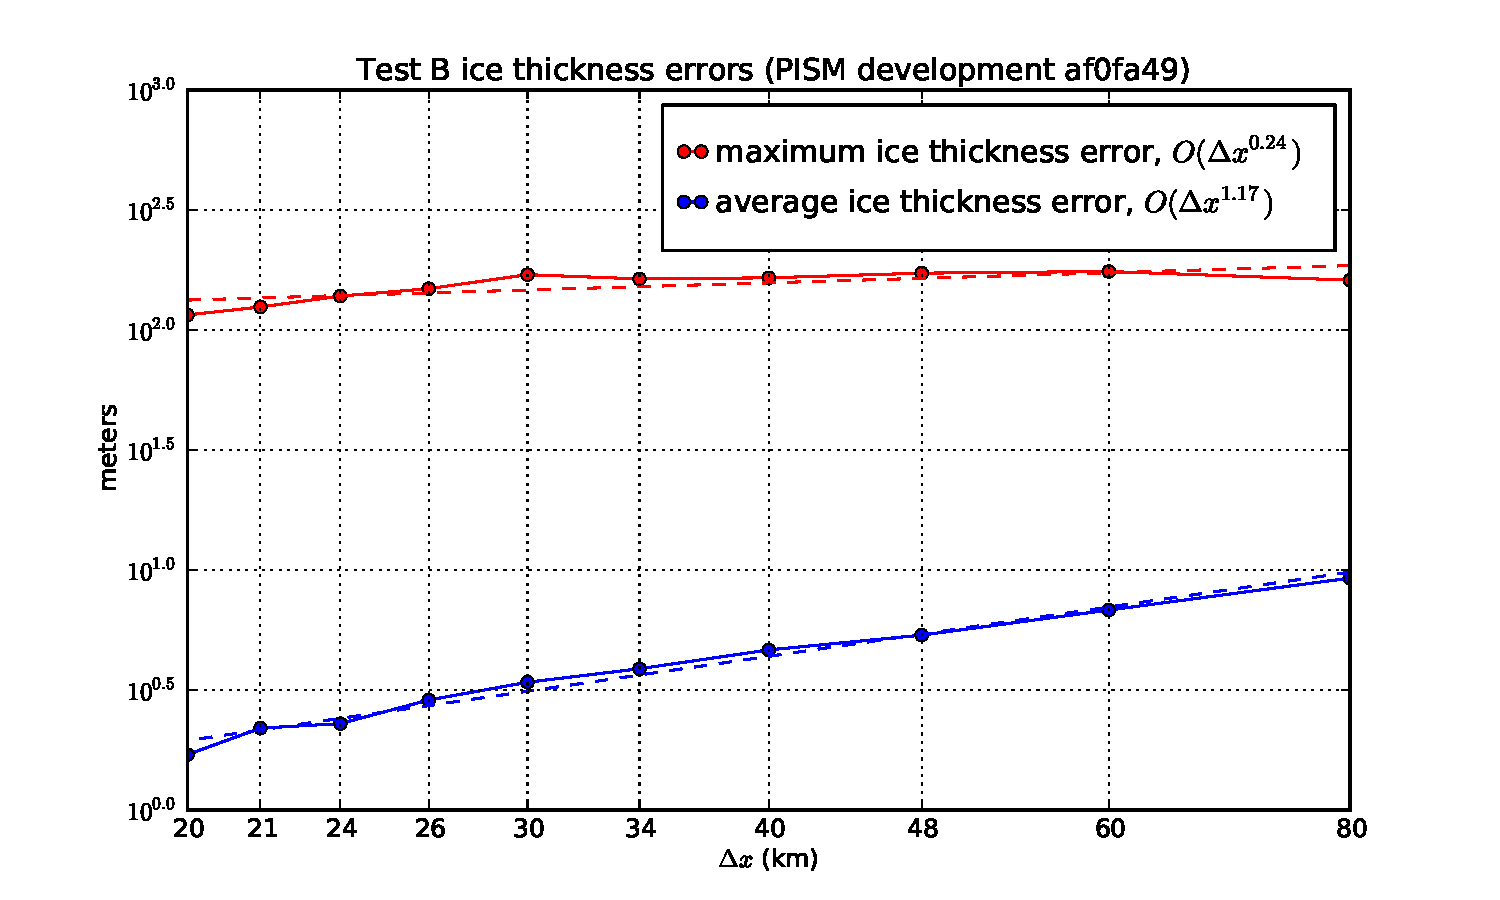
\includegraphics[width=4.8in,keepaspectratio=true]{test-B-thickness}
\caption{Numerical thickness errors in test B. See \cite{BLKCB} for discussion.}
\label{fig:thickerrsB}
\end{figure}

\begin{figure}[ht]
\centering
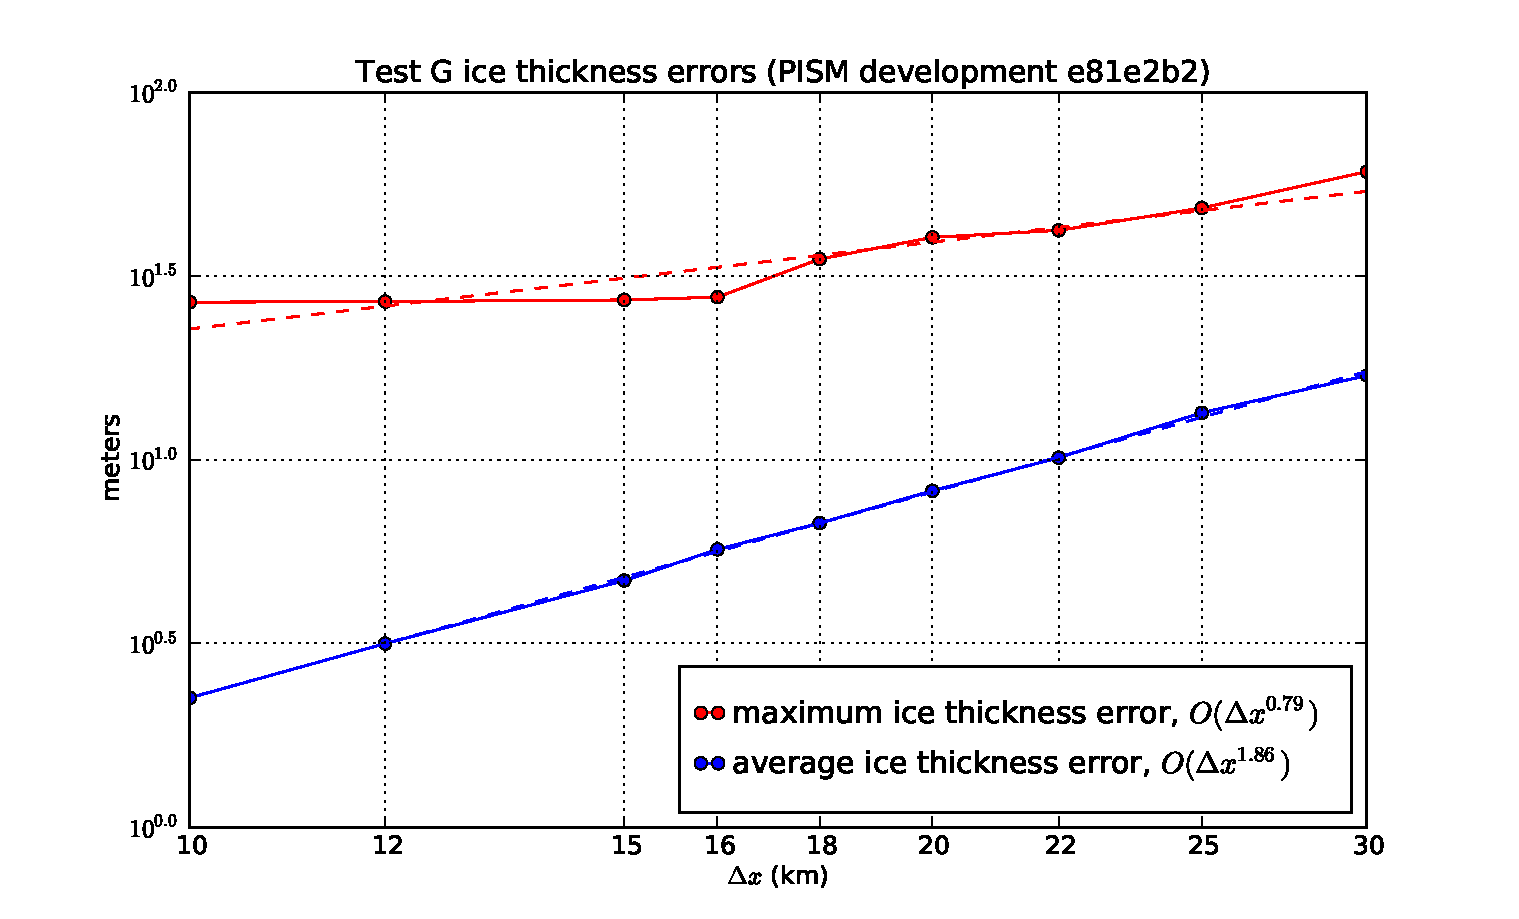
\includegraphics[width=5.0in,keepaspectratio=true]{test-G-thickness}
\caption{Numerical thickness errors in test G.  See \cite{BBL} and \cite{BLKCB}.}
\label{fig:thickerrsG}
\end{figure}

\begin{figure}[ht]
\centering
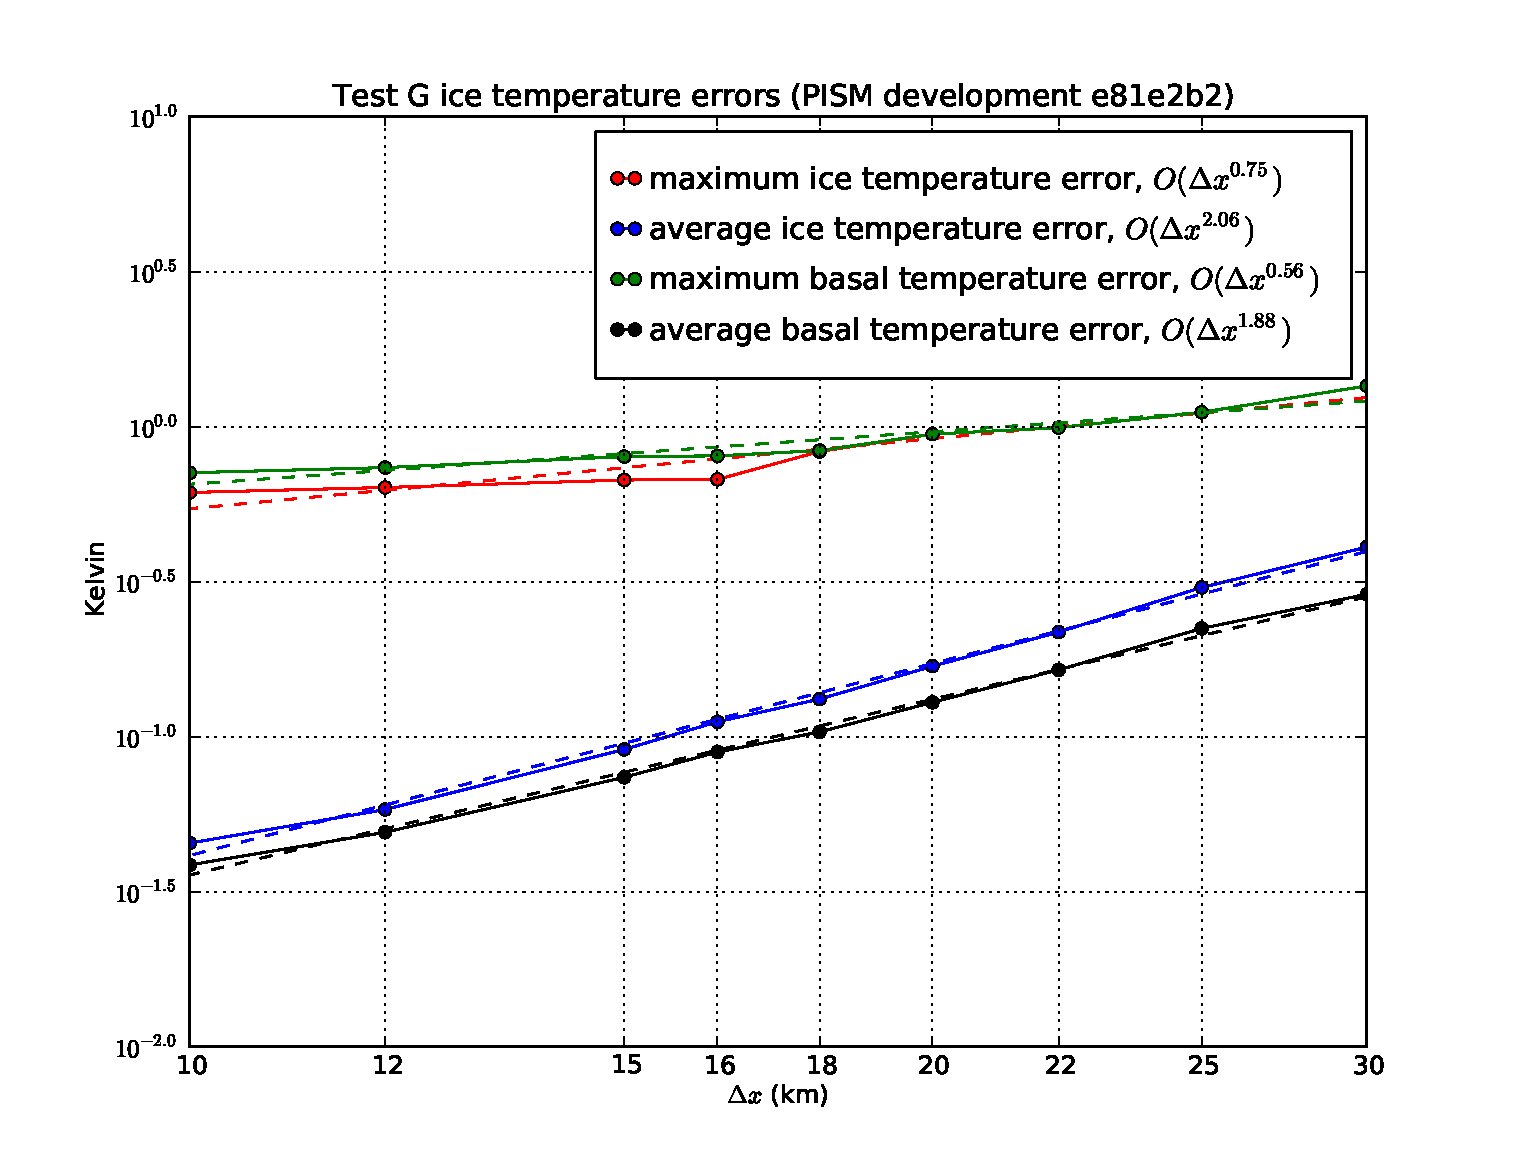
\includegraphics[width=5.0in,keepaspectratio=true]{test-G-temp}
\caption{Numerical temperature errors in test G. See \cite{BBL}.}
\label{fig:temperrsG}
\end{figure}

\begin{figure}[ht]
\centering
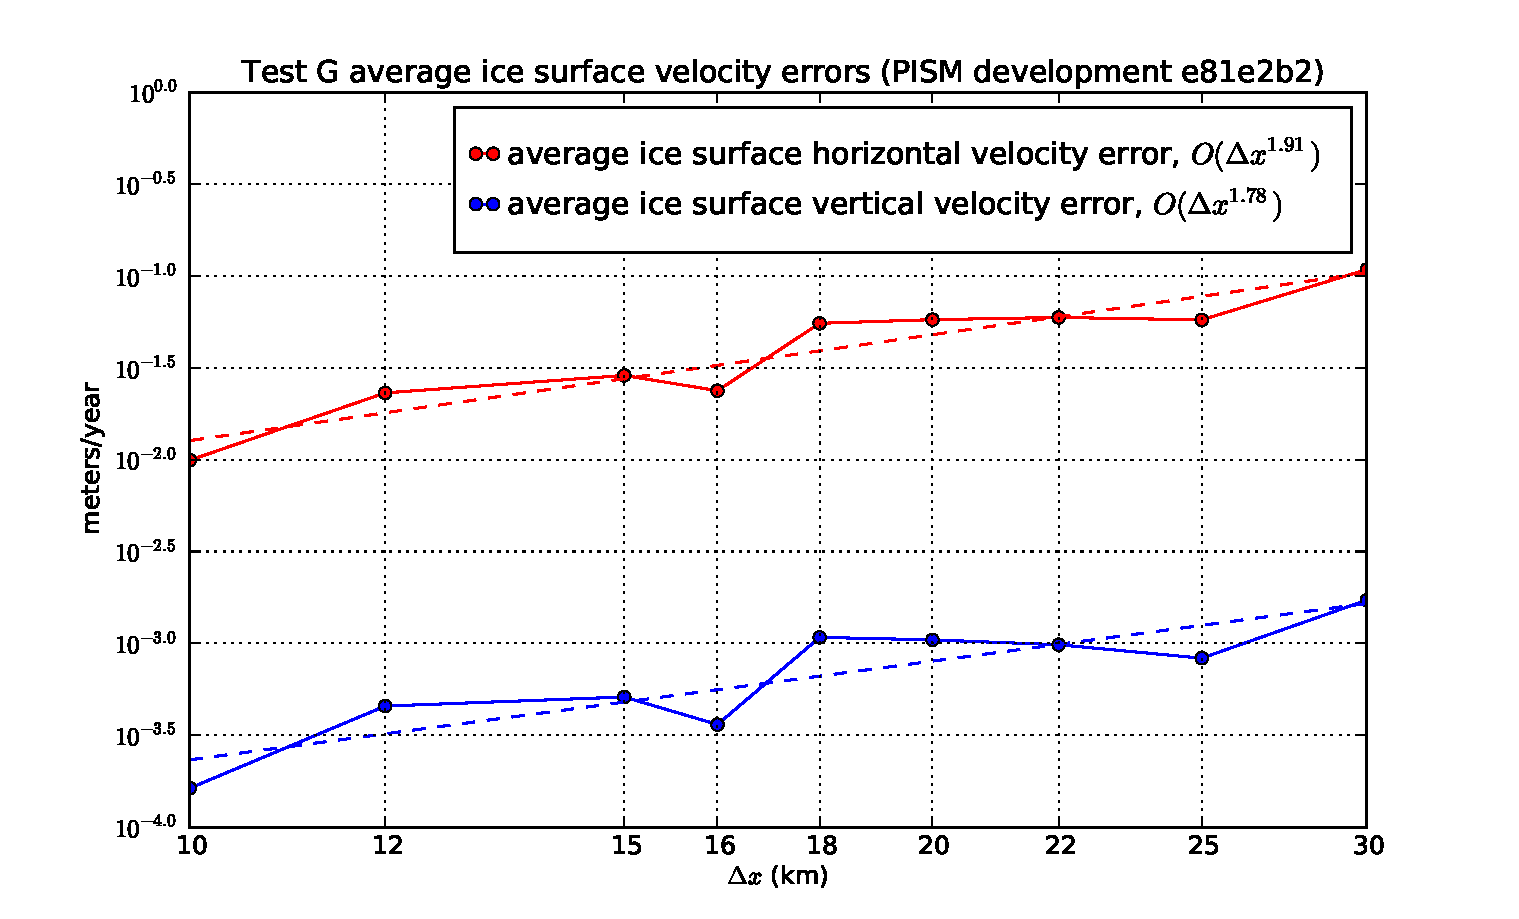
\includegraphics[width=5.0in,keepaspectratio=true]{test-G-surfvels}
\caption{Numerical errors in computed surface velocities in test G.}
\label{fig:surfvelerrsG}
\end{figure}

\begin{figure}[ht]
\centering
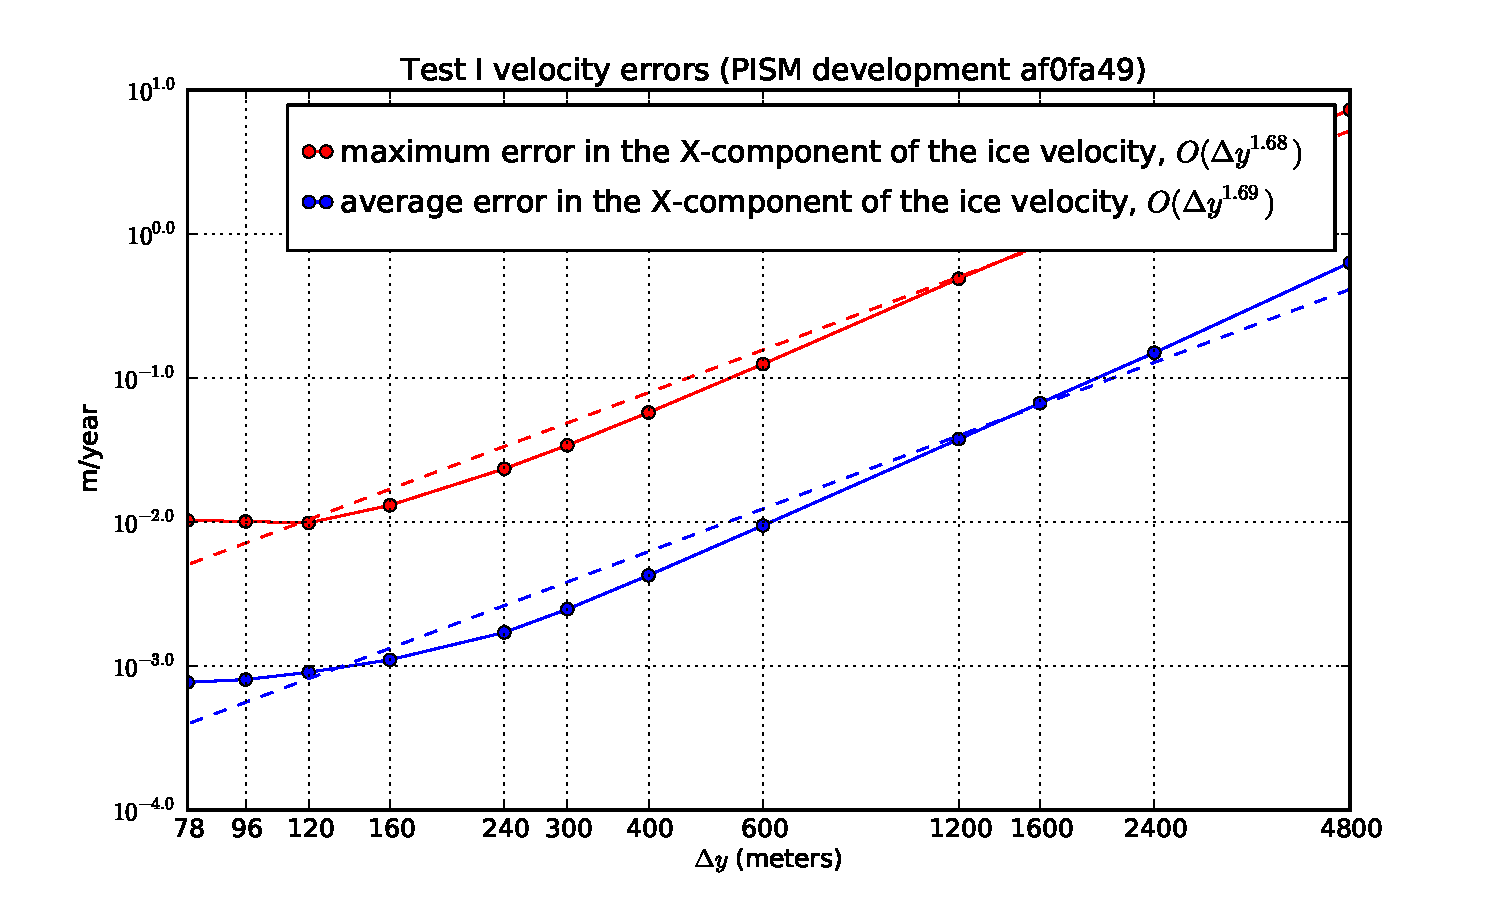
\includegraphics[width=5.0in,keepaspectratio=true]{test-I-errors}
\caption{Numerical errors in horizontal velocities in test I, an ice stream. See \cite{SchoofStream,BBssasliding}.}
\label{fig:velerrsI}
\end{figure}

%%% Local Variables: 
%%% mode: latex
%%% TeX-master: "manual"
%%% End: 


\clearpage\newpage

\section{Simplified geometry experiments with PISM}\label{sec:simp}

\subsubsection*{Historical note}  There have been three stages of ice sheet model intercomparisons based on simplified geometry experiments since the early 1990s \cite{BuelerSpray}.\index{EISMINT!defined}

EISMINT I \cite[ European Ice Sheet Modeling INiTiative]{EISMINT96}\footnote{See \url{http://homepages.vub.ac.be/\%7Ephuybrec/eismint.html}.} was the first of these and involved only the isothermal shallow ice approximation (SIA).  Both fixed margin and moving margin experiments were performed in EISMINT I, and various conclusions were drawn about the several numerical schemes used in the intercomparison.  EISMINT I is superceded, however, by verification using the full variety of known exact solutions to the isothermal SIA \cite{BLKCB}.  The ``rediscovery'', since EISMINT I, of the Halfar similarity solution with zero accumulation \cite{Halfar83}, and verification runs using that solution, already suffices to measure the isothermal SIA performance of PISM more precisely than would be allowed by comparison to EISMINT I results.

EISMINT II \cite{EISMINT00} pointed out interesting and surprising properties of the thermocoupled SIA.  References \cite{BBL,Hindmarsh04,Hindmarsh06,PayneBaldwin,SaitoEISMINT,BBssasliding} each interpret the EISMINT II experiments and/or describe attempts to add more complete physical models to ``fix'' the (perceived and real) shortfalls of ice sheet model behavior on EISMINT II experiments.  We believe that the discussion in \cite{PayneDongelmans,PayneBaldwin,BBL} adequately explains the ``spokes'' in EISMINT II experiment F as a genuine fluid instability, while Appendix B of \cite{BBssasliding} adequately cautions against the continuum model that generates the ``spokes'' in EISMINT II experiment H.   Thus we can move on from that era of controversy.  In any case, PISM has built-in support for all of the published and unpublished EISMINT II experiments; these are described in the next subsection.

The ISMIP (Ice Sheet Model Intercomparison Project)\footnote{See \url{http://homepages.vub.ac.be/\%7Ephuybrec/ismip.html}.}\index{ISMIP!defined} round of intercomparisons is still ongoing at this time (2009).  There are two components of ISMIP substantially completed, namely HOM = Higher Order Models \cite{ISMIPHOM,HOMelmer} and HEINO = Heinrich Event INtercOmparison \cite{GreveTakahamaCalov,Calovetal2009HEINOfinal}.  Of these, PISM participated in HEINO, but this ability is unmaintained.   We believe\index{ISMIP!interpretation of HEINO results} the continuum problem described by HEINO, also used in EISMINT II experiment H (above), is not easily approximate-able because of a required discontinuous jump in the basal velocity field.  The continuum problem predicts infinite vertical velocity because of this jump \cite[Appendix B]{BBssasliding}.  Details of the numerical schemes and their results are irrelevant if the continuum model makes such a prediction.

PISM offers the physical continuum model described in \cite{BBssasliding}, an SIA/SSA hybrid, as an alternative to the continuum model used in ISMIP-HEINO and EISMINT II experiment H.  Indeed the SIA/SSA hybrid is offered as a unified shallow model for real ice sheets (section \ref{sec:dynamics}).

There is no current plan to support ISMIP-HOM, but comparison of shallow PISM results to exact Stokes solutions is a goal for PISM evaluation.

A third ISMIP part is the Marine Ice Sheet Model Intercomparison Project (MISMIP)\index{ISMIP!MISMIP}.  It is minimally supported in PISM, as described in subsection \ref{subsect:MISMIP} below.


\subsection{EISMINT II}\label{subsect:EISMINTII}
\optsection{EISMINT II}

There are seven experiments described in the published EISMINT II writeup \cite{EISMINT00}.\index{EISMINT}  They are named A, B, C, D, F, G, and H.  They have these common features:\begin{itemize}
\item runs are for 200,000 years, with no prescribed time step;
\item a $61\times 61$ horizontal grid on a square domain ($1500$ km side length) is prescribed;
\item the surface inputs (temperature and mass balance) have angular symmetry around the center of the grid;
\item the bed is flat and does not move (no isostasy);
\item the temperature in the bedrock is not modeled;
\item only the cold (not polythermal) thermomechanically-coupled shallow ice approximation is used \cite{EISMINT00}; and
\item though basal melt rates may be computed diagnostically, they do not affect the evolution of the ice sheet.
\end{itemize}
The experiments differ from each other in their various combinations of surface temperature and mass balance parameterizations.  Experiments H and G involve basal sliding, under the physically-dubious SIA sliding rubric \cite[Appendix B]{BBssasliding}, while the others don't.  Four experiments start with zero ice (A,F,G,H), while the other experiments (B,C,D) start from the final state of experiment A.

In addition to the seven experiments published in \cite{EISMINT00}, there were an additional five experiments described in the EISMINT II intercomparison description 
\cite{EISIIdescribe}, labeled E, I, J, K, and L.\index{EISMINT!unpublished additional EISMINT II experiments}  These experiments share most features listed above, but with the following differences.  Experiment E is the same as experiment A except that the peak of the accumulation, and also the low point of the surface temperature, are shifted by 100 km in both $x$ and $y$ directions; also experiment E starts with the final state of experiment A.  Experiments I and J are similar to experiment A but with non-flat ``trough'' bed topography.  Experiments K and L are similar to experiment C but with non-flat ``mound'' bed topography.

See table \ref{tab:eisII} for how to run all EISMINT II experiments in PISM.  Note that the vertical grid is not specified in EISMINT II, and it seems that good simulation of the thermomechanically-coupled conditions near the base of the ice requires relatively-fine resolution there.  (It is difficult to be quantitative because of a lack of theory.)  We suggest using the default unequally-spaced grid with 61 levels, which gives a grid spacing of 21 m in the ice layer closest to the bed.\footnote{An equally-spaced grid is an option in PISM, and in this case we suggest using 201 vertical levels to give 25 m spacing.}

These SIA-only simulations parallelize particularly well.  Very roughly, for the standard $61\times 61$ horizontal grid, wall-clock-time speedups will occur up to about 30 processors, and finer grids will benefit from even more processors, of course.

Table \ref{tab:eisII} shows how all EISMINT II experiments are done in PISM.  Experiments below the horizontal line in Table \ref{tab:eisII} are only documented in \cite{EISIIdescribe}.

\begin{table}[ht]
\centering
\small
\begin{tabular}{@{}llll}\toprule
\textbf{Command: ``\texttt{pisms }'' $+$} & \textbf{Relation to experiment A} \\
\midrule
\texttt{-eisII A -Mx 61 -My 61 -Mz 61 -y 200000 -o eisIIA.nc} & \\
\texttt{-eisII B -i eisIIA.nc -y 2e5 -o eisIIB.nc} & warmer \\
\texttt{-eisII C -i eisIIA.nc -y 2e5 -o eisIIC.nc} & less snow (lower accumulation)\\
\texttt{-eisII D -i eisIIA.nc -y 2e5 -o eisIID.nc} & smaller area of accumulation \\
\texttt{-eisII F -Mx 61 -My 61 -Mz 61 -y 2e5 -o eisIIF.nc} & colder; famous spokes \cite{BBL} \\
\texttt{-eisII G -Mx 61 -My 61 -Mz 201 -y 2e5 -o eisIIG.nc} & sliding (regardless of temperature) \\
\texttt{-eisII H -Mx 61 -My 61 -Mz 201 -y 2e5 -o eisIIH.nc} & melt-temperature activated sliding \\ \midrule
\texttt{-eisII E -i eisIIA.nc -y 2e5 -o eisIIE.nc} & shifted climate maps \\
\texttt{-eisII I -Mx 61 -My 61 -Mz 201 -y 2e5 -o eisIII.nc} & trough topography \\
\texttt{-eisII J -i eisIII.nc -y 2e5 -o eisIIJ.nc} & trough topography and less snow \\
\texttt{-eisII K -Mx 61 -My 61 -Mz 201 -y 2e5 -o eisIIK.nc} & mound topography \\
\texttt{-eisII L -i eisIIK.nc -y 2e5 -o eisIIL.nc} & mound topography and less snow \\
\bottomrule
\normalsize
\end{tabular}
\label{tab:eisII}
\caption{Running the EISMINT II experiments in PISM.\index{PISM!running the EISMINT II experiments in}  Use \texttt{-skip -skip_max 5}, on the $61\times 61$ default grid, for significant speedup.}
\end{table}

The EISMINT II experiments can be run with various modifications of the default settings.  Of course the grid can be refined.  For instance, a twice as fine grid in the horizontal is ``\texttt{-Mx 121 -My 121}''.  Table \ref{tab:eisIIoptions} lists some optional settings which are particular to the EISMINT II experiments.

\begin{table}[ht]
\centering
\small
\begin{tabular}{@{}lp{0.35\linewidth}lp{0.35\linewidth}}\toprule
\textbf{Option} & \textbf{Default values [expers]} & \textbf{Units} & \textbf{Meaning} \\\midrule
\intextoption{eisII} & A & &  Choose single character name of EISMINT II \cite{EISMINT00} simplified geometry experiment.  Allowed values are A, B, C, D, E, F, G, H. \\
\intextoption{Mmax} & 0.5 [ABDEFGHIK], 0.25 [CJL] & m$/$a & max value of accumulation rate \\
\intextoption{Rel} & 450 [ABEFGHIK], 425 [CDJL] & km & radial distance to equilibrium line \\
\intextoption{Sb} & $10^{-2}$ [\emph{all}] & (m/a)/km & radial gradient of accumulation rate \\
\intextoption{ST} & $1.67 \times 10^{-2}$ [\emph{all}] & K/km & radial gradient of surface temperature\\
\intextoption{Tmin} & 238.15 [ACDEGHIJKL], & K & max of surface temperature \\
 & 243.15[B], 223.15[F] & & \\
\intextoption{bmr_in_cont} & & & Include the basal melt rate in the mass continuity computation (override default for EISMINT II)\\
\bottomrule\normalsize
\end{tabular}
\label{tab:eisIIoptions}
\caption{Changing the default settings for EISMINT II}
\end{table}

In PISM the height of the computational box, the quantity set by \texttt{-Lz}, is set at the beginning of the run.  It is chosen for the EISMINT II experiments according to the observed maximum values occuring in standard runs.  If the ice thickens beyond the chosen level for the top of the computational box then additional layers are automatically added to the computational grid.  In fact, if the ice grows above the height of the computational box then a message appears, \texttt{PISM WARNING: max ice thickness ... is greater than the height of the computational box ...}, and then at least two additional levels are added to the vertical grid.  This is to some degree an emergency mechanism, however, because it can run away to use up all memory in extreme cases.  If the height of the computational box grows so large that the grid has more than twice the original number of vertical levels then PISM produces a \texttt{PISM ERROR} error message and stops.   Therefore it is possible that the number of vertical levels at the end of the run exceeds the initial \texttt{-Mz} value.  Setting EISMINT II options \texttt{-Mmax} or \texttt{-Sb} to produce higher accumulation rates than the default values (see table \ref{tab:eisIIoptions}) may cause the ice sheet to thicken above the standard thickness and therefore trigger this automatic extension mechanism.  Similarly, colder ice caused by nonstandard \texttt{-Tmin} or \texttt{-ST} values can produce unusually thick ice.  The user may always choose to use a larger, more conservative value for option \texttt{-Lz}, however.


\subsection{MISMIP}\label{subsect:MISMIP}
\optsection{MISMIP}

This intercomparison addresses grounding line dynamics by considering an idealized one-dimensional stream-shelf system.  The intercomparison process is described at the website

\centerline{\url{http://homepages.ulb.ac.be/~fpattyn/mismip/}}

\noindent Find a full text description there.  It is essential reading for understanding MISMIP results generally, and for appreciating many of the comments in this subsection.

PISM's version of MISMIP includes an attached ice shelf even though modeling the shelf is theoretically unnecessary in the MISMIP flow line case.  The analysis in \cite{SchoofMarine1} shows that the only effect of an ice shelf, in the flow line case, is to transfer the force imbalance at the calving front directly to the ice column at the grounding line.  But this analysis does not apply to ice shelves with two horizontal dimensions, of course.  Real ice shelves have ``buttressing'' and ``side drag'' and other forces not present in flow line circumstances \cite{Goldbergetal2009}.  See the Ross ice shelf example in section \ref{sec:ross}, for example.

We use the usual PISM ice shelf model, with two horizontal dimensions, to do MISMIP.  This intercomparison therefore looks at the grounding line dynamics results from the usual PISM code, though in a highly symmetric case without side drag.

Because PISM is a model with two horizontal dimensions, we must adapt it to do a flow line problem (see section \ref{sec:flowline-modeling}). The flow direction for MISMIP is arbitrarily taken to be ``$x$''.  We periodize the cross-flow direction ``$y$'', and use the minimum number of points in this direction which maintains function.  This number turns out to be ``\texttt{-My 3}''; fewer points than this in the cross-flow direction confuses the finite difference scheme.

PISM has two applicable ice dynamics models. Model 1 is a pure SSA model.  It is ``category 2'' in the MISMIP classification.  Model 2 combines SIA and SSA velocities as described in \cite{BBssasliding}, and is ``category 3'' because it resolves ``vertical'' shear (i.e.~using SIA flow).

There are many runs for a complete MISMIP intercomparison submission.  There are $62$ runs for each model and grid choice, and there are two models and three (suggested) grid choices, so a full suite is $6 \times 62 = 372$ runs.  The finest grid runs account for all the compute time, however.  ``Grid mode 2'' in the MISMIP description is 1500 grid spaces in the flow line direction\footnote{This translates into 3001 grid \emph{points} in PISM's doubled computational domain.}, a very fine grid which imposes severe time-step restrictions on the explicit methods in PISM.  For the PISM MISMIP submission in Sept.~2008 we chose to only submit runs for a grid with 150 (``grid mode 1'') and 600 (``grid mode 3'') grid spaces in the flow line direction.  This was still 248 runs to submit, with 3 files each for a total of 744 text files.

Please see \texttt{README.md} in \texttt{examples/mismip} for a description of the setup that can be used to run MISMIP experiments in PISM.

\begin{figure}[ht]
\centering
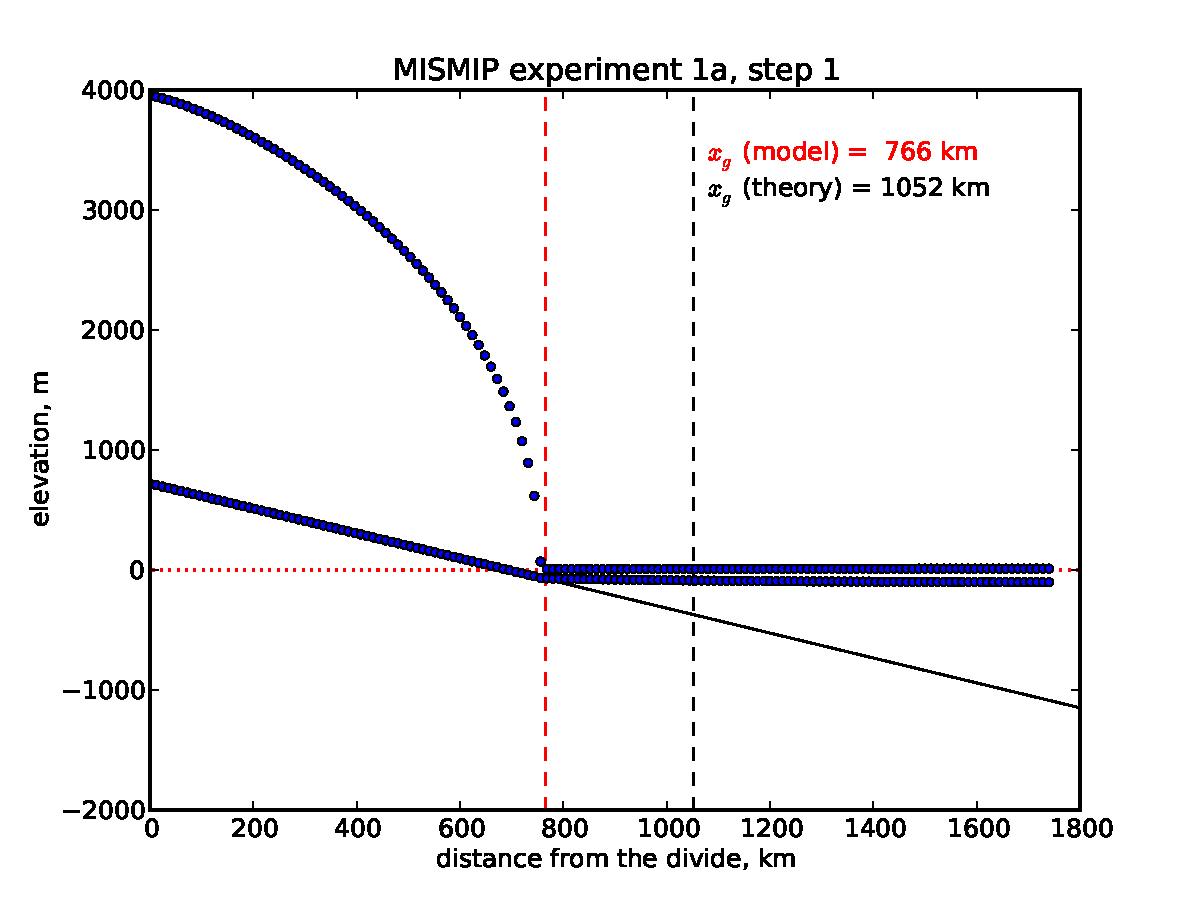
\includegraphics[width=4.0in,keepaspectratio=true]{CKH1-1a-M1-A1-profile}
\caption{A marine ice sheet profile in the MISMIP intercomparison; PISM model 1, experiment 1a, grid mode 1, step 1. Starting from a uniform $10$ m ice thickness.}
\label{fig:MISMIPmodel1exper1aM1A1}
\end{figure}

The implementation of MISMIP in PISM conforms fairly closely to the intercomparison description.  However, that document specifies
\begin{quotation}
\dots we require that the rate of change of grounding line position be $0.1$ m/a or less, while the rate of change of ice thickness at each grid point at which ice thickness is defined must be less than $10^{-4}$ m/a \dots
\end{quotation}
as a standard for ``steady state''. PISM does not include a stopping criterion such as ones described here. However, we report enough information, in PISM output files with scalar and spatially-variable time-series, to compute a grounding line rate or the time at which the thickness rate of change drops below $10^{-4}$ m/a.

One of the physical parameters regarding PISM's ice shelf model needs comment: we make the base of the ice shelves have very small resistance, using $10^{-4}$ times the linear drag typical of a Siple coast ice stream \cite{HulbeMacAyeal}, because this seems to have the effect of stabilizing the ice shelf.

\begin{figure}[ht]
\centering
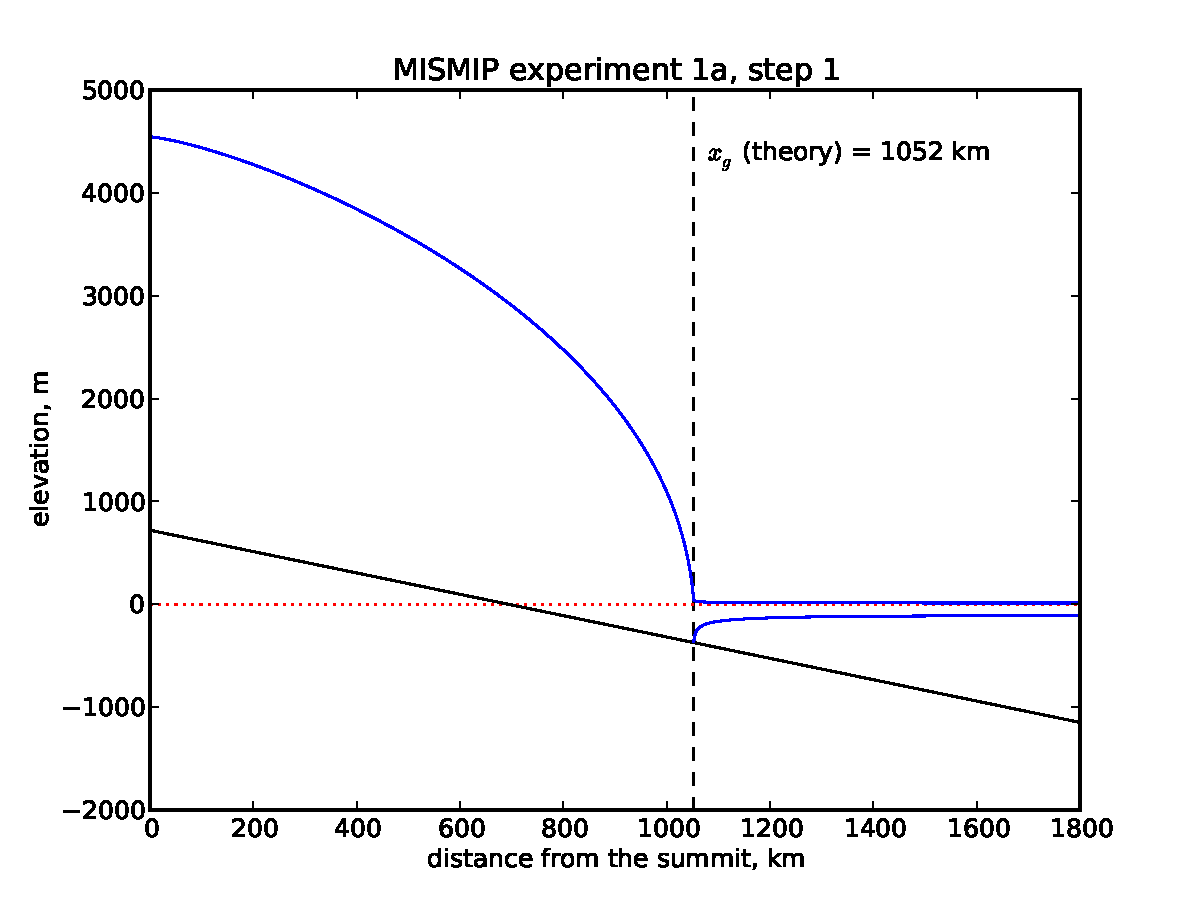
\includegraphics[width=4.0in,keepaspectratio=true]{SM-1a-A1}
\caption{Analytical profile for steady state of experiment 1a, grid mode 1, step 1, from theory in \cite{SchoofMarine1}.  This is a boundary layer asymptotic matching result, but not the exact solution to the equations solved numerically by PISM. Compare Figures \ref{fig:MISMIPmodel1exper1aM1A1} and \ref{fig:MISMIPmodel1exper1aM3A1FROMSM} generated by PISM.}
\label{fig:SMexper1aM1A1}
\end{figure}

The script \texttt{MISMIP.py} in \texttt{examples/mismip} has the ability to compute the profile from the Schoof's \cite{SchoofMarine1} asymptotic-matching boundary layer theory.  This script is a Python translation, using \texttt{scipy} and \texttt{pylab}, of the \Matlab codes in \url{http://homepages.ulb.ac.be/~fpattyn/mismip/MISMIP_distribution.tar}.  For example,

\begin{verbatim}
$ python MISMIP.py
\end{verbatim}

\noindent produces Figure \ref{fig:SMexper1aM1A1}.

We see immediately that the PISM result does not put the grounding line in the same location as Schoof's boundary layer theory.  We believe the problem is with PISM's numerical solution, not with that theory.  More evidence that the problem is numerical can be found by looking at the ice flux.  Using \texttt{ncview} to examine the diagnostic variable \texttt{cflx} (magnitude) in \texttt{ABC1_1a_M1_A1.nc} we see Figure \ref{fig:cflx1aM1A1}.  \emph{This is a problem with PISM}.  The flux should be a linear function.  Indeed, at steady state the flux $\bq$ solves $a=\Div\bq$ where $a$ is the accumulation rate.  In MISMIP, $a$ is the constant $0.3$ m/a, so at steady state $|\bq| = a x$, a line.

\begin{figure}[ht]
\centering
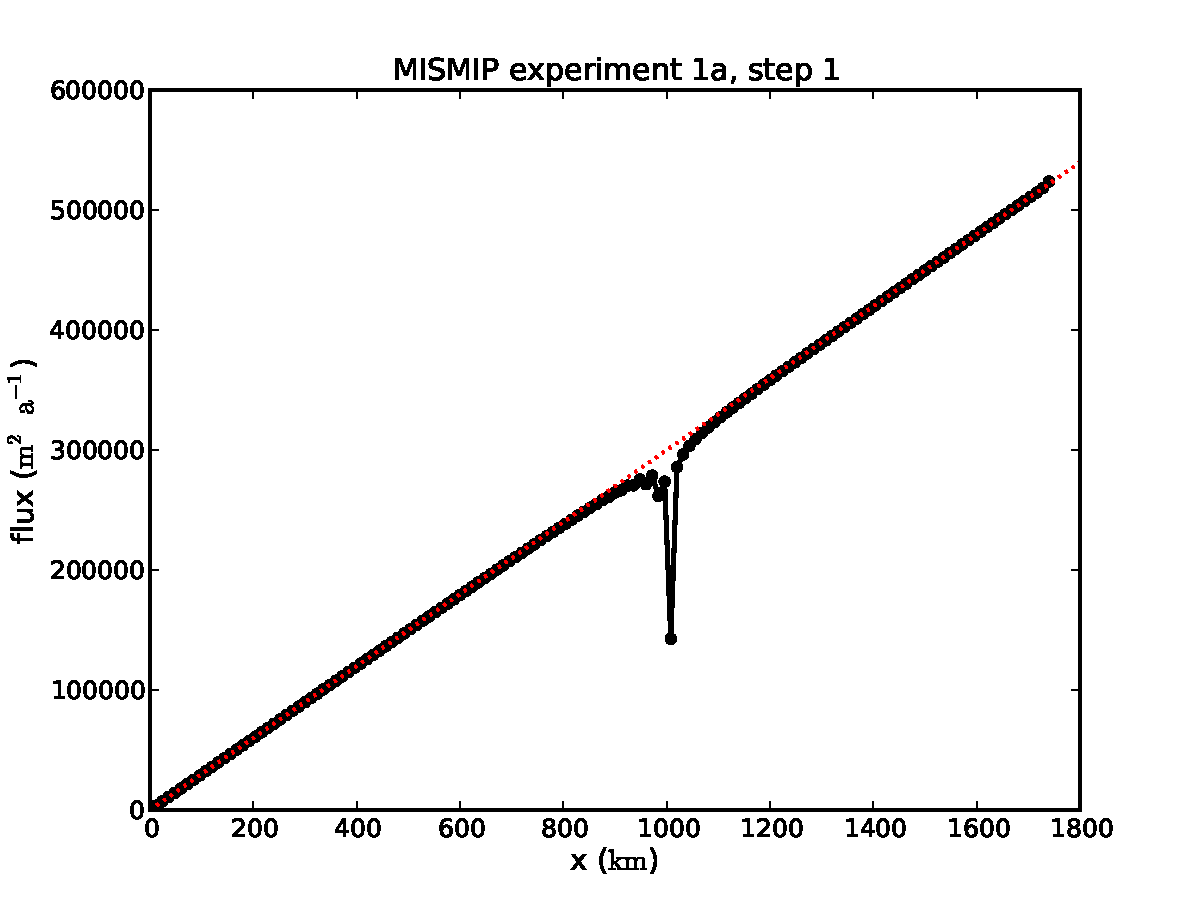
\includegraphics[width=4.0in,keepaspectratio=true]{CKH1-1a-M1-A1-flux}
\caption{Numerically computed flux $\bq = \bar\bU\, H$, where $\bar\bU$ is the vertically-averaged horizontal velocity and $H$ the thickness, for steady state of experiment 1a, grid mode 1, step 1.  Illustrates a significant numerical problem; it should be the dotted line, which has slope $a = 0.3$ m/a.}
\label{fig:cflx1aM1A1}
\end{figure}

We can learn more about the problem.  It turns out that the numerical flaw in the flux also keeps the grounding line from moving properly, we think.  The problem is that the numerical result doesn't move the grounding line to its correct location if the ice sheet and shelf are initially $10$ m as specified in MISMIP.  On the other hand, the correct location for the grounding line is also approximately a steady state for PISM numerics; the grounding line stays where you put it (compare \cite{SchoofMarine2} and \cite{VieliPayne}).

In fact, by default \texttt{run.py} uses the asymptotic-matching thickness result from the \cite{SchoofMarine1} theory to initialize the initial ice thickness, as allowed by the MISMIP specification.

The effect when we do this at higher resolution (grid mode 3 with 6km spacing, instead of 24 km), is a step forward.
The result, Figure \ref{fig:MISMIPmodel1exper1aM3A1FROMSM}, is more satisfactory.  On the other hand, inspection of the flux for this new run shows a smaller, but similarly worrying, jump in flux.

\begin{figure}[ht]
\centering
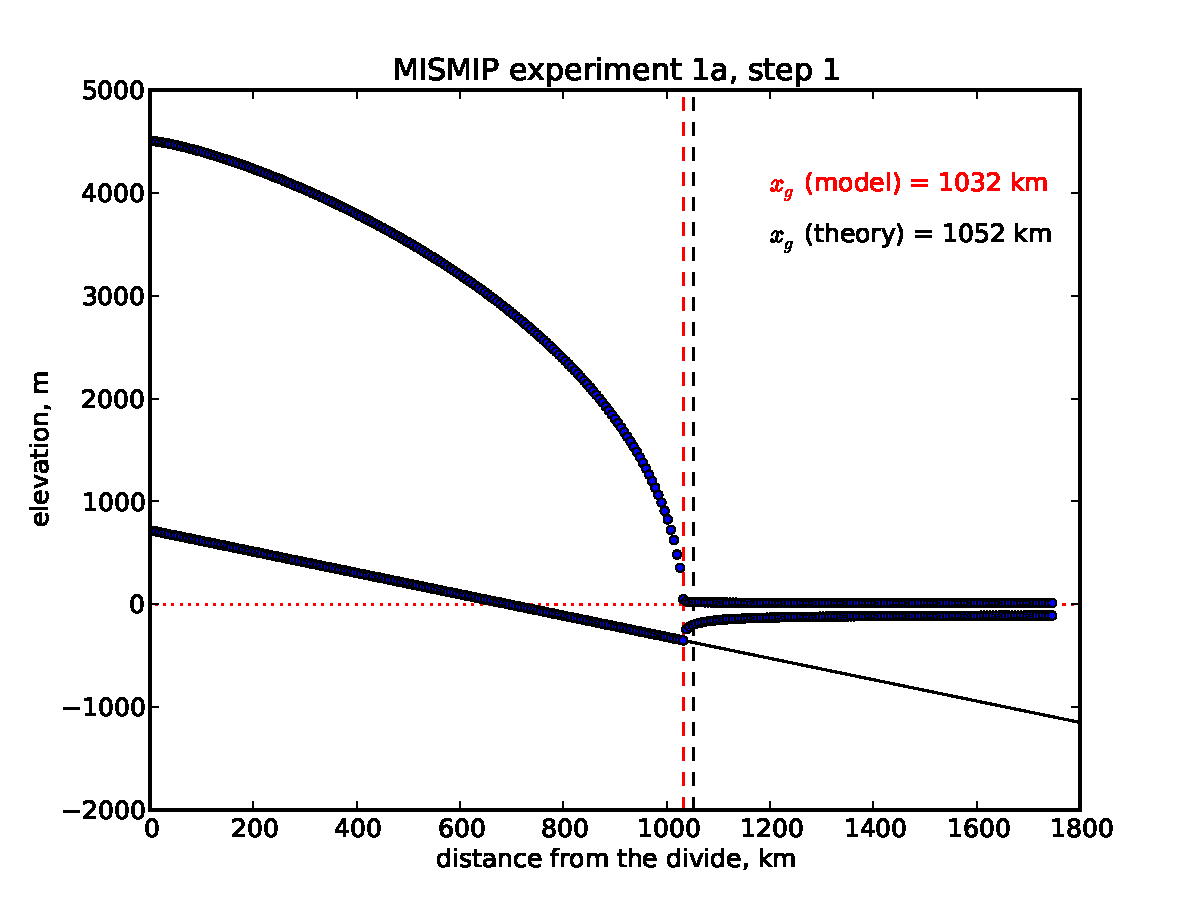
\includegraphics[width=4.0in,keepaspectratio=true]{CKH1-1a-M3-A1-profile}
\caption{A marine ice sheet profile in the MISMIP intercomparison; PISM model 1, experiment 1a, grid mode 3, step 1, but on a run started from the corresponding asymptotic-matching result.  At least the location of the grounding line agrees more closely with that in Figure \ref{fig:SMexper1aM1A1}.}
\label{fig:MISMIPmodel1exper1aM3A1FROMSM}
\end{figure}


%%% Local Variables: 
%%% mode: latex
%%% TeX-master: "manual"
%%% End: 


\clearpage\newpage

\section{Example: Validating PISM as a flow model for the Ross ice shelf}\label{sec:ross} \index{PISM! diagnostic Ross ice shelf setup}\index{Ice Sheets!Antarctic ice sheet!Ross ice shelf} \index{PISM!validation of ice shelf model} \index{Ross ice shelf}
\optsection{Ross}

The term ``validation'' describes the comparison of model output with physical observations in cases where those physical observations are believed to be sufficiently complete and of sufficient quality so that the performance of the numerical model can be assessed \cite{Roache,Wesseling}.  Roughly speaking, validation can happen when the observations or data are better than the model, so the comparison measures the quality of the numerical model and not merely errors in, incompleteness of, or lack of confidence in, the data.

As part of the first EISMINT series of intercomparisons, MacAyeal and others \cite{MacAyealetal} validated several ice shelf numerical models using the Ross ice shelf as an example.  We refer to this intercomparison and its associate write-up \cite{MacAyealetal} as ``EISMINT-Ross''.  The models were compared to data from RIGGS (the Ross Ice shelf Geophysical and Glaciological Survey \cite{RIGGS2,RIGGS1}), acquired in the period 1973--1978.   The RIGGS data include the (horizontal) velocity of the ice shelf measured at a few hundred locations in a reasonably regular grid across the shelf.

Substantial developments have occurred in the modeling of the Ross ice shelf since the EISMINT-Ross intercomparison.  For example, inverse modeling techniques were used to recover depth-averaged viscosity of the Ross ice shelf from the RIGGS data in \cite{RommelaereMacAyeal}. A parameter-sensitivity study was performed for a particular Ross ice shelf numerical model in \cite{HumbertGreveHutter}.

Previous PISM versions included a specialized executable \texttt{pross} that set up the EISMINT-Ross flow model and performed the diagnostic computation.

Increased availability of data sets for ice sheet modeling (see \cite{LeBrocqetal2010} and \cite{Rignot09092011} in particular) make it possible to create a similar setup using modern, higher-quality, higher-resolution data.

The scripts in this section are found in the directory \texttt{examples/ross/}.  The script \texttt{preprocess.py} will download data and build a NetCDF input file. Then \texttt{run.sh} can run \texttt{pismr} as described below.

\subsubsection*{Grabbing the data}

Our setup uses geometry and surface boundary condition data from the ALBMAP v1 dataset \cite{LeBrocqetal2010} and MEaSUREs InSAR-Based Antarctica Velocity Map \cite{Rignot09092011} for velocity boundary conditions, both publicly available.\footnote{Please see \texttt{preprocess.py} for URLs.}

We use NetCDF Operators to cut out the relevant portion of the grid and CDO to interpolate high-resolution (500 m) velocity data onto the coarser (5 km) geometry grid used in ALBMAP.

The NetCDF file \texttt{Ross_combined.nc} produced by \texttt{preprocess.py} contains ice thickness, bed elevations, surface temperature, net accumulation, as well as latitude and longitude values.  All of these are typical of ice sheet modeling data, both in evolution and diagnostic runs.  The file also has variables \texttt{u_ssa_bc} and \texttt{v_ssa_bc}.  These give the boundary values which are needed for the diagnostic computation of velocity. They are used at all grounded locations and ice shelf cells that are immediate neighbors of grounded ice.
The variable \texttt{bcflag} specifies these location.

Unlike in EISMINT-Ross setup, the data-set with velocity boundary conditions contains measurements in the interior of the shelf. Thanks to this we don't need to look elsewhere for observations we need to validate our model.

\subsubsection*{Diagnostic computation of ice shelf velocity}
A basic Ross ice shelf velocity computation from these data is:

\begin{verbatim}
$ mpiexec -n 4 pismr -boot_file Ross_combined.nc \
          -Mx 211 -My 211 -Mz 21 -Lz 3000 -z_spacing equal \
          -no_sia -no_energy -ssa_floating_only -pik \
          -ssa_dirichlet_bc -y 0 -o out_211.nc -o_order zyx
\end{verbatim}%$
Here we initialize from \texttt{Ross_combined.nc}. The computational grid specified here is the $5$ km data grid used in the ALBMAP.  The maximum thickness of the ice is $2766$ m so we choose a height for the computational box (\texttt{-Lz}) large enough to contain the ice.

Several command-line options require explanation:
\begin{itemize}
\item \texttt{-no_sia} turns off the SIA stress balance computation, since our
  goal is to model the ice shelf. It also side-steps a technical issue: PISM
  uses periodic boundary conditions at domain boundaries and most fields in
  this setup are not periodic. Turning off SIA avoids operations such as
  differencing surface elevation across the domain edges.
\item \texttt{-ssa_dirichlet_bc} reads fields \texttt{u_ssa_bc}, \texttt{v_ssa_bc}, \texttt{bcflag}, and \texttt{thk} from an input file and uses them to prescribe Dirichlet boundary conditions for the SSA velocity (\texttt{u_ssa_bc} and \texttt{v_ssa_bc} are components of the SSA B.C., \texttt{bcflag} is $1$ at B.C. locations and $0$ elsewhere) and \texttt{thk} at $\mathtt{bcflag} = 1$ locations is used as the Dirichlet B.C. condition for the ice thickness. The latter (together with Dirichlet B.C. for the SSA velocity) can be thought of as prescribing ``SSA ice flux'' at given locations in an \emph{evolution} run.
\item \texttt{-ssa_floating_only} uses the SSA stress balance model for the floating ice \emph{only}. In this setup it is equivalent to \texttt{-ssa_sliding}, because SSA velocities at grounded locations are prescribed.
\item \texttt{-pik} enables PIK improvements (see section \ref{sec:pism-pik}). The most important one here is the calving front stress boundary condition (CFBC).
\item \texttt{-y 0} makes PISM stop after the first one-model-second-long ``preliminary'' time-step. The model state is reset after this time-step, making it equivalent to a ``diagnostic'' run.
\end{itemize}

The script \texttt{run.sh} extends the run above by allowing changing grid resolution and using the SSA flow law enhancement factor as a tuning parameter. (There are many reasonable choices of tuning parameters; this is just one of them. One could also use ice softness (in an isothermal setup) or temperature, for example.)

\subsubsection*{Comparison to older EISMINT-Ross results}

The script \texttt{plot.py} used PISM output such as \texttt{out_211.nc} to produce Figure \ref{fig:rosspython}. This run used the enhancement factor of $0.6$. The thin black line outlines the shelf (which is the actual ``modeling domain'' here). Compare to Figure \ref{fig:eisrosspython}, which shows PISM results using the EISMINT-Ross setup circa 2011.

\begin{figure}[ht]
\centering
\mbox{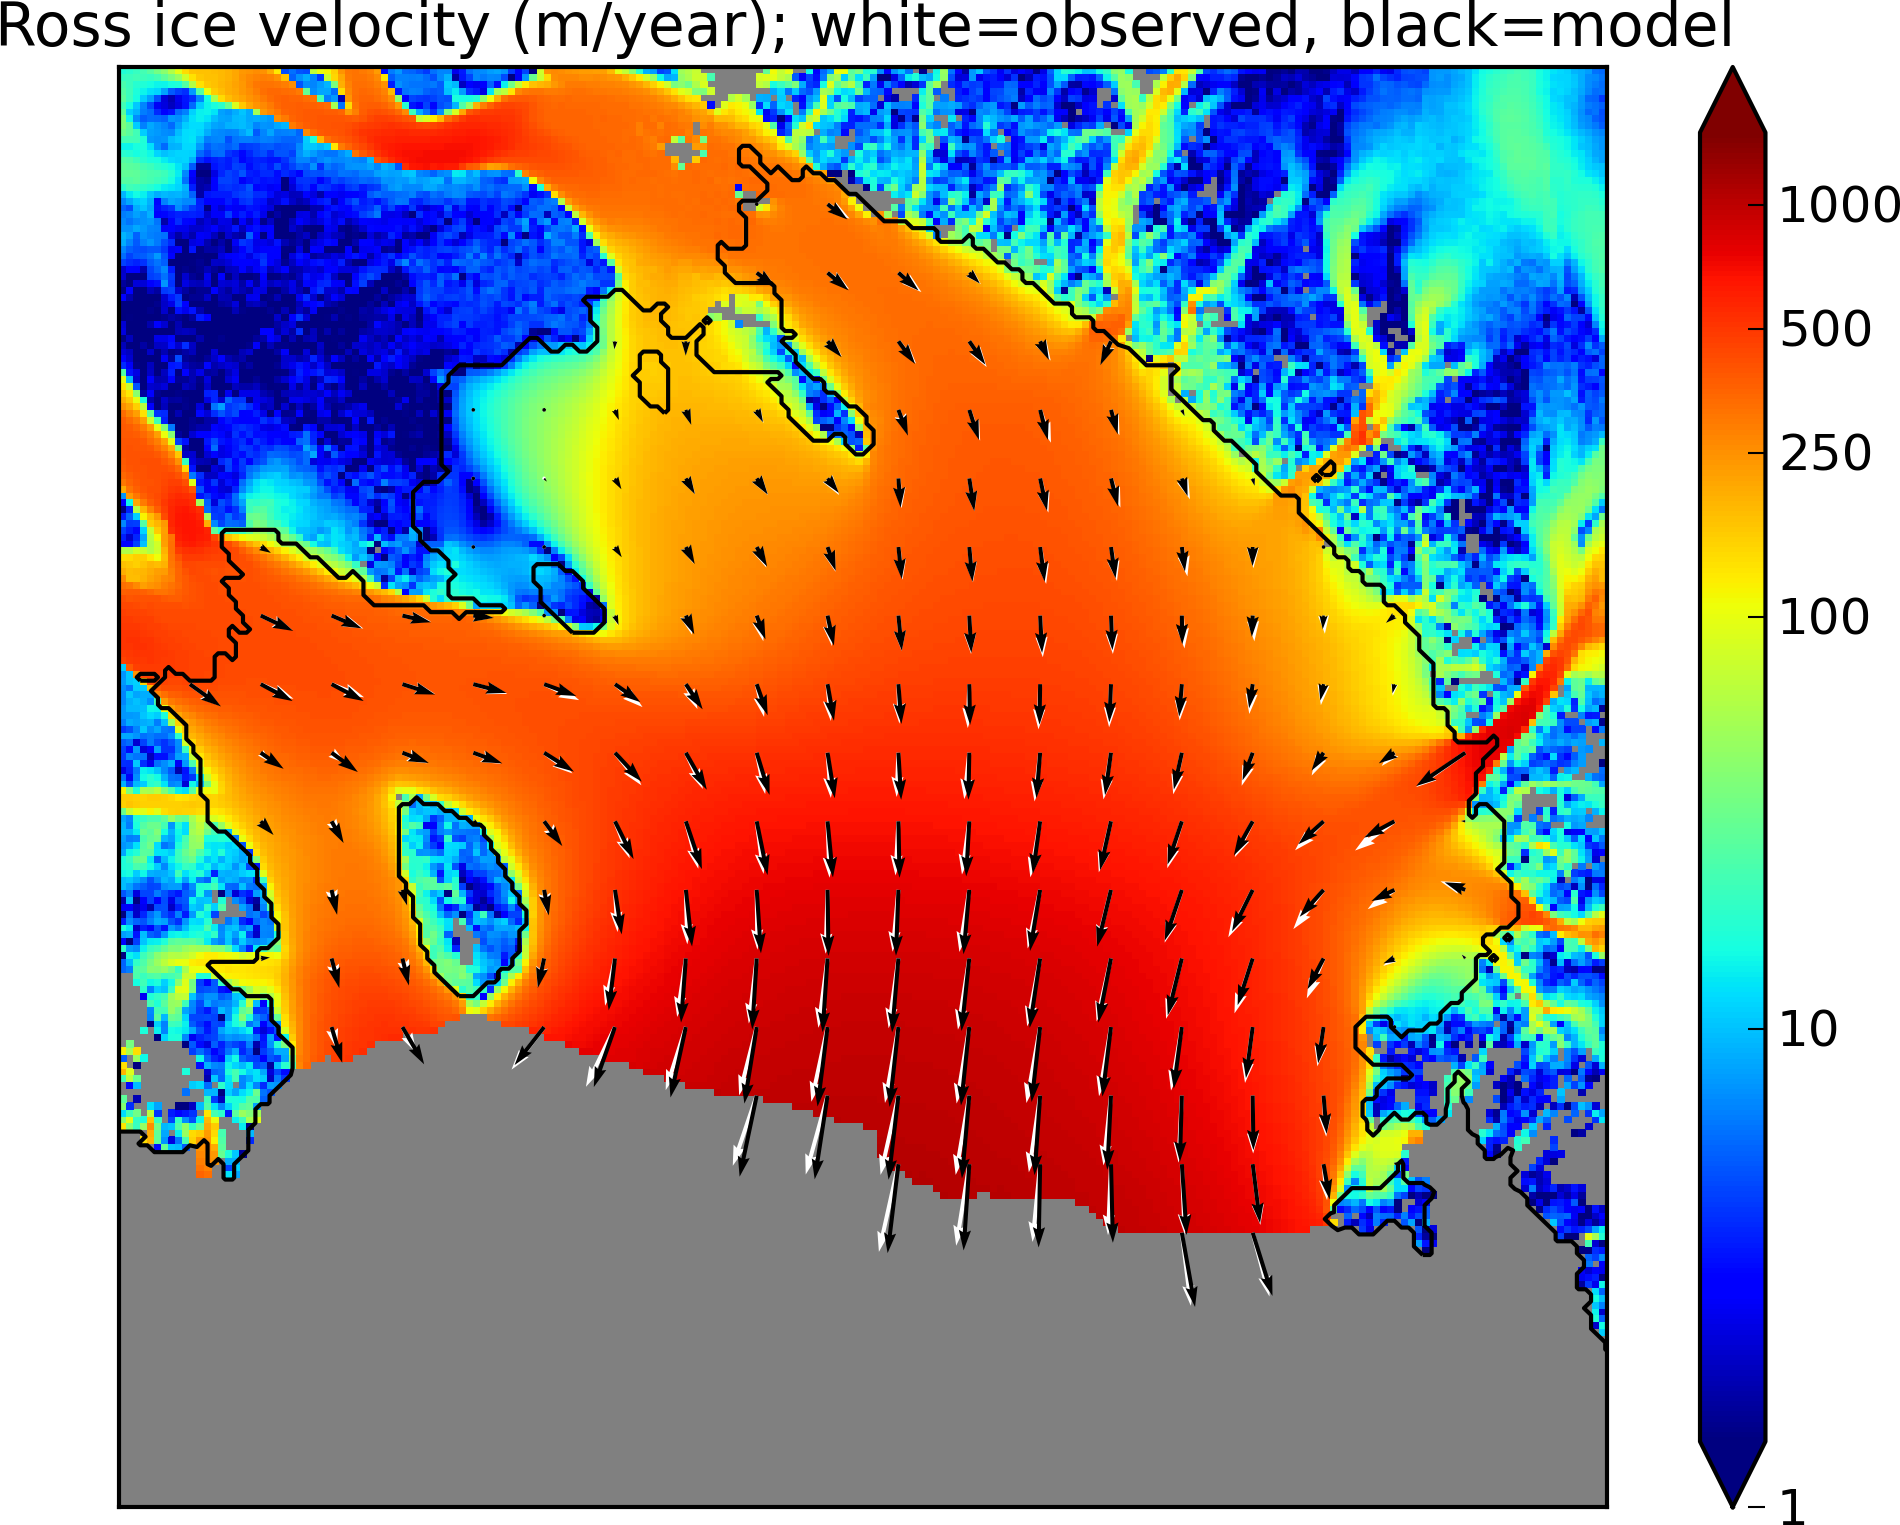
\includegraphics[width=3.3in,keepaspectratio=true]{rossquiver}\quad 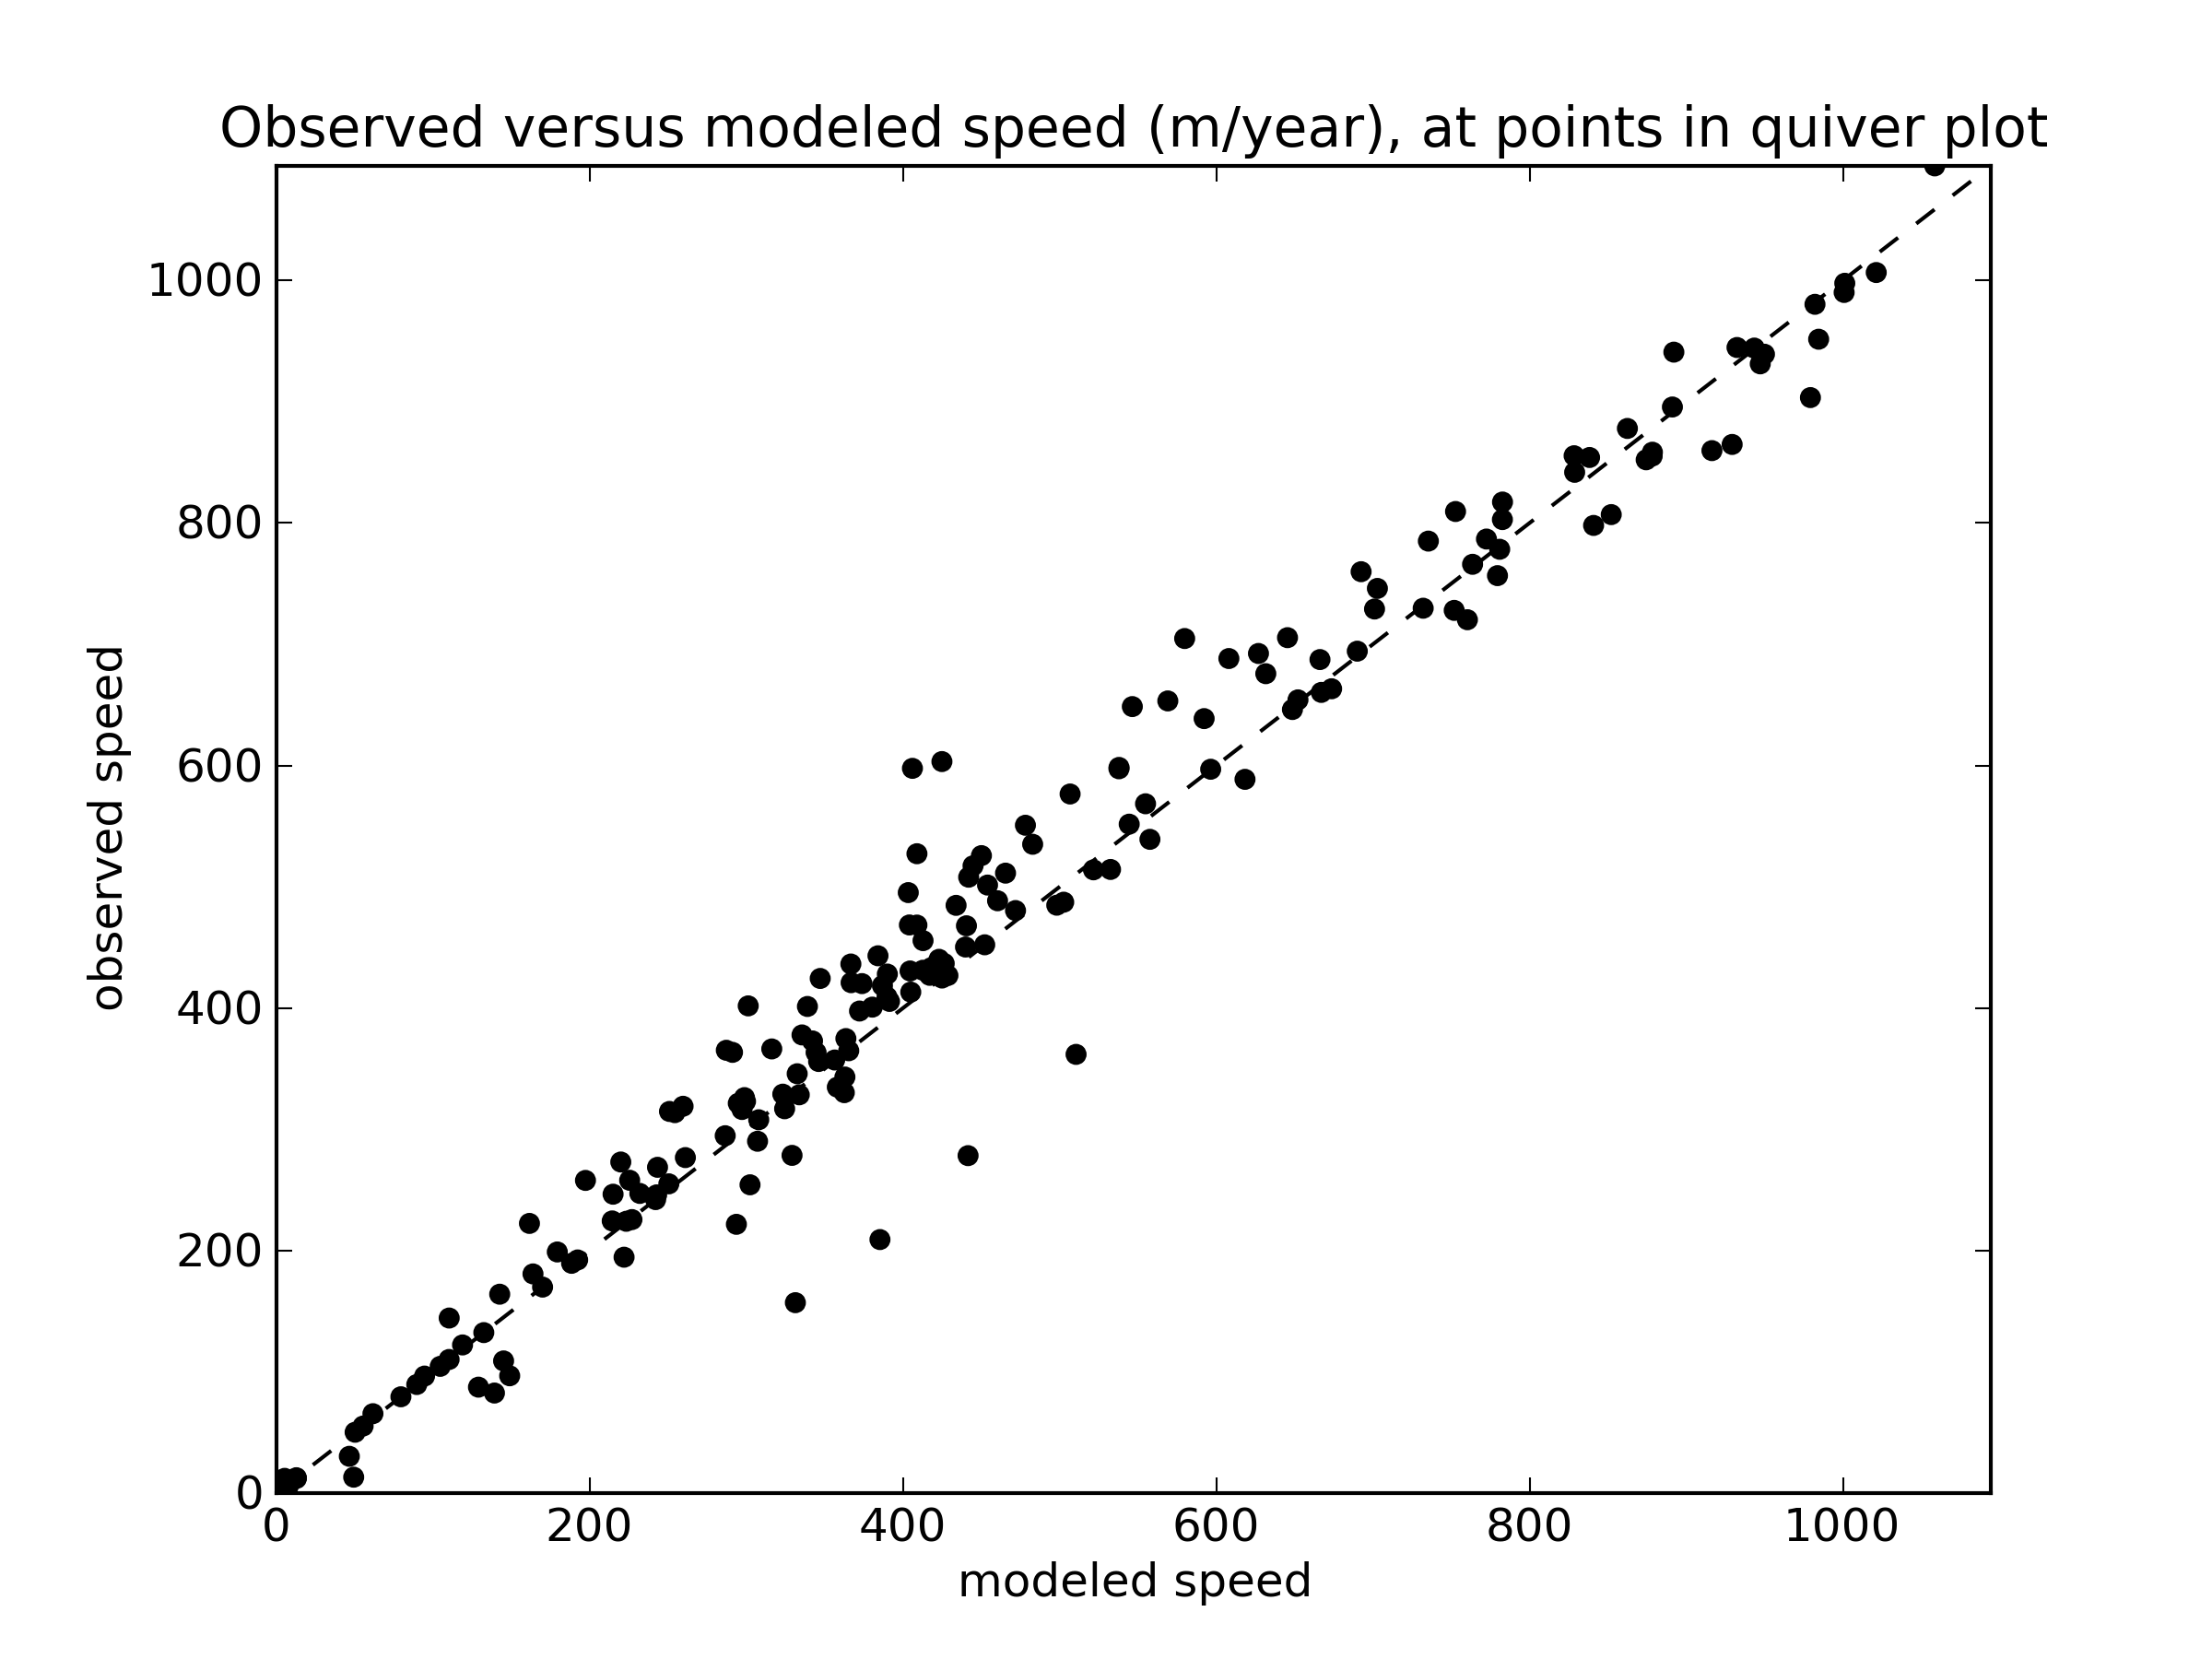
\includegraphics[width=2.7in,keepaspectratio=true]{rossscatter}}
\caption{\protect{\emph{Left}}: Color is speed in m/a.  Arrows are observed (white) and modeled (black) velocities.  \protect{\emph{Right}}: Comparison between modeled and observed speeds at points plotted on the left; compare to Figure \ref{fig:eisrosspython}.}
\label{fig:rosspython}
\end{figure}

\begin{figure}[ht]
\centering
\mbox{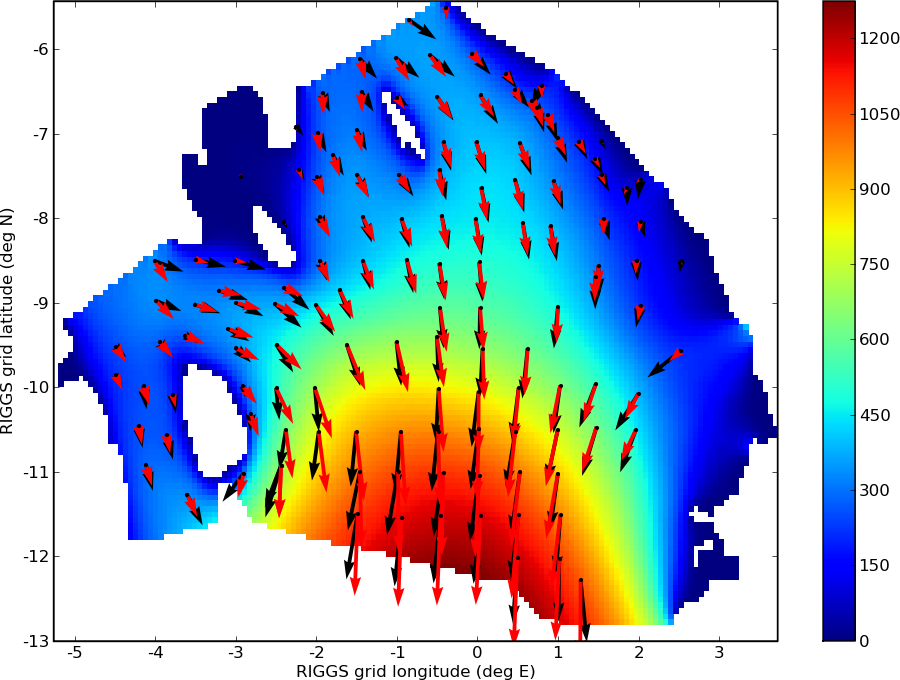
\includegraphics[width=3.3in,keepaspectratio=true]{oldeismintrossquiver}\quad 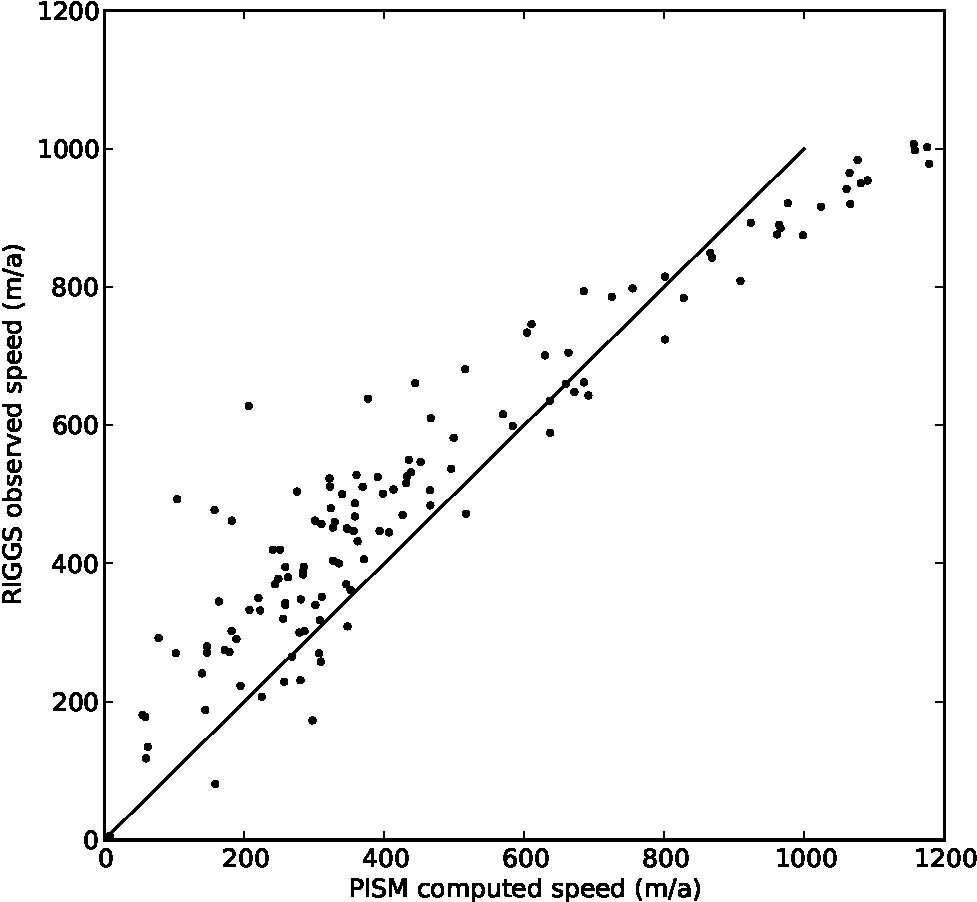
\includegraphics[width=2.7in,keepaspectratio=true]{oldeismintrossscatter}}
\caption{\protect{\emph{Left}}: Color is speed in m/a.  Arrows are observed (black) and computed (red) velocities at RIGGS points.  \protect{\emph{Right}}: Comparison between modeled and observed speeds at RIGGS points; compare Figure 2 in \cite{MacAyealetal}.}
\label{fig:eisrosspython}
\end{figure}

\subsubsection*{Extending this example}

The mechanism described in this section can be easily extended to create flow models of Filchner-Ronne Ice Shelf as in \cite{AlbrechtLevermann2012}, for example. All you need is choose a different part of the domain covered by data-sets used here. See \texttt{preprocess.py} for details.

One can also create a \emph{dynamical} model if an ice shelf with constant-in-time inflow from the grounding line. See scripts in \texttt{examples/ross/prognostic}.

%%% Local Variables:
%%% mode: latex
%%% TeX-master: "manual"
%%% End:


\clearpage\newpage

\section{Example: Storglaci{\"a}ren}\label{sec:storglaciaren} \index{Storglaci{\"a}ren}
\optsection{Storglaci{\"a}ren}

Storglaci{\"a}ren is a small valley glacier in northern Sweden (Figure~\ref{fig:storglaciaren}). The glacier is approximately 3.2\,km long and 1\,km wide, therefore much smaller than a single grid cell in a typical Greenland model. By the way ``Storglaci{\"a}ren'' means ``big glacier'' in Swedish. Most of the glacier is temperate, except for a thin cold near-surface layer in the ablation zone. Such a thermal structure is often-called a Scandinavian-type structure. Thanks to the nearby Tarfala research station it is one of the best investigated glaciers worldwide, and the wealth of data available makes it perfectly suitable for all kinds of modeling studies. In this tutorial we demonstrate how PISM can be used for valley glaciers in a flow-line application. Additionally we show that PISM's conservation of energy scheme is able to simulate the glacier's thermal structure.

\begin{figure}[ht]
  \centering
  \includegraphics[width=3.in,keepaspectratio=true]{storglaciaren}\qquad
  \includegraphics[width=2.75in,keepaspectratio=true]{storglaciaren-dem}
  \caption{Storglaci{\"a}ren, northern Sweden. Left: photo by R. Hock. Right: digital elevation model.}
  \label{fig:storglaciaren}
\end{figure}

To get started run the script \texttt{preprocess.sh} in \texttt{examples/storglaciaren}. It reads the digital elevation model from ASCII files and generates the necessary input files for both the 3-dimensional and the flow-line application. Here we only document the flow-line application.

The mean annual air temperature $T_{\mathrm{MA}}=-6^{\circ}$C at the nearby Tarfala Research Stations serves as the boundary condition for the conservation of energy scheme below the firn line $z_{\textrm{FL}} = 1400$\,m above sea level. Above it, where the ice is temperate, we choose 0$^{\circ}$C. The \texttt{psg_config.cdl} contains parameter choices more suitable for small valley glaciers. Specifically, we increase the limit above which drainge occurs from 1\,\% to 2\,\% liquid water fraction. Furthermore, it sets the till friction angle to 40$^{\circ}$ and the threshold velocity to 10\,m/a.

\texttt{psg_flowline.sh} runs the flow-line application mode. The first two runs smooth the surface and create a more credible enthalpy field. In this example we want to infer the mass balance that has the present day geometry as a steady-state (for now, we ignore the fact that Storglaci{\"a}ren is probably not in a steady-state). As demonstrated in the third run, we can use PISM's mass balance modifier:
\begin{quote}\small
\begin{verbatim}
-surface constant,forcing -force_to_thk psg_flowline_35m_steady.nc -force_to_thk_alpha 0.05
\end{verbatim}
\normalsize\end{quote}
The result of this run is shown in Figure~\ref{fig:storglaciaren-ftt-result}. Without much parameter fine-tuning, simulated surface velocities are reasonably close to observations, c.f. \cite{AschwandenBlatter}.  We also see that a mass balance of about 4 meters per year at the begrschund, almost linearly decreasing to -4.5 meters per year at the tongue, is required to maintain the glaciers geometry. However, observations show that a more realistic present day mass balance decreases lineraly from 2.5 meters per year at the bergschrund to -3 meters per year at the tongue. We now use the surface processes model PSElevation, which is enabled by \texttt{-surface elevation} and allows to define temperature and surface mass balance as a function of surface elevation (see the \emph{PISM's climate forcing components} document for details). The next run uses this present day mass balance which is imposed via 
\begin{quote}\small
\begin{verbatim}
-acab -3,2.5.,1200,1450,1615 -acab_limits -3,0
\end{verbatim}
\normalsize\end{quote} 
For simplicity we assume that the firnline does not change with time. After 25 years the glacier has thinned in the accumulation area but the signal has not yet reached the ablation zone (Figure~\ref{fig:storglaciaren-25a-result}). Plots were produced with the python script \texttt{plot_flowline_results.py}.

\begin{figure}[ht]
  \centering
  \includegraphics[width=5.in,keepaspectratio=true]{sg-flowline-ftt-result}
  \caption{Storglaci{\"a}ren, northern Sweden.  Modeled present day.  Upper panel: horizontal surface velocity (blue solid), basal sliding velocity (blue dashed), and modified surface mass balance (purple) along flowline in meters per year. Lower panel: thermal structure. Red colors indicate liquid water content, blue colors are temperature in degrees Celsius.}
  \label{fig:storglaciaren-ftt-result}
\end{figure}

\begin{figure}[ht]
  \centering
  \includegraphics[width=5.in,keepaspectratio=true]{sg-flowline-25a-result}
  \caption{Storglaci{\"a}ren, northern Sweden. 25\,a model run with present-day surface mass balance. Upper panel: horizontal surface velocity (blue solid), basal sliding velocity (blue dashed), and surface mass balance (purple) along flowline in meters per year. Lower panel: thermal structure. Red colors indicate liquid water content, blue colors are temperature in degrees Celsius.}
  \label{fig:storglaciaren-25a-result}
\end{figure}


%         References
\clearpage\newpage
\bibliography{ice-bib}
\bibliographystyle{siam}

\phantomsection
\addcontentsline{toc}{section}{General Index}
\label{sec:index}
\printindex

\phantomsection
\addcontentsline{toc}{section}{PISM Command-line options}
\printindex[options]


\end{document}
